%# -*- coding:utf-8 -*-
%=========================================================================%
%   LaTeX File for phd thesis of Institute of Automation, CAS
%-------------------------------------------------------------------------%
%
%   revised by Fan Yang (fan.yang@ia.ac.cn) at March, 2013
%
%   * 修正了中英文封面的排版
%   * 修正了参考文献书签定位不准的问题
%   * 修正了书签的层次结构
%   * 为中英文封面和摘要生成书签
%
%-------------------------------------------------------------------------%
%
%   revised by Jian Cheng (jian.cheng.1983@gmail.com) at November, 2011
%
%   * utf8编码,可以工作在texlive in linux 或者 ctex in windows
%   * 生成可以拷贝的中文
%   * 用utf8解决中文书签乱码的问题
%
%-------------------------------------------------------------------------%
%   Revised by Zhaoxiang Zhang (zxzhang@nlpr.ia.ac.cn) at April, 2007
%
%   本模板要求满足GPL协议,可以自行修改并发布,但必须公布代码
%
%-------------------------------------------------------------------------%
%   Revised by J. G. Lou (jglou@nlpr.ia.ac.cn) at April, 2003
%-------------------------------------------------------------------------%
%   Latex 博士论文模板.
%   建议使用miktex2.1最大安装编译此模板
%   本模板使用ctex.org的cjk版本 和aloft 修改后的gb_aloft.cap,
%   如果安装的是miktex包自带的cjk 请用srcbook 替换 book
%=========================================================================%
%%%%%%%%%%%%%%%%%%%%%%%%%%%%%%%%%%%%%%%%%%%%%%%%%%%%%%%%%%%%%%%
%文件头部定义
%%%%%%%%%%%%%%%%%%%%%%%%%%%%%
\documentclass [12pt,a4paper,twoside] {book}
%\documentclass [12pt,a4paper,openany,twoside,draft] {book}
%============================ 引用的宏包 ==================================%
%# -*- coding:utf-8 -*- 
%=========================================================================%
%   LaTeX File for phd thesis of Institute of Automation, CAS
%-------------------------------------------------------------------------%
%   张兆翔将原来的dvipdf改为dvipdfm宏包,可使用latex + dvipdf自动生成索引
%-------------------------------------------------------------------------%
%   Revised by J. G. Lou (jglou@nlpr.ia.ac.cn)
%-------------------------------------------------------------------------%
%=========================================================================%
%                          引用的宏包和相应的定义
%=========================================================================%

%============================ 中文支持宏包 ==============================%
% \usepackage{CJK}
\usepackage{CJKutf8}

%====================== 图形和超链接支持宏包 ========================%
% 图形支持宏包 为了使用PDFLaTeX需要作相应判断
% hyperref
% 可以在转换为pdf文件时自动加入索引, dvi2ps 加入-z 参数
% 为了支持pdftex 使用不同的宏包选项
\ifx\pdfoutput\undefined
\usepackage[dvips]{graphicx}
\usepackage[dvipdfm,
            unicode=true,
            % CJKbookmarks=true,
            bookmarksnumbered=true
            % bookmarksopen=false,
            ]{hyperref}
\else
\usepackage[dvipdfm,
            unicode=true,
            % CJKbookmarks=true,
            bookmarksnumbered=true
            ]{hyperref}
\usepackage[pdftex]{graphicx}
\fi


% \usepackage{ccmap} 


\usepackage{color}      % 支持彩色
\usepackage{subfigure}  % 支持子图
\usepackage{floatflt}   % 图文混排用宏包
\usepackage{rotating}   % 图形和表格的控制
\usepackage{flafter}    % 因为图形可浮动到当前页的顶部,所以它可能会出现
                        % 在它所在文本的前面. 要防止这种情况,可使用 flafter
                        % 宏包

\usepackage[below]{placeins}    %浮动图形控制宏包
                                %允许上一个section的浮动图形出现在下一个
                                %section的开始部分该宏包提供处理浮动对象
                                %的 \FloatBarrier 命令,使所有未处理的浮动
                                %图形立即被处理
%\usepackage{endfloat}  %可将浮动对象放置到文件的最后
%\usepackage{overpic}   %将LaTeX对象放置在图上
%\usepackage{pstricks}  %Postscript macrosfor Generic TeX(我没用过,据说很强)
\usepackage{bez123}

%============================表格支持宏包=================================%
\usepackage{rotating}   % 用法 \begin{sidewaystable}....\end{sidewaystable}
                        % 即可旋转表格
\usepackage{longtable}  % 支持长表格
\usepackage{tabls}
\usepackage{multirow}   % 表格多行合并, 矩阵的边注
\usepackage{colortbl}   % 彩色表格
\usepackage{dcolumn}    % 让表格中将小数点对齐
\usepackage{hhline}     % 在表格中用 \hhline 得到的结果就如同\hline
                        % 或 \hline\hline,当然在和垂直线的交叉处会有所不同。
\usepackage{slashbox}   % 可在表格的单元格中画上一斜线。

%\newcommand{\centpcol}{\leftskip\fill \rightskip\fill}%制表使可用p{ncm}设置栏宽,还使本栏居中

%\iffalse 举例
%  \begin{tabular}{|l|c|c|} \hline
%    & \multicolumn{2}{c|}{MRD} \\ \cline{2-3}
%   & \multicolumn{1}{p{3.5cm}|}{\centpcol Same as previous response} &
%     \multicolumn{1}{p{3.5cm}|}{\centpcol Different from previous response}\\
%   \hline
%    Observed frequency & 966 & 148 \\
%    Expected frequency & 1066 & 48 \\ \hline
%    \multicolumn{3}{c}{${\chi}^2 = 213.97,\quad \mathit{d.f.}=1,\quad p<0.001$}
%  \end{tabular}
%\fi

%============================版面控制宏包=================================%
\usepackage[top=3.0cm,bottom=3.3cm,left=3.2cm,right=3.2cm, headheight=0.5cm, headsep=1.0cm, footskip=1.5cm %,includehead,includefoot
            ]{geometry}                 % 页面设置
\usepackage{indentfirst}                % 首行缩进宏包
\usepackage[perpage,symbol]{footmisc}   % 脚注控制
\usepackage{fancyhdr}                   % fancyhdr宏包 页眉和页脚的相关定义
\usepackage{lastpage}                   %自动记录总页数宏包,计数器为 LastPage
                                        %注意大小写
\usepackage{pageno}     % 章首页的页眉处理, 可以改为自己想要的形式
%\iffalse \makeatletter
%\renewcommand{\ps@plain}{%
%   \renewcommand{\@mkboth}{\@gobbletwo}%
%   \renewcommand{\@evenhead}{\reset@font\sf -- \thepage -- \hfil}%
%   \renewcommand{\@oddhead}{\reset@font\sf\hfil -- \thepage --}%
%   \renewcommand{\@evenfoot}{}%
%   \renewcommand{\@oddfoot}{}
%} \makeatother \fi

%======================= 多列文本与多列编号宏包 ===========================%
\usepackage{multicol,multienum}
%\iffalse 用法为:可嵌套使用
%\begin{multienumerate}[evenlist,oddlist]
%\mitemxxxx{Not}{Linear}{Not}{Quadratic}
%\mitemxxxo{Not}{Linear}{No; if $x=3$, then $y=-2$.}
%\mitemxx{$(x_1,x_2)=(2+\frac{1}{3}t,t)$ or
%$(s,3s-6)$}{$(x_1,x_2,x_3)=(2+\frac{5}{2}s-3t,s,t)$}
%\end{multienumerate}
%\begin{multicols}{2}
%\end{multicols}
%\fi

%======================== 数学公式相关宏包 ===============================%
\usepackage{bm}         % 处理数学公式中的黑斜体的宏包
\usepackage{amsmath}    % AMSLaTeX宏包 用来排出更加漂亮的公式
\usepackage{amssymb}    % AMSLaTeX宏包 用来排出更加漂亮的公式
\usepackage{mathrsfs}  % 不同于\mathcal or \mathfrak 之类的英文花体字体
\usepackage[amsmath,thmmarks]{ntheorem} % 定理类环境宏包,其中 amsmath 选项
                                        % 用来兼容 AMS LaTeX 的宏包
\usepackage{subeqnarray} %多个子方程(1-1a)(1-1b)
%\iffalse 以下是一个例子
%\begin{subeqnarray}
%\label{eqw} \slabel{eq0}
% x & = & a \times b \\
%\slabel{eq1}
% & = & z + t\\
%\slabel{eq2}
% & = & z + t
%\end{subeqnarray}
%\fi

%=============================标题与列表宏包=============================%
\usepackage[sf]{titlesec}   % 控制标题的宏包,配合命令在后面,
                            % 将cjk+miktex+scrbook+gb.cap下的章的标题号,
                            % 比如~``第二章 XXX''位置于中心
\usepackage{cite}           % 支持引用的宏包
\usepackage{enumerate}      % 改变列表标号样式宏包 其后可接选项[a,A,i,I,1]
\usepackage{caption2}       % 浮动图形和表格标题样式,可选项为
                            % [scriptsize,footnotesize,centerlast]
%\usepackage{setspace}      % 图形和表格的标题如果是多行,行距比较大,可以加宏包
\usepackage{pifont}         % 有很漂亮的带圈的各种数字符号使用
%\usepackage{atbeginend}    % 可选宏包, 能解决许多问题,
                            % 比如itemize, enumerate环境\item之间的控制
%用法
%\AfterBegin{itemize}{\addtolength{\itemsep}{-0.5\baselineskip}}
%\AfterBegin{enumerate}{\addtolength{\itemsep}{-0.5\baselineskip}}

%=================== 支持LaTexCAD生成的源程序的宏包 =====================%
\usepackage{TEXcad/lgrind}     % for formated source code
\usepackage{TEXcad/latexcad}   % latexcad.sty for drawings etc
\usepackage{TEXcad/epic}       %picture macros
\usepackage{TEXcad/eepic}      %extended picture macros
\usepackage{TEXcad/fancybox}   %box macros
\usepackage{TEXcad/epsf}       %postscript macros
\usepackage{TEXcad/rotate}     % postscript text rotation macros


%=========================== 特殊文本元素宏包 ==============================%
\usepackage{nicefrac}   % 在正文文本中排版分式时,可以用它来得到较好的排版效果。
\usepackage{units}      % 基于 nicefrac 宏包,提供对计量单位比较美观的排版效果。
\usepackage{soul}       % 支持对单词加上下划线或其每个字母在一定的宽度内均匀散布
\usepackage{altfont}    % 使用该宏包, 可以在一个宏包中使用多种不同的字体,
                        % 包括PSNFSS 和 MFNFSS
%\usepackage{prelim2e}  % 可以在每页页脚下方标记出本文档的版本信息等
\usepackage{a0size}     % 自由定义字号,在后面“字号设置”中可设置到107pt为止的大字体
%\usepackage{ulem}      % 用于支持文字内容的删除(非latex源文件中的注释!)(对中文的支持不够好,不会换行)
\usepackage{CJKulem}    % 用于支持文字内容的删除(非latex源文件中的注释!)(CJK字体专用)

\begin{document}
\begin{CJK*}{UTF8}{song}



\graphicspath{{figures/}}   %定义所有的eps文件在 image 子目录下

%=========================== 文本格式定义 =================================%
%# -*- coding:utf-8 -*-
%=========================================================================%
%   LaTeX File for phd thesis of Institute of Automation, CAS
%-------------------------------------------------------------------------%

%=========================================================================%
%                          主文档 格式定义
%=========================================================================%

%===================== 重定义字体、字号命令 =============================%
% 注意win2000,没有 simsun, 最好到网上找一个。一些字体是office2000带的
\newcommand{\song}{\CJKfamily{song}}    % 宋体   (Windows自带simsun.ttf)
\newcommand{\fs}{\CJKfamily{fs}}        % 仿宋体 (Windows自带simfs.ttf)
\newcommand{\kai}{\CJKfamily{kai}}      % 楷体   (Windows自带simkai.ttf)
\newcommand{\hei}{\CJKfamily{hei}}      % 黑体   (Windows自带simhei.ttf)
\newcommand{\li}{\CJKfamily{li}}        % 隶书   (Windows自带simli.ttf)
\newcommand{\you}{\CJKfamily{you}}      % 幼圆   (Windows自带simyou.ttf)
\newcommand{\chuhao}{\fontsize{42pt}{\baselineskip}\selectfont}     % 字号设置
\newcommand{\xiaochuhao}{\fontsize{36pt}{\baselineskip}\selectfont} % 字号设置
\newcommand{\yihao}{\fontsize{28pt}{\baselineskip}\selectfont}      % 字号设置
\newcommand{\erhao}{\fontsize{21pt}{\baselineskip}\selectfont}      % 字号设置
\newcommand{\xiaoerhao}{\fontsize{18pt}{\baselineskip}\selectfont}  % 字号设置
\newcommand{\sanhao}{\fontsize{15.75pt}{\baselineskip}\selectfont}  % 字号设置
\newcommand{\sihao}{\fontsize{14pt}{\baselineskip}\selectfont}      % 字号设置
\newcommand{\xiaosihao}{\fontsize{12pt}{\baselineskip}\selectfont}  % 字号设置
\newcommand{\wuhao}{\fontsize{10.5pt}{\baselineskip}\selectfont}    % 字号设置
\newcommand{\xiaowuhao}{\fontsize{9pt}{\baselineskip}\selectfont}   % 字号设置
\newcommand{\liuhao}{\fontsize{7.875pt}{\baselineskip}\selectfont}  % 字号设置
\newcommand{\qihao}{\fontsize{5.25pt}{\baselineskip}\selectfont}    % 字号设置

%===================================================================%
%                         各种距离与缩进
%===================================================================%

%-------------------- 用于中文段落缩进 和正文版式 ------------------%
\CJKcaption{Setup/GB_aloft_UTF8}
\setlength{\parindent}{2em}                 % 首行两个汉字的缩进量
\setlength{\parskip}{3pt plus1pt minus1pt}  % 段落之间的竖直距离
\renewcommand{\baselinestretch}{1}        % 定义行距

%------------------------- 列表与图表距离设置 -----------------------%
\setlength{\topsep}{2pt plus1pt minus2pt}           % 第一个item和前面版落间的距离
\setlength{\partopsep}{3pt plus1pt minus2pt}        % 当在一个新页开始时加到
                                                    % \topsep的额外空间
\setlength{\itemsep}{3pt plus1pt minus2pt}          % 连续items之间的距离.
\setlength{\floatsep}{10pt plus 3pt minus 2pt}      % 图形之间或图形与正文之间的距离
\setlength{\abovecaptionskip}{2pt plus1pt minus1pt} % 图形中的图与标题之间的距离
\setlength{\belowcaptionskip}{3pt plus1pt minus2pt} % 表格中的表与标题之间的距离

%下面这组命令使浮动对象的缺省值稍微宽松一点,从而防止幅度
%对象占据过多的文本页面,也可以防止在很大空白的浮动页上放置
%很小的图形。
\renewcommand{\textfraction}{0.15}
\renewcommand{\topfraction}{0.85}
\renewcommand{\bottomfraction}{0.65}
\renewcommand{\floatpagefraction}{0.60}

%---------------------------- 数学公式设置 ------------------------------%
\setlength{\abovedisplayskip}{2pt plus1pt minus1pt}     %公式前的距离
\setlength{\belowdisplayskip}{2pt plus1pt minus1pt}     %公式后面的距离
\setlength{\arraycolsep}{2pt}   %在一个array中列之间的空白长度, 因为原来的太宽了

\allowdisplaybreaks[4]  % \eqnarray如果很长,影响分栏、换行和分页
                        %(整块挪动,造成页面空白),可以设置成为自动调整模式

%===================================================================%
%                         各种标题样式
%===================================================================%
%======================= 标题名称中文化 ============================%
\renewcommand\contentsname{目\ 录}
\renewcommand\listfigurename{插图目录}
\renewcommand\listtablename{表格目录}
%\renewcommand\abstractname{摘\ 要} %err undefined
%\renewcommand\refname{参考文献}         %article类型
\renewcommand\bibname{参\ 考\ 文\ 献}    %book类型
\renewcommand\indexname{索\ 引}
\renewcommand\figurename{图}
\renewcommand\tablename{表}
\renewcommand\partname{部分}


%======================= 定制章节的标题样式 =============================%
\setcounter{secnumdepth}{3}
%---------------------- 定义章节的编号格式 --------------------------%
%\renewcommand{\thesection}{\CJKnumber{\arabic{section}}、} % 定义 一、。九、十
\renewcommand{\thesection}{\arabic{chapter}.\arabic{section}}
\renewcommand{\thesubsection}{\arabic{chapter}.\arabic{section}.\arabic{subsection}}
\renewcommand{\thesubsubsection}{\arabic{chapter}.\arabic{section}.\arabic{subsection}.\arabic{subsubsection}}
\let\oldtitle=\title
\def\title#1{\oldtitle{\cnbf{#1}}}
\renewcommand{\CJKglue}{\hskip 0pt plus 0.08\baselineskip}

%----------------------- 定义章节标题格式 ----------------------------%
\titleformat{\chapter}[hang]{\fontsize{15pt}{15pt}\selectfont\filcenter\CJKfamily{hei}}
    {\fontsize{15pt}{15pt}\selectfont{\chaptertitlename}}{20pt}{\fontsize{15pt}{15pt}\selectfont}
\titlespacing{\chapter}{0pt}{-3ex  plus .1ex minus .2ex}{2.5ex plus .1ex minus .2ex}

%\titleformat{\section}[hang]{\CJKfamily{hei}\Large \centering} %标题居中
\titleformat{\section}[hang]{\CJKfamily{hei}\fontsize{14pt}{14pt}\selectfont}
    {\fontsize{14pt}{17pt}\selectfont \thesection}{1em}{}{}
\titlespacing{\section}
    {0pt}{1.5ex plus .1ex minus .2ex}{\wordsep}

\titleformat{\subsection}[hang]{\CJKfamily{hei}\fontsize{13pt}{13pt}\selectfont}
    { \fontsize{13pt}{13pt}\selectfont\thesubsection}{1em}{}{}
\titlespacing{\subsection}%
    {0pt}{1.5ex plus .1ex minus .2ex}{\wordsep}

\titleformat{\subsubsection}[hang]{\CJKfamily{hei}\fontsize{12pt}{12pt}\selectfont}
    {\fontsize{12pt}{12pt}\selectfont\thesubsubsection}{1em}{}{}
\titlespacing{\subsubsection}%
    {0pt}{1.2ex plus .1ex minus .2ex}{\wordsep}

%======================= 定义列表项目格式 ==========================%
\renewcommand\labelenumi{\textcircled{\scriptsize \theenumi}}  %带圈的数字
%\renewcommand\labelenumi{(\theenumi)}
\renewcommand\labelenumii{(\theenumii)}
\renewcommand\labelenumiii{\theenumiii.}
\renewcommand\labelenumiv{\theenumiv.}

%====================== 定制图形和表格标题样式 =====================%
%---------------------- 定制图形和表格标题格式 ---------------------%
%\renewcommand{\captionlabeldelim}{}
\captionsetup{labelsep=space}
\renewcommand{\captionlabelfont}{\small \CJKfamily{hei}\bf}
\renewcommand{\captionfont}{\small \CJKfamily{song}\rmfamily}
%% \scriptsize \footnotesize \small \large \Large  %图形标签字体大小

%--------------------- 定义图、表、公式的编号格式 -------------------%
\renewcommand{\thetable}{\arabic{chapter}-\arabic{table}}
\renewcommand{\theequation}{\arabic{chapter}-\arabic{equation}}
\renewcommand{\thefigure}{\arabic{chapter}-\arabic{figure}}


%=========================== 目录设置 ==================================%
\setcounter{tocdepth}{3} \setcounter{secnumdepth}{3}
% 可以用\section[abc]{abcdefg}形式的命令,这样abc就做为缩短标题出现
% 在目录表中和页眉上.另外,还可以利用\addtocounter{secnumdepth}{num}
% 来使得当前章节编号深度增加或减小,num可取正值或负值.

%============================= 页面设置 ================================%
%-------------------- 定义页眉和页脚 使用fancyhdr 宏包 -----------------%
\newcommand{\makeheadrule}{%
    %\makebox[0pt][l]{\rule[.7\baselineskip]{\textwidth}{1.2pt}}
    \rule[.6\baselineskip]{\linewidth}{0.4pt}\vskip-.8\baselineskip}
\makeatletter
\renewcommand{\headrule}{%
    {\if@fancyplain\let\headrulewidth\plainheadrulewidth\fi
     \makeheadrule }} %
\makeatother                                % 定义页眉与正文间隔线

\pagestyle{fancyplain}
\renewcommand{\chaptermark}[1]%
{\markboth{\chaptername \ #1}{}}            % 去掉章节标题中的数字
\fancyhf{} %\fancyfoot[C,C]{\thepage}

\fancyhead[CO]{\CJKfamily{fs}\leftmark}          % 在book文件类别下,
\fancyhead[CE]{\CJKfamily{fs}\rightmark}         % \leftmark自动存录各章之章名,

\fancyfoot[C]%                                  % [RE][LO]
{\CJKfamily{hei} -\;\thepage\;-}

%=== 配合前面的ntheorem宏包产生各种定理结构,重定义一些正文相关标题 ===%
\theoremstyle{plain}
\theoremheaderfont{\normalfont\rmfamily\CJKfamily{hei}}
\theorembodyfont{\normalfont\rm\CJKfamily{kai}} \theoremindent0em
%\theorembodyfont{\normalfont\rm\CJKfamily{song}} \theoremindent0em
\theoremseparator{:} \theoremnumbering{arabic}
%\theoremseparator{\hspace{1em}} \theoremnumbering{arabic}
%\theoremsymbol{}          %定理结束时自动添加的标志
%\newtheorem{definition}{\noindent定义}[chapter]
\newtheorem{definition}{\hspace{2em}定义}[chapter]
%\newtheorem{definition}{\hei 定义}[section] %!!!注意当section为中国数字时,[sction]不可用!
\newtheorem{proposition}{\hspace{2em}命题}[chapter]
\newtheorem{property}{\hspace{2em}性质}[chapter]
\newtheorem{lemma}{\hspace{2em}引理}[chapter]
%\newtheorem{lemma}[definition]{引理}
\newtheorem{theorem}{\hspace{2em}定理}[chapter]
\newtheorem{axiom}{\hspace{2em}公理}[chapter]
\newtheorem{corollary}{\hspace{2em}推论}[chapter]
\newtheorem{exercise}{\hspace{2em}习题}[chapter]
%\theoremsymbol{$\blacksquare$}
\newtheorem{example}{\hspace{2em}例}[chapter]

\theoremstyle{nonumberplain}
\theoremheaderfont{\CJKfamily{hei}\rmfamily}
\theorembodyfont{\normalfont \rm \CJKfamily{song}}
\theoremindent0em \theoremseparator{\hspace{1em}}
\theoremsymbol{$\blacksquare$}
\newtheorem{proof}{\hspace{2em}证明:}

%=========================== 修改引用的格式 ==============================%
% 第一行在引用处数字两边加方框
% 第二行去除参考文献里数字两边的方框
%\makeatletter
%\def\@cite#1{\mbox{$\m@th^{\hbox{\@ove@rcfont[#1]}}$}}
%\renewcommand\@biblabel[1]{#1}
%\makeatother
% 增加 \upcite 命令使显示的引用为上标形式
%\newcommand{\upcite}[1]{$^{\mbox{\scriptsize \cite{#1}}}$}             % 方法1
\newcommand{\upcite}[1]{\textsuperscript{\textsuperscript{\cite{#1}}}}  % 方法2


%=============================== 脚注 =============================%
\renewcommand{\thefootnote}{\arabic{footnote}}
%detcounter{footnote}{0}

%==================== 定义题头格言的格式 ==========================%
% 用法 \begin{Aphorism}{author}
%         aphorism
%      \end{Aphorism}
\newsavebox{\AphorismAuthor}
\newenvironment{Aphorism}[1]
{\vspace{0.5cm}\begin{sloppypar} \slshape
\sbox{\AphorismAuthor}{#1}
\begin{quote}\small\itshape }
{\\ \hspace*{\fill}------\hspace{0.2cm} \usebox{\AphorismAuthor}
\end{quote}
\end{sloppypar}\vspace{0.5cm}}

%============================== 控制表格线宽 ==========================%
% 更改横线(\hline)线宽:定义如下命令\hlinewd代替\hline。
% 更改垂直线(\vline)线宽:使用\usapackage{array},则可以在指定垂直线的地方用
% “!{\vrule width 3.5pt}”代替“|”,如“|c!{\vrule width 5pt}p{5cm}|r|”

\makeatletter
\def\hlinewd#1{%
  \noalign{\ifnum0=`}\fi\hrule \@height #1 \futurelet
   \reserved@a\@xhline}
\makeatother
\newcommand\vlinewd[1][1pt]{\vrule width #1}

% 不过上面的命令\hlinewd不能与longtable正常工作(reported by %钟圣俊老师),
% 只能使用下面的方法实现线宽控制:
%
%\setlength{\arrayrulewidth}{0.5pt}
%\setlength{\doublerulesep}{\arrayrulewidth}
%\newcommand{\dhline}{\hline\hline}
%\newcommand{\thline}{\hline\hline\hline}
%(类似的可以定义更多不同宽度的\hline)


%========================== 其它自定义 ==============================%
%====================================================================%
% 下面定义的命令(\alpheqn \reseteqn)可以使公式编号变为 4-a,4-b
% 使用说明:\alpheqn 为开始产生处,\reseteqn为恢复原来公式编号形式处
% 这两个命令为自定义,使用时应注意:不可放于 数学环境中!!!
% 在公式开始前和结束后使用!!!
%====================================================================%
\newcounter{saveeqn}%

\newcommand{\alpheqn}{%
\setcounter{saveeqn}{\value{equation}}%
\stepcounter{saveeqn}%
\setcounter{equation}{0}%
%\renewcommand{\theequation}{\arabic{saveeqn}-\alph{equation}}}%%article 中的定义
\renewcommand{\theequation}{\arabic{chapter}-\arabic{saveeqn}\alph{equation}}}%book %中的定义
%{\mbox{\arabic{equation}-\alph{equation}}}}%

\newcommand{\reseteqn}{%
\setcounter{equation}{\value{saveeqn}}%
%%\renewcommand{\theequation}{\arabic{equation}}}    %article 中的定义
\renewcommand{\theequation}{\arabic{chapter}-\arabic{equation}}}  %book 中的定义

%====================================================================%
% 下面定义的命令(\alphfig \resetfig)可以使插图编号变为 4-a,4-b
% 使用说明:\alphfig 为开始产生处,\resetfig为恢复原来插图编号形式处
% 这两个命令为自定义,使用时应注意:不可放于 数学环境中!!!
% 在插图开始前和结束后使用!!!
%====================================================================%
\newcounter{savefig}%

\newcommand{\alphfig}{%
\setcounter{savefig}{\value{figure}}%
\stepcounter{savefig}%
\setcounter{figure}{0}%
%%\renewcommand{\thefigure}{\arabic{savefig}-\alph{figure}}}%%article 中的定义
\renewcommand{\thefigure}{\arabic{chapter}-\arabic{savefig}\alph{figure}}}%book 中的定义
%{\mbox{\arabic{figure}-\alph{figure}}}}%

\newcommand{\resetfig}{%
\setcounter{figure}{\value{savefig}}%
%%\renewcommand{\thefigure}{\arabic{figure}}}    %article 中的定义
\renewcommand{\thefigure}{\arabic{chapter}-\arabic{figure}}}  %book 中的定义

%====================================================================%
% 下面定义的命令(\alphtab \resettab)可以使表格编号变为 4-a,4-b
% 使用说明:\alphtab 为开始产生处,\resettab为恢复原来表格编号形式处
% 这两个命令为自定义,使用时应注意:不可放于 数学环境中!!!
% 在表格开始前和结束后使用!!!
%====================================================================%
\newcounter{savetab}%

\newcommand{\alphtab}{%
\setcounter{savetab}{\value{table}}%
\stepcounter{savetab}%
\setcounter{table}{0}%
%%\renewcommand{\thetable}{\arabic{savetab}-\alph{table}}}%%article 中的定义
\renewcommand{\thetable}{\arabic{chapter}-\arabic{savetab}\alph{table}}}%%book 中的定义
%{\mbox{\arabic{table}-\alph{table}}}}%

\newcommand{\resettab}{%
\setcounter{table}{\value{savetab}}%
%%\renewcommand{\thetable}{\arabic{table}}}    %article 中的定义
\renewcommand{\thetable}{\arabic{chapter}-\arabic{table}}}  %book 中的定义

%====================================================================%
% 自定义项目列表标签及格式 \begin{mylist} 列表项 \end{mylist}
%====================================================================%
\newcounter{newlist} %自定义新计数器
\newenvironment{mylist}[1][可改变的列表题目]{%%%%%定义新环境
\begin{list}{\textbf{\hei #1} \arabic{newlist}:} %%标签格式
    {
    \usecounter{newlist}
     \setlength{\labelwidth}{22pt} %标签盒子宽度
     \setlength{\labelsep}{0cm} %标签与列表文本距离
     \setlength{\leftmargin}{0cm} %左右边界
     \setlength{\rightmargin}{0cm}
     \setlength{\parsep}{0.5ex plus0.2ex minus0.1ex} %段落间距
     \setlength{\itemsep}{0ex plus0.2ex} %标签间距
     \setlength{\itemindent}{44pt} %标签缩进量
     \setlength{\listparindent}{22pt} %段落缩进量
    }}
{\end{list}}%%%%%


%============================== 封面 ======================================%
\renewcommand{\baselinestretch}{1.6}    %\baselineskip 的倍数,两者相乘为行间距。
\fontsize{14.75pt}{12pt}\selectfont     %\fontsize{size}{skip}skip相当于\baselineskip
%\cleardoublepage
%\phantomsection
%\addcontentsline{toc}{part}{经皮介入冠脉导管术仿真系统中创建解剖环境的关键技术研究}
%\addcontentsline{toc}{chapter}{封面}
%# -*- coding:utf-8 -*- 
%=========================================================================%
%   LaTeX File for phd thesis of Institute of Automation, CAS
%-------------------------------------------------------------------------%
%   Revised by J. G. Lou (jglou@nlpr.ia.ac.cn)
%   封面
%-------------------------------------------------------------------------%

\thispagestyle{empty} %取消当前页码

\vspace*{0.5cm} %插入空白
\begin{tabbing}
%样本行
\hspace*{-0.8cm} \= \hspace{9.4cm} \= \kill

\>{\wuhao 分类号} \underline{\hspace{2.8cm}} \>{\wuhao 密级}\underline{\hspace{3.3cm}}\\

\>{\wuhao UDC} \underline{\hspace{3.1cm}} \> {\wuhao 编号}\underline{\hspace{3.3cm}}\\
\end{tabbing}

\vspace*{1.7cm} %插入空白
\begin{center}
{\Huge \song \textbf{中国科学院大学}}\\
\vspace{0.8cm} {\Huge \song \textbf{博士学位论文}}\\
\vspace{1.8cm}
{\xiaoerhao \song \underline{经皮介入冠脉导管术仿真系统的关键技术研究}}\\
\vspace{1.1cm} {\sanhao \underline{\;杨\;\;\;\;帆\;}}\\
\end{center}
\sanhao \vspace{1.2cm}
\begin{tabbing}
%样本行
\hspace*{-0.8cm} \= \hspace{6.4cm} \= \kill

\>指导教师\underline{\hspace{4.8cm}侯增广\;\;研究员\hspace{4.6cm}}\\

\>\hspace{2.0cm} \underline{\hspace{13.1cm}}\\

\>申请学位级别\underline{\hspace{0.5cm}工学博士\hspace{0.5cm}} \>学科专业名称 \underline{\hspace{0.2cm}控制理论与控制工程\hspace{0.2cm}}\\

\>论文提交日期\underline{\hspace{0.3cm}2013年11月\hspace{0.3cm}} \> 论文答辩日期\underline{\hspace{1.4cm}2013年12月\hspace{1.4cm}}\\

\>培养单位 \underline{\hspace{3.5cm}中国科学院自动化研究所 \hspace{3.5cm}} \\

\>学位授予单位\underline{\hspace{3.5cm}中国科学院大学 \hspace{4.6cm}} \\
\end{tabbing}
\vspace{0.5cm}
\hspace*{7.1cm}答辩委员会主席\underline{\hspace{3.4cm}}
 %中文封面
%插入空白页
\include{cover/blank_UTF8}
\cleardoublepage
\phantomsection
%\addcontentsline{toc}{chapter}{Cover}
%# -*- coding:utf-8 -*-
%=========================================================================%
%   LaTeX File for phd thesis of Institute of Automation, CAS
%-------------------------------------------------------------------------%
%   Revised by J. G. Lou (jglou@nlpr.ia.ac.cn)
%   封面
%-------------------------------------------------------------------------%

{\renewcommand{\baselinestretch}{1.0}

\thispagestyle{empty} %取消当前页码

\vspace*{0.5cm} %插入空白
\begin{center}
  {\xiaoerhao \hei \textsf{\textbf{\underline{Research on Key Technologies}\\
  \underline{for Visualization of Anatomical Environment}\\
  \underline{in Coronary Intervention Simulation}
  }}}
\end{center}

\vspace*{3.5cm} %插入空白
\begin{center}

\textsf{\sanhao \textrm{\textbf{By}}}\\
\textsf{\sanhao \textrm{\textbf{Fan Yang}}}

\vspace*{2.0cm} %插入空白
\xiaosihao \textrm{\textbf{ A Dissertation Submitted to\\
University of Chinese Academy of Sciences\\
In partial fulfillment of the requirements\\
For the degree of\\
Doctor of Engineering\\
In Control Theory and Control Engineering}}
\end{center}

\begin{center}
\vspace{1.5cm}
\xiaosihao \textrm{\textbf{Institute of Automation, Chinese Academy of Sciences}}\\
\wuhao \textrm{\textbf{December, 2014}}
\end{center}
}  %英文封面
%插入空白页
\include{cover/blank_UTF8}
%\cleardoublepage
%\phantomsection
%\addcontentsline{toc}{chapter}{独创性声明}
%# -*- coding:utf-8 -*- 
\thispagestyle{empty} %取消当前页码
\vspace*{1.0cm}

\centerline{\erhao \song \textsf{\textbf{独创性声明}}}
\vspace*{0.5cm}
{\small
本人声明所递交的论文是我个人在导师指导下进行的研究工作及取得的研究成果。
尽我所知,除了文中特别加以标注和致谢的地方外,论文中不包含其他人已经发
表或撰写过的研究成果。与我一同工作的同事对本研究所做的任何贡献均已在论
文中作了明确地说明并表示了谢意。

\hspace*{4.5cm}签~名:\underline{\hspace{3.0cm}}日~期:\underline{\hspace{3.0cm}}}

\vspace*{3.0cm}

\centerline{\erhao \song \textsf{\textbf{关于论文使用授权的说明}}}
\vspace*{0.5cm}
{\small
本人完全了解中国科学院自动化研究所有关保留、使用学位论文的规定,即:中国
科学院自动化研究所有权保留送交论文的复印件,允许论文被查阅和借阅;可以公
布论文的全部或部分内容,可以采用影印、缩印或其他复制手段保存论文。\\
{\bf(保密的论文在解密后应遵守此规定)}
\vspace*{3.5cm}

\centerline{签~名:\underline{\hspace{3.0cm}}导师签名:\underline{\hspace{3.0cm}}日~期:\underline{\hspace{3.0cm}}}
}
 %独创性声明
\renewcommand{\baselinestretch}{1.6}
\include{cover/blank_UTF8}
%============================= 导言部分 ===================================%
\frontmatter        %导言部分页码自动为罗马数字
\sloppy             %放松拆行的限制解决中英文混排的断行问题,会加入间距,但
                    %不会影响断行
\fontseries{mex}
%中文摘要
\renewcommand{\baselinestretch}{1.2}
\fontsize{12pt}{12pt}\selectfont
\cleardoublepage
\phantomsection
\addcontentsline{toc}{chapter}{摘要}
%# -*- coding:utf-8 -*-
%=========================================================================%
%   LaTeX File for phd thesis of Institute of Automation, CAS
%-------------------------------------------------------------------------%
%   Revised by J. G. Lou (jglou@nlpr.ia.ac.cn)
%   中文摘要页
%-------------------------------------------------------------------------%
\chapter*{摘\;\;\;要 \markboth{摘\;\;要}{摘\;\;要}}

\vspace{0.5cm} \wuhao
%以下为摘要的正文

在本文中,我们研究了经皮冠状动脉介入术仿真训练系统的关键技术。研究工作的重点集
中在与经皮冠状动脉介入术这一被大量采用的治疗冠心病的治疗技术过程相关的人体解剖
环境模型的生成方面,尤其关注基于CTA体数据的血管系统模型的建立和心脏模型的建立。
在传统的手术操作和学习过程、尤其是学习过程中,仍存在着一些不足,例如:见习机会
的稀缺,活体动物的高成本,以及培训考核中评估意见的主观性等。仿真训练系统为解决
这些问题提供了可能性。本文的贡献在于对这种仿真训练系统的关键技术的研究。

本文的关注点在于与经皮冠状动脉介入术相关的血管系统等人体解剖结构的几何建模和物
理建模。在这一能够表达出恰当物理特性的解剖环境模型中,虚拟手术工具可以在其中进
行类似被仿真手术中的各种基本操作,这样,就能够提高训练的真实性,进而为受训人员
的技能评估提供了客观依据,最终保证了训练的质量水平。

基于区域的图像分割方法和基于水平集的图像分割方法被用于CTA体数据中相关人体解剖结
构的分割提取。面绘制的渲染方法被用于被提取体素的可视化。然后,我们对所得几何模
型的数据进行优化,改善解剖结构的可视化效果。接着,我们对不同的解剖结构的物理特
性分别进行分析和建模,实现一系列仿真手术操作的视觉特效,增强了相应器官和主要手
术操作的真实性。最后,我们在这些工作成果的基础上,进行手术过程的状态建模,为整
个操作过程的记录和评估提供基础支持。在这些成果的基础上,我们设计并开发了经皮冠
状动脉介入术仿真训练系统样机(VitroCathIA)来验证我们的工作。

经皮冠状动脉介入术仿真训练是虚拟现实技术在医学教学领域、尤其是介入心脏病学科教
育的应用。本文针对用经皮介入冠脉导管术仿真系统的关键技术进行了深入的研究,涉及
系统工程、材料工程、机器人工程、图像处理、计算机图形学、计算机科学、生物医学工
程、医学等学科。本文将从以下几个方面论述作者的主要学术工作和知识贡献:
\begin{enumerate}
    \item 提出了一种基于XXX的血管树提取方法。该方法以CTA为处理对象,经过XXX,获
    得了满足本文工作所需的表示血管区域的影像信息。
    \item 提出了一种基于XXX的血管树重建方法。该方法以从CTA中所得到的影像信息为处
    理对象,经过XXX,获得了血管树的可视化模型。
    \item 提出了一种基于XXX的心脏提取方法。该方法以CTA为处理对象,经过XXX,得到
    了满足本文工作要求的表示心脏区域的影像信息。
    \item 提出了一种基于XXX的心脏重建方法。该方法以从CTA中所得到的影像信息为处理
    对象,经过XXX,获取了心脏的可视化模型。
    \item 研究并实现了人体解剖环境的可视化模型的重建。采用XXX,对XXX进行XXX,得
    到了为手术仿真训练系统的实现提供了基础支持。
    \item 深入研究了血管和心脏的生理和物理特性,初步实现了可视化模型的物理特性,
    为虚拟手术工具与解剖环境的交互提供了进一步保障。
    \item 研究了经皮冠状动脉介入术的完整流程。初步实现了手术仿真的状态机模型,为
    整个手术仿真系统提供了关键设施。
    \item 设计并开发了经皮冠状动脉介入术仿真系统的软件系统。
\end{enumerate}
总的说来,本文在针对经皮冠状动脉介入术仿真系统的关键技术方面作了有益的探索。
\\
\\
\\
\noindent \textbf{关键词:} 虚拟现实,手术仿真训练,医学可视化,医学影像处理,
碰撞检测,形变模型,组织建模,经皮冠状动脉介入术


%英文摘要
\cleardoublepage
\phantomsection
\addcontentsline{toc}{chapter}{Abstract}
%# -*- coding:utf-8 -*-
%=========================================================================%
%   LaTeX File for phd thesis of Institute of Automation, CAS
%-------------------------------------------------------------------------%
%   Revised by J. G. Lou (jglou@nlpr.ia.ac.cn)
%-------------------------------------------------------------------------%
%%%%%%%%%%%%%%%%%%%%%%%%%%%%%%%%%%%%%%%%%%%%%%%%%%%%%%%%%%%%%%%%%%%%%%%%%

\chapter*{ \markboth{英文摘要}{英文摘要}}

\vspace*{-1.5cm}

\begin{center} \xiaoerhao \textsf{\textbf{Research on Key Technologies for Realization of Anatomical Environment in\\Coronary Intervention Simulation}}\\
\xiaosihao Author: Fan Yang \\ Directed by Zeng-Guang Hou\\
\xiaoerhao Abstract\\
\end{center}

\fontsize{12pt}{12pt}\selectfont \vspace{0.5cm}

In this thesis, we research the key technologies for coronary
intervention simulation. The focus is on the generation of human anatomical
structures related to the pervasively adopted coronary
intervention procedures, especially on the generation of cadiac vasculatures
and the heart itself. There are still unavoidable issues in doing the
surgery and training the surgery when using the traditional way. During the
training process, the trainee have to face the lack of opportunities to
practice due to the uncertainty of the incoming patient's illness, the
different anatomical structures between human and live animals,the different
responses when applied forces when drilling the procedure on animals, and
the subjectivity when the seniors evaluating the trainee's quality of
training. Our research is aimed to enable the medicine institutes improve
the reality of training without the need of real patient or live animals.

The focus of this work is on the geometric modeling and physics modeling of
the related anatomical structures. In the appropriately parameterized model,
one can perform basic manipulations using virtual surgical tools. By adopting
this system, we can improve the reality of training, thus the validation of
trainee's skills can be judged by standards.

The image segmentation technologies based on region and level sets are employed
to segment the voxels representing the required anatomical structures from CTA.
Surface rendering technique is used to extract and visualize the voxels. Then
the data in resulting geometric vessel model is optimized, the visualization of
the model is improved. Next, we analyze the physical characteristics of the
organs, build the physics model, and implement several display effects to
miniaturize the surgical manipulations. Finally, we develop the state-machine
model of the standard workflow of the coronary intervention
procedure to provide the log functionality. In the end, we design and implement
the coronary intervention simulation system -- VitroCathIA.

Coronary intervention simulation training is the promising
application of virtual-reality technologies in the field of medical education,
especially in the direction of interventional cardiology. In this thesis, we
study the key technologies for the surgical simulators for the
coronary intervention procedures, which involves many disciplines, such as,
system engineering, material engineering, robotic engineering, computer
science, biomedical engineering, and medicine, etc. The main contributions of
this thesis include following issues:
\begin{enumerate}
    \item We propose a simple but convenient method for camera calibration in
    traffic scenes, an improved motion detection with less sensitivity to lighting,
    an efficient and robust vehicle localization algorithm.
    \item We propose a modified extended Kalman filter incorporated with a precise
    kinematics model for visual vehicle tracking. By being combined with an additional orthogonality
    condition, the filter has less sensitivity to the time varying model of system. Experiments
    show that the filter has a good performance when the tracked car is in a complex motion.
    \item In this thesis,a framework for semantic interpretation of vehicles and pedestrians'
    actions is proposed for practical applications in visual traffic surveillance.  We introduce
    a conceptual space to bridge the gap between low-level processing which is quantitative
    and high-level processing where information is handled by qualitative means.
    \item From human's \`mental experiences, there are two aspects of abstraction: ``generality'' and
    ``complexity". We deal with them in two deferent computational stages named ``conceptual process'' and ``symbolic process'' to
    simplify the modelling and inference for a computational aim.
    \item We propose a new interval-based model of action and a temporal analyzer to model and
    recognize the targets' behaviors in traffic scenes. A single object's behaviors and its
    interactions with other objects can be handled in the same framework. Finally, some of the recognized
    actions can be selected and translated into natural language descriptions by some simple grammar
    rules.
    \item We develop a demo platform for further research which can work at
    speed of 17 frames per second on a computer with PIV 1.7G CPU and Windows
    operating system. Now, the system can give some simple semantic interpretations
    of vehicle's behaviors.
\end{enumerate}

In a word, in this thesis, we have made a lot of fruitful attempts and significant
progresses on our simulation system.
\\
\\
\\
\noindent \textbf{Key Words:} virtual reality, surgical simulation, medical
visualization, medical imaging, collision detection, deformable models, tissue modeling,
percutaneous coronary intervention


%目录
\renewcommand{\baselinestretch}{1.2}
\fontsize{12pt}{12pt}\selectfont
%# -*- coding:utf-8 -*-
%=========================================================================%
%   LaTeX File for phd thesis of Institute of Automation, CAS
%-------------------------------------------------------------------------%
%   Revised by J. G. Lou (jglou@nlpr.ia.ac.cn)
%   注意:不需要修改
%-------------------------------------------------------------------------%

%-------目录------------------------
\thispagestyle{empty} %取消当前页眉
%\setcounter{page}{1}

% overview of the contents
%\cleardoublepage
%\phantomsection
%\addcontentsline{toc}{目录一览}
%\setcounter{tocdepth}{1}

% contents
\setcounter{tocdepth}{3}
\cleardoublepage
\phantomsection
\addcontentsline{toc}{chapter}{目录}
\tableofcontents

% contents of figures
\cleardoublepage
\phantomsection
\addcontentsline{toc}{chapter}{插图目录}
\listoffigures %显示所有插图目录

% contents of tables
\cleardoublepage
\phantomsection
\addcontentsline{toc}{chapter}{表格目录}
\listoftables %显示所有表格目录

%显示所有定理类目录
%\listtheorems{definition}
%\listtheorems{example}
%\listtheorems{theorem}


%=============================== 正文部分 ================================%
\mainmatter %进入正文页码自动变为阿拉伯数字章节计数器启动
\renewcommand{\baselinestretch}{1.8}
\fontsize{12pt}{12pt}\selectfont
\setcounter{page}{1} %正文章节 input不重新起一页,include重起一页
% 根据最新要求http://www.gucas.ac.cn/site/82?u=58537  奇数页上注明每一章名称,偶数页上注明论文题目
\fancyhead[CE]{\CJKfamily{fs}冠脉介入导管术仿真系统中创建解剖环境的的关键技术研究} %设置偶数页页眉
%# -*- coding:utf-8 -*- 
\chapter{绪\;\;\;论}
% \chapter{绪论}
\label{chap1}

本章叙述内容:
\begin{enumerate}
  \item 问题声明
  \item 问题背景
  \item 研究现状
  \item 本文工作
\end{enumerate}

\section{问题声明}

本节叙述内容:
\begin{enumerate}
  \item 问题的基本描述
  \item 问题的研究动机
  \item 问题的解决方案
\end{enumerate}

\section{问题背景}

本节叙述内容:
\begin{enumerate}
  \item 问题的社会背景
  \item 问题的历史背景
\end{enumerate}

\section{研究现状}

本节叙述内容:
\begin{enumerate}
  \item 国外研究现状
  \item 国内研究现状
  \item 相关技术现状
\end{enumerate}

\subsection{国外研究现状}

本小节叙述内容:
\begin{enumerate}
  \item Singapore
  \item Johns Hopkins
  \item MedicalSim
  \item INIRIA
  \item Western Reserve
  \item Lecce
  \item CRaIVE
  \item ETH
  \item Japan
  \item Hong Kong
  \item Simense
  \item Mentice
  \item CathLabVR
  \item Simbionix
\end{enumerate}

\subsection{国内研究现状}

本节叙述内容:
\begin{enumerate}
  \item 熊岳山
  \item 马炘
\end{enumerate}

\subsection{相关技术现状}

本节叙述内容:
\begin{enumerate}
  \item 医学影像处理
  \item 医学可视化
  \item 组织建模与特性分析
  \item 器官的物理特性建模
  \item 虚拟解剖环境的建立
  \item 手术工具与解剖环境的交互
  \item 手术流程的建模
  \item 系统集成
\end{enumerate}

\section{本文工作}

本节叙述内容:
\begin{enumerate}
  \item 工作目的
  \item 工作内容
  \item 工作支援
\end{enumerate}

%# -*- coding:utf-8 -*-
\chapter{系统概观}
\label{chap3a}

本章叙述内容:
\begin{itemize}
  \item 介入心脏病学
  \item 医学影像技术
\end{itemize}

\section{介入心脏病学}
%\label{sec2-1}

本节叙述内容:
\begin{itemize}
  \item 
  \item
  \item
\end{itemize}

血管介入疗法根据其作用的血管系统的不同可以分为:神经介入疗法;心脏介入疗法;外周血管介
入疗法等。神经介入疗法专注于人的脑血管的导管介入治疗,用于治疗中风等脑血管疾病;心脏介
入疗法专注于人的心血管的导管介入治疗,用于治疗冠心病等心血管疾病;外周血管介入疗法专注
于人体外周血管系统的介入治疗\cite{coles2011surveyCRaIVE}。

\section{医学影像技术}
\label{sec2-2}

本节叙述内容:
\begin{itemize}
  \item X光与CT \cite{Orosco2013Review}
  \item MRI
  \item Ultrasound
\end{itemize}

%# -*- coding:utf-8 -*-
\chapter{基于CTA的血管系统模型的建立}
\label{chap3} \fontsize{12pt}{12pt}\selectfont

\section{引言}

正如本文开篇所述,心血管疾病是一类对人类健康构成严重危害的疾病。
为了对这类疾病进行精确的诊断和治疗,研究人员已经成功研究了许多成像技术(见第\ref{sec2-2}节)。
血管系统本身特有的复杂的空间结构和多变的形态,决定了血管影像中信息量大、特征复杂。
于是,对血管影像的分割就成了一个通往血管模型的精确可视化的关键步骤。
在此基础上,医生才能对病情进行准确的诊断和治疗。
目前,尽管研究人员开展了大量关于血管分割的研究工作——有的已取得不俗成果,有的仍在进行;但是,血管分割仍然是一项极富挑战性的任务\cite{Lesage2009Review}。
随后的工作是对分割所得信息进行图形处理,从而显示血管系统的几何外形。
我们采用行进立方体(Marching Cubes)方法\cite{Lorensen1987MC}将血管外表面所对应的像素值决定的空间曲面提取出来。
为了后续工作的需要,我们采用XXX方法计算血管模型的中心线;
利用XXX方法精简构成血管模型的多边形的数量;
利用XXX方法对多边形数量精简后的血管模型进行多边形三角化;
利用XXX方法对三角化后的血管模型进行几何外观上的平滑处理。

本章的叙述将按照研究工作的顺序依次展开。
首先,介绍基于CTA的血管系统的分割,描述工作中先后采用的两种不同分割技术的原理与实现,以及各自在算法层面的性能,并简要说明这两种技术各自的优势和劣势。
其次,介绍血管模型的可视化,描述工作中采用的主要技术方法的原理与实现。
再次,展示血管建模的实验结果。
最后,给出这部分工作的阶段性结论。

\section{基于CTA的血管系统的分割}

\subsection{基于区域的图像分割方法}

\subsection{基于水平集的图像分割方法}

%\subsection{实际验证}

\section{血管模型的可视化}

\subsection{血管模型的可视}

\subsubsection{面绘制}

Marching Cubes\cite{Lorensen1987MC}是一种被广泛应用于体数据的等值面的提取,该提取结果以多边形的形式来表示。
然而,对于我们的血管介入手术的仿真来说,利用这种方法提取的血管模型的结果缺少拓扑信息,而受到了限制\cite{Nowinski2001NeuroCath}\cite{Hahn1998GWU}。

\subsubsection{中心线提取}

\subsection{面片处理}

\subsubsection{面片精简}

\subsubsection{面片三角化}

\subsubsection{面片平滑}

%\subsection{实际验证}

\section{实际验证}

\section{本章小结} 
%%# -*- coding:utf-8 -*-
\chapter{基于CTA的冠状动脉的分割与可视化}
\label{chap5}

\section{Introduction}

Coronary artery diseases are one of the key causes of deaths in the modern world. % \cite{WHO2013}.
The fatty blood clot (or plaque) adhering to the inner wall of the tiny vessels can partly or completely block the supply of oxygen and other nutritious substances for the heart muscles.
The diseases may lead to serious or even fatal health problems, such as angina and heart attack \cite{OCallaghan2002}.
%The unhealthy living habits have been proved to be the main reasons that cause the fatal diseases \cite{Go2013}.
Percutaneous coronary intervention (PCI) is the standard clinical solution to the coronary heart diseases.
Comparing with the traditional paradigm of the thoracic surgery, this procedure causes much less incisions and trauma, shorter operation time and post-op observation.
Therefore, this skill lies at the core place in the toolkit of a cardiologist.
Regarding the minimally invasive feature of PCI, the clinicians need to master the insight of the complicated anatomic structures of the coronary arteries and the manipulation of the tools.
Moreover, they must conquer the difficulties of the coordination between eyes and hands during the procedure \cite{Li2012CUHK}.
However, risks arise.
Instances are orthopedic injuries turn out due to the prolonged standing and the heavy weight of the lead protection apron during the PCI procedure \cite{Goldstein2004}, and high incidence rate of brain tumors caused by the long-term ionizing radiation under the fluoroscope \cite{Roguin2012}.

To gain the mastery of this important and complex technique, one must endure sufficient and strict drills under the supervision of the mentor before his/her solo surgery.
Most of the medical institutions and hospitals used to train their residents/interns who aim to be a cardiologist mainly based on human cadavers and living animals \cite{Lunderquist1995}, as well as non-biological models \cite{Mori1998}.
Although these training methods successfully protect the trainees from the common occupational hazards, they also have their flaws:
there is no blood circulation in the human cadavers;
the animal's anatomic structures are different from the human's;
and the preservation of the cadavers and the raising of the animals cost a lot of money and all of them cannot be reused.
The physical models need to be routinely maintained and have limited lifetime, despite they can provide intuitive appearance of the human body.

Computer-aided surgical simulation demonstrates its unique characteristics, such as radiation-free, rich details of the procedure-related anatomy, schedule-free, and ease of maintain.
Numbers of simulation systems were developed in research institutions \cite{Dawson1996DK,Wang1997ICard,Cotin2000ICTS} and technological incorporations \cite{CAEWeb,MenticeWeb,SimbionixWeb}.

Intravascular surgical robots provide the cardiologists brand-new facilities to perform the PCI procedures \cite{NIOBEWeb,HansenWeb,Beyar2006RNS,Smilowitz2012}.
Since the manipulation of the robots are different from the traditional procedure, one needs to learn and practice in a series of lessons.
In this training process, new problems emerge.
First, training on the real robot systems is a huge waste of high-end medical resources.
Second, the robotic training shares the same problems with its traditional counterparts.
Robotic surgical simulation for the da Vinci system have proved successful in solving the problems \cite{Liss2012,Kesavadas2011}.

The aim of this work is to develop an approach to visualize the coronary arteries based on the computed tomography angiography (CTA).
The acquired model will be the critical part of the blood vessel model in the robotic intravascular surgical simulator designed for the robot-assist intravascular surgical system \cite{Ji2011EMBC}.
The segmentation of the coronary vasculature is a difficult and demanding work.
Due to their tiny scale and complex topology, the coronary arteries in CTA are often in relatively low intensities and the complicated details may get lost during the processing.
To address this problem, an approach based on the multi-scale tubular enhancement and an improved geodesic snakes is designed.
For a better segmentation, the vessels are enhanced at first.
The pixels are convolved with a Gaussian kernel to compute the Hessian matrix.
Then we take the eigenvalues of the matrix to calculate the ``vesselness" measure.
Next the speed images are generated by computing gradient and applying nonlinear intensity mapping to the enhanced images.
Simultaneously the initial level sets are generated by the improved fast marching algorithm.
After the above computation complete, the actual fronts propagation starts and the final segmentation results are conversed after the propagation ends.
Then the visualization model of the coronary arteries are extracted.
The experimental results demonstrate that the approach is capable of visualizing the coronary arteries in the CTA.

The rest of this paper is organized as follows.
Section II outlines the precessing work flow and details the techniques introduced in the segmentation tasks.
Section III describes the experiments and presents the results.
The final section concludes the whole work.

\section{Methodologies}

This section discusses the design of the segmentation pipeline and details the principles of the consisting modules.
Fig. \ref{fig:DataFlow} presents the block diagram of the processing pipeline in the bird's-eye view.
The data type of the pixels in the original images is firstly converted.
After the images are appropriately thresholded, the data needs to be enhanced appropriately, right before sending the data to the downstream modules.
The enhancement should highlight the ``tube-like" objects, which are the coronary arteries in this paper.
Next the intensities of the enhanced objects are tuned for the following processing.
Then two computations are performed simultaneously to generate the speed images and the initial contours for the CURVES system.
After that, the results are fed into the CURVES module, where the actual fronts propagation occurs.
The CURVES system can evolve the input contours with the reference of the speed images until the contours ``touches" the wall of the tiny vessels.
Finally the output contours are extracted and then visualized in the surface rendering way.
\begin{figure}[t]
\centering
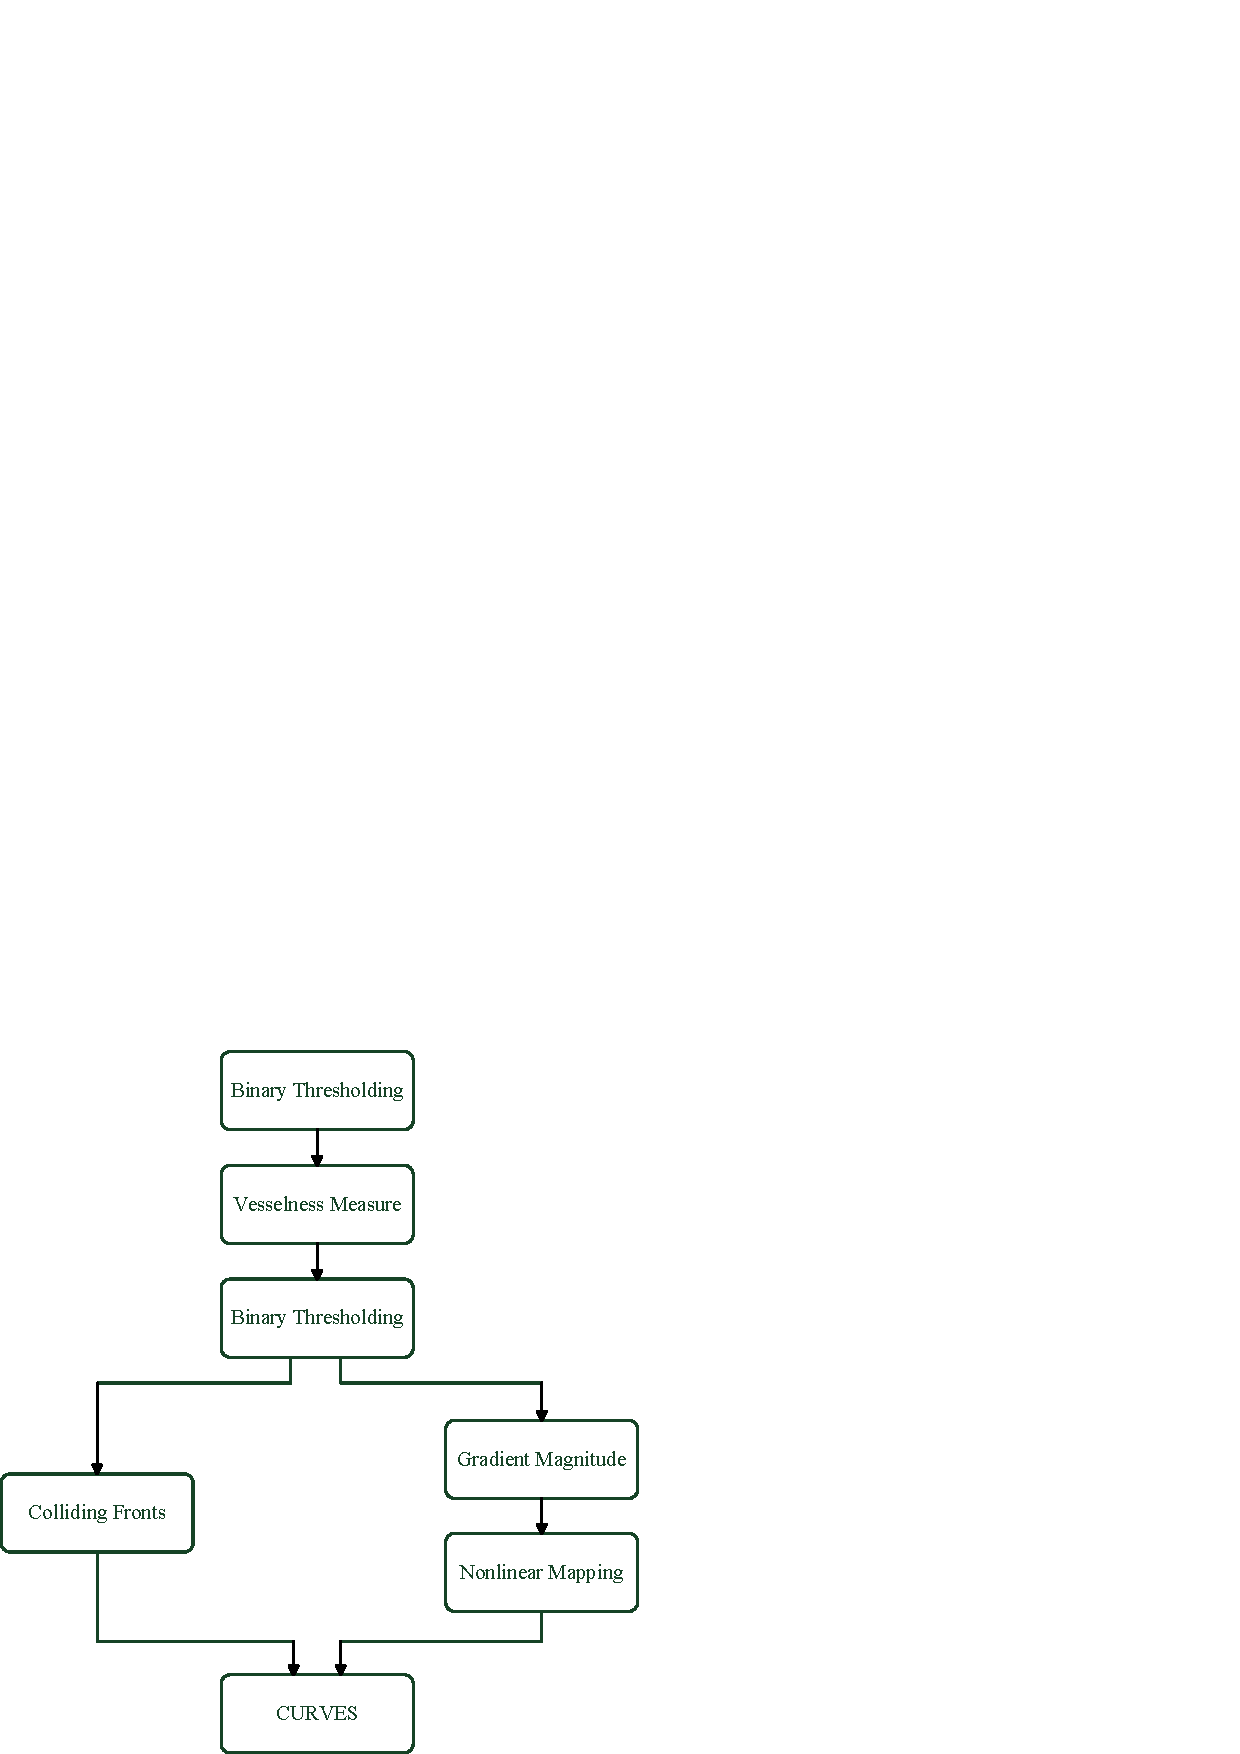
\includegraphics[height=3.2in,width=3.2in]{Figures/chap04/DataFlow.png}
\caption{Collaboration diagram of the segmentation pipeline.}
\label{fig:DataFlow}
\end{figure}

\subsection{Tubular Objects Enhancement}

The tubular enhancement is a sort of multi-scale line filtering, whose scheme can be summarized as the ``tube-like" objects in the image are highlighted whilst the rest are attenuated. %
To achieve this, the three dimensional multi-scale algorithm proposed by Sato \textit{et al.} \cite{Sato1998} is introduced.

To shape the filter response to certain width of lines and suppress the noisy effects, the pixels need to convolving with the second order derivatives of a Gaussian kernel.
This computation is an equivalent to the calculation of the Hessian matrix $\mathcal{H}$ of the three-dimensional image $I(\cdot)$:
\begin{gather}
\label{eqn:Hessian}
\mathcal{H} = \nabla^2 I =
\begin{bmatrix}
I_{xx} & I_{xy} & I_{xz} \\ I_{yx} & I_{yy} & I_{yz} \\ I_{zx} & I_{zy} & I_{zz}
\end{bmatrix},
\end{gather}
where $I_{xx} = \frac{\partial^2 I}{\partial^2 x}$, $I_{xy} = \frac{\partial^2 I}{\partial x \partial y}$, to name a few.
And all these partial second order derivatives are the convolutions with the second order derivatives of a Gaussian kernel $G(x; \sigma)$ with the standard deviation $\sigma$:
\begin{equation}
\label{GaussianConvolution}
I_{xx} = I \ast \frac{\partial^2 G}{\partial^2 x}.
\end{equation}
The eigenvalues of (\ref{eqn:Hessian}) are $\lambda_1$, $\lambda_2$, and $\lambda_3$ with their values in descending order.
Their associated eigenvectors are $e_1$, $e_2$, and $e_3$, respectively.

When $\lambda_1 \approx 0$ and $\lambda_2 \approx \lambda_3 \ll 0$, the line measure can be written as
\begin{equation}
\label{eqn:LineMeasure}
\lambda_{123} =
\begin{cases}
\left| \lambda_3 \right| \left( \frac{\lambda_2}{\lambda_3} \right)^{\gamma_{23}} \left( 1 + \frac{\lambda_1}{\left| \lambda_2 \right|} \right)^{\gamma_{12}}, & \lambda_1 \le 0 \\
\left| \lambda_3 \right| \left( \frac{\lambda_2}{\lambda_3} \right)^{\gamma_{23}} \left( 1 - \alpha \frac{\lambda_1}{\left| \lambda_2 \right|} \right)^{\gamma_{12}}, & \frac{\left| \lambda_2 \right|}{\alpha} > \lambda_1 > 0 \\
0, & \text{otherwise}.
\end{cases}
\end{equation}
In (\ref{eqn:LineMeasure}), the additional parameters $\gamma_{12}$, $\gamma_{23}$, and $\alpha$ are all positive constant, where $\gamma_{12} \in [0, \infty)$ is used to discriminate between the branching structures and the noises as well as pseudo-branches, $\gamma_{23} \in [0, \infty)$ regulates the sharpness, and $\alpha \in (0, 1.0]$ maintains the asymmetrical characteristics of the last terms of the function for all possible $\lambda_1$.

Additionally, different choices of the eigenvalues can equip the line filter with the abilities in detecting different shapes of the objects as shown in Table. \ref{tbl:Eigenvalues}. %

\subsection{Preprocessing for Level Set Evolution}

\subsubsection{Speed Images Calculation}

Level set algorithms evolves the contours in the gradient field with ``sharp" variations in intensity values from the inner or outer area to the boundaries.
The aim of the speed images is to provide this gradient field in the form of nicely shaped gradient images.
In the gradient images, the magnitude of the gradient at each pixel is calculated.
Next the gradient images $I_{\nabla}$ are transformed into the speed images $I_{\sigma}$ by applying the nonlinear relation:
\begin{equation}
\label{eqn:Sigmoid}
I_{\sigma} = (I_{max} - I_{min}) \cdot \frac{1}{1 + \exp\left(-\frac{I_{\nabla} - n}{m}\right)} + I_{min},
\end{equation}
where $I_{max}$ and $I_{min}$ are the two extreme values of the output intensity values, $m$ is a constant that controls the window width of the input intensity, and $n$ is a constant that defines the center of the window.
\begin{table}
\renewcommand{\arraystretch}{1.3}
\caption{Eigenvalue sets for detecting different shapes}
\label{tbl:Eigenvalues}
\centering
\begin{tabular}{l||c}
\hline
\bfseries Shape & \bfseries Eigenvalues \\
\hline\hline
Bright tubes   & $\lambda_1 \approx 0, \lambda_2 \approx \lambda_3 \ll 0$ \\
Dark tubes     & $\lambda_1 \approx 0, \lambda_2 \approx \lambda_3 \gg 0$ \\
Bright plates  & $\lambda_1 \approx \lambda_2 \approx 0, \lambda_3 \ll 0$ \\
Dark plates    & $\lambda_1 \approx \lambda_2 \approx 0, \lambda_3 \gg 0$ \\
Bright spheres & $\lambda_1 \approx \lambda_2 \approx \lambda_3 \ll 0$ \\
Dark spheres   & $\lambda_1 \approx \lambda_2 \approx \lambda_3 \gg 0$ \\
\hline
\end{tabular}
\end{table}

\subsubsection{Initial Contours Evolution Using Colliding Fronts}

The aim of the colliding fronts module is to evolve the contours for the CURVES system from the user-defined seeding points.
The colliding fronts method is implemented based on the principles of the fast marching algorithm \cite{Sethian1999}.
However, this method requires two seeds for each round of evolution such that the area between the seeds can be extracted.
The output of this module is the dot production of the gradient field of arrival times of the two wavefronts.
The level set initialization for the prolonged objects greatly benefit from this feature of the method.
On the other hand, the method also shortens the computation time.

\subsection{CURVES Evolution Model}

The CURVES method \cite{Lorigo2001} is chosen as the functioning segmentation method because of the complex nature of the coronary arteries.
It is highly effective in the segmentation of the complicated curvilinear structures in the volumetric medical images.
In addition, the criterion of CURVES method also takes the local smoothness of the boundaries to be detected (i.e., the inner wall of the coronary arteries) into account.

This method is a modification of the geodesic active contours method developed in Caselles \textit{et al.} \cite{Caselles1997}.
As the extensive research of the geodesic active contours, CURVES is a level set algorithm that models the tiny vessels as spatial curves with arbitrarily complicated topology \cite{Lorigo2001}. %
CURVES evolves the level sets to the boundaries of the targets based on the criterion of the minimization of the following energy functional
\begin{equation}
\label{eqn:CURVES}
\oint_0^1 g\left( \left| \nabla I \left( \mathcal{C} \left(  s \right) \right) \right| \right) \left| \mathcal{C}'\left( s \right) \right| ds,
\end{equation}
where $\mathcal{C}\left( s \right): [0,1] \rightarrow \mathrm{R}^3$ is a one-dimension curve, $I\left( \cdot \right): [0, a] \times [0, b] \times [0, c] \rightarrow [0, \infty)$ is an image on which the curve evolution takes place, and $g\left( \cdot \right): [0, \infty) \rightarrow \mathrm{R}^+$ is a monotonically decreasing function. %

The minimization of this functional can be achieved by searching for the gradient descent direction of the functional itself, which means the Euler-Lagrange equations associated with (\ref{eqn:CURVES}) needs to be computed. %
Thus the geodesic flow equation that controls the contour evolution in this process of minimization can be obtained as follows
\begin{equation}
\label{eqn:Evolution}
\frac{\partial \mathcal{C}}{\partial t} = k \mathcal{N} - \frac{g'}{g} \varPi \left( \mathcal{H} \frac{\nabla I}{ \left| \nabla I \right| } \right),
\end{equation}
where $\mathcal{H}$ is the Hessian matrix of the image $I$, $k$ is the Euclidean curvature, $\mathcal{N}$ is the unit normal vector, $\varPi(\cdot)$ is the projection operator projects the argument onto the normal space. %
The update equation can be obtained as
\begin{equation}
\label{eqn:Update}
\frac{\partial v}{\partial t} = \mathcal{F} \left( \nabla v(x, t), \nabla^2 v(x, t) \right) + \frac{g'}{g} \nabla v(x, t) \mathcal{H} \frac{\nabla I}{ \left| \nabla I \right| },
\end{equation}
where $v(\cdot): \mathrm{R}^3 \rightarrow [0, \infty)$ is the embedding function of the curve $\mathcal{C}$, $\mathcal{F} \left( \nabla v(x, t), \nabla^2 v(x, t) \right)$ is the smaller eigenvalue of the matrix $P_{\nabla v} \nabla^2 v P_{\nabla v}$. %
The matrix $P_q$ is defined as a projector which projects some vector onto the normal plane of vector $q \in \mathrm{R}^3$:
\begin{equation}
\label{eqn:ProjectionOperator}
P_q = I_0 - \frac{qq^T}{\left| q \right|^2},
\end{equation}
where $I_0$ denotes the identity matrix.

By incorporating the speed images $I_{\sigma}$ to the evolution equation (\ref{eqn:Evolution}), the evolution in our case can be obtained as
\begin{equation}
\label{eqn:Application}
\frac{\partial \mathcal{C}}{\partial t} = k \mathcal{N} - \frac{g'(I_{\sigma})}{g(I_{\sigma})} \varPi \left( \mathcal{H} \frac{\nabla I_{\sigma}}{ \left| \nabla I_{\sigma} \right| } \right).%
\end{equation}

\subsection{Surface Rendering}

The surface information is extracted for the visualization by the marching cubes method \cite{Lorensen1987MC}.
Cubes are created based on the input information and are organized into an array structure.
Each cube consists of eight pixels (each four pixels are from a slice).
The index of each cube is labeled by comparing the intensity values of every pixel to the isovalue of the surfaces.
Next the patterns of the intersection between objects and cubes are initially determined based on the triangulated cases.
Then the precise intersection are computed using linear interpolation with the intensity values at each vertex.
The unit normals to the surface are calculated via central differences for the vertices of the cubes.
Finally the generated triangles are ready for the surface rendering.

\section{Experiments and Results}

\subsection{Medical Data and Experimental Setup}

The original chest CTA series was acquired by a 128-slice Siemens SOMATOM Definition Flash CT.
The slice thickness was $0.6 \text{mm}$ and the in-slice resolution was $0.4 \times 0.4 \text{mm}^2$.
Since the work was all on the coronary arteries, the volume contained the whole heart (i.e., ROI, which is the abbreviation of \textit{region of interest}) was cropped from the original data as shown in Fig. \ref{fig:Original}. %

Numbers of experiments were conducted with different sets of parameters to segment the coronary arteries from CTA for the testament of the approach in this paper.
In our case, the original CTA series in DICOM format had been converted to the form of XML first; and the data type of pixels are converted for the incoming computation.
Next the converted data was enhanced by the module which was implemented based on the algorithm developed in \cite{Sato1998}.
Then the tubular enhanced data was send to the following modules to perform calculations of speed image production and input level sets generation.
The two set of the resulting data from the two computation pipelines were transferred to the CURVES module in order to generate the final fronts evolution results.
Finally, the marching cubes method was employed to extract the iso-surface corresponding to the wall of the coronary arteries.
All the experiments were performed on a machine with Intel's 2.83GHz Core 2 Quad CPU and 4GB RAM.

\subsection{Tubular Enhancement and Its Postprocessing}

Before the tubular enhancement started, a global binary thresholding was performed in order to provide the enhancing filter with the focus on the tiny bright tubular objects.
To achieve this, the thresholder was called to trim the irrelevant contents in the images, e.g., dark lung regions with negative intensity values, bright bone regions with large positive intensity values, etc. %
As shown in Fig. \ref{fig:Binary1}, the intensity values of the regions within the interval between the lower threshold and the upper threshold were uniformly assigned a unique intensity value, i.e., $255$ in our case; the intensity values of the rest regions were uniformly assign a zero intensity value. %

Referring to the shape prior guidelines listed in Table. \ref{tbl:Eigenvalues}, the tubular enhancement filter was fed the parameters to detect the bright tubular objects, i.e., coronary arteries. %
Among these parameters, $\sigma$ controls the diameter of cross-section of the tubular objects to be enhanced, $\gamma_{12}$ is the measure of the tube similarity, and $\gamma_{23}$ is used for the recovery of vessel regions with inhomogeneous contrast or intensity loss. %
As shown in Fig. \ref{fig:Vesselness}, the tiny vessels including the coronary arteries and the vessels in lung areas were enhanced with a small $\sigma$ whilst the tubular structures with cross-section diameters larger than this value were not enhanced. %

The intensity values of the enhanced tubular objects were relatively low and scattered in a wide range.
This is a mass for the selection of the intensity value in the following processing steps.
To deal with it and facilitate this situation, some intensity transformation step was needed.
The nonlinear intensity mapping filter and the binary threshold filter were the candidates.

Equation (\ref{eqn:Sigmoid}) showed that the nonlinear intensity mapping transformed the input image into the image with partial enhancement and partial attenuation.
With the well chosen parameters, the intensity values corresponding to the targeting objects in this case were enlarged and the rest part of the images in lower intensities were all depressed as near zero intensity areas. %
Because of the mapping characteristics of the sigmoid functions, the intensity values of the bright tubular structures were not uniformly distributed and stayed at the relatively low levels (see Fig. \ref{fig:Sigmoid}). %
In another test, the binary threshold filter extracted the pixels with the intensities in the specified range and assigned them with a unique large intensity value as discussed above (see Fig. \ref{fig:Binary2}). %
Comparing the result of the two candidates, the binary threshold filter was selected to improve the results of the precedent tubular enhancement filter (see Fig. \ref{fig:DataFlow}). %
\begin{figure}[t]
\centering
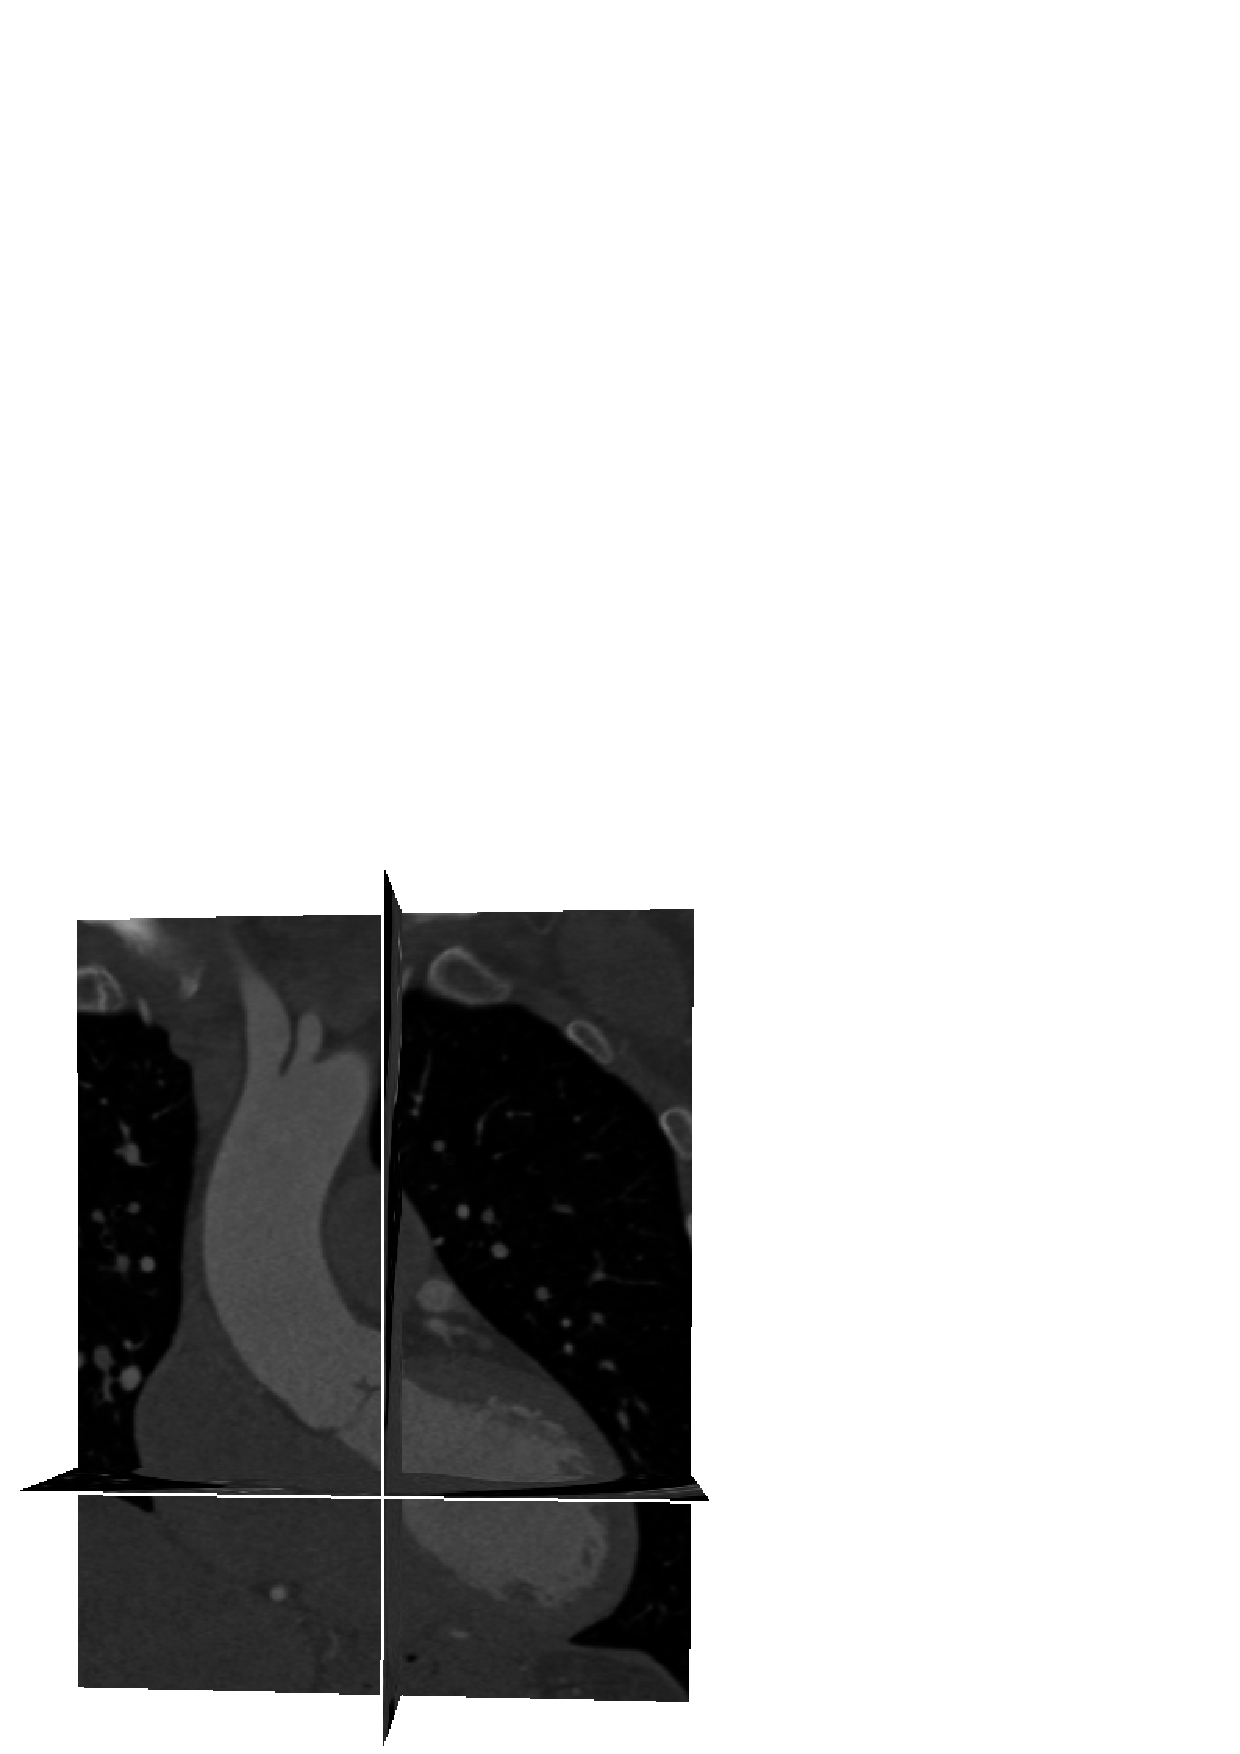
\includegraphics[width=2.8in]{Figures/chap04/original.png}
\caption{Original ROI-extracted volumetric data}
\label{fig:Original}
\end{figure}
\begin{figure}[t]
\centering
\subfloat{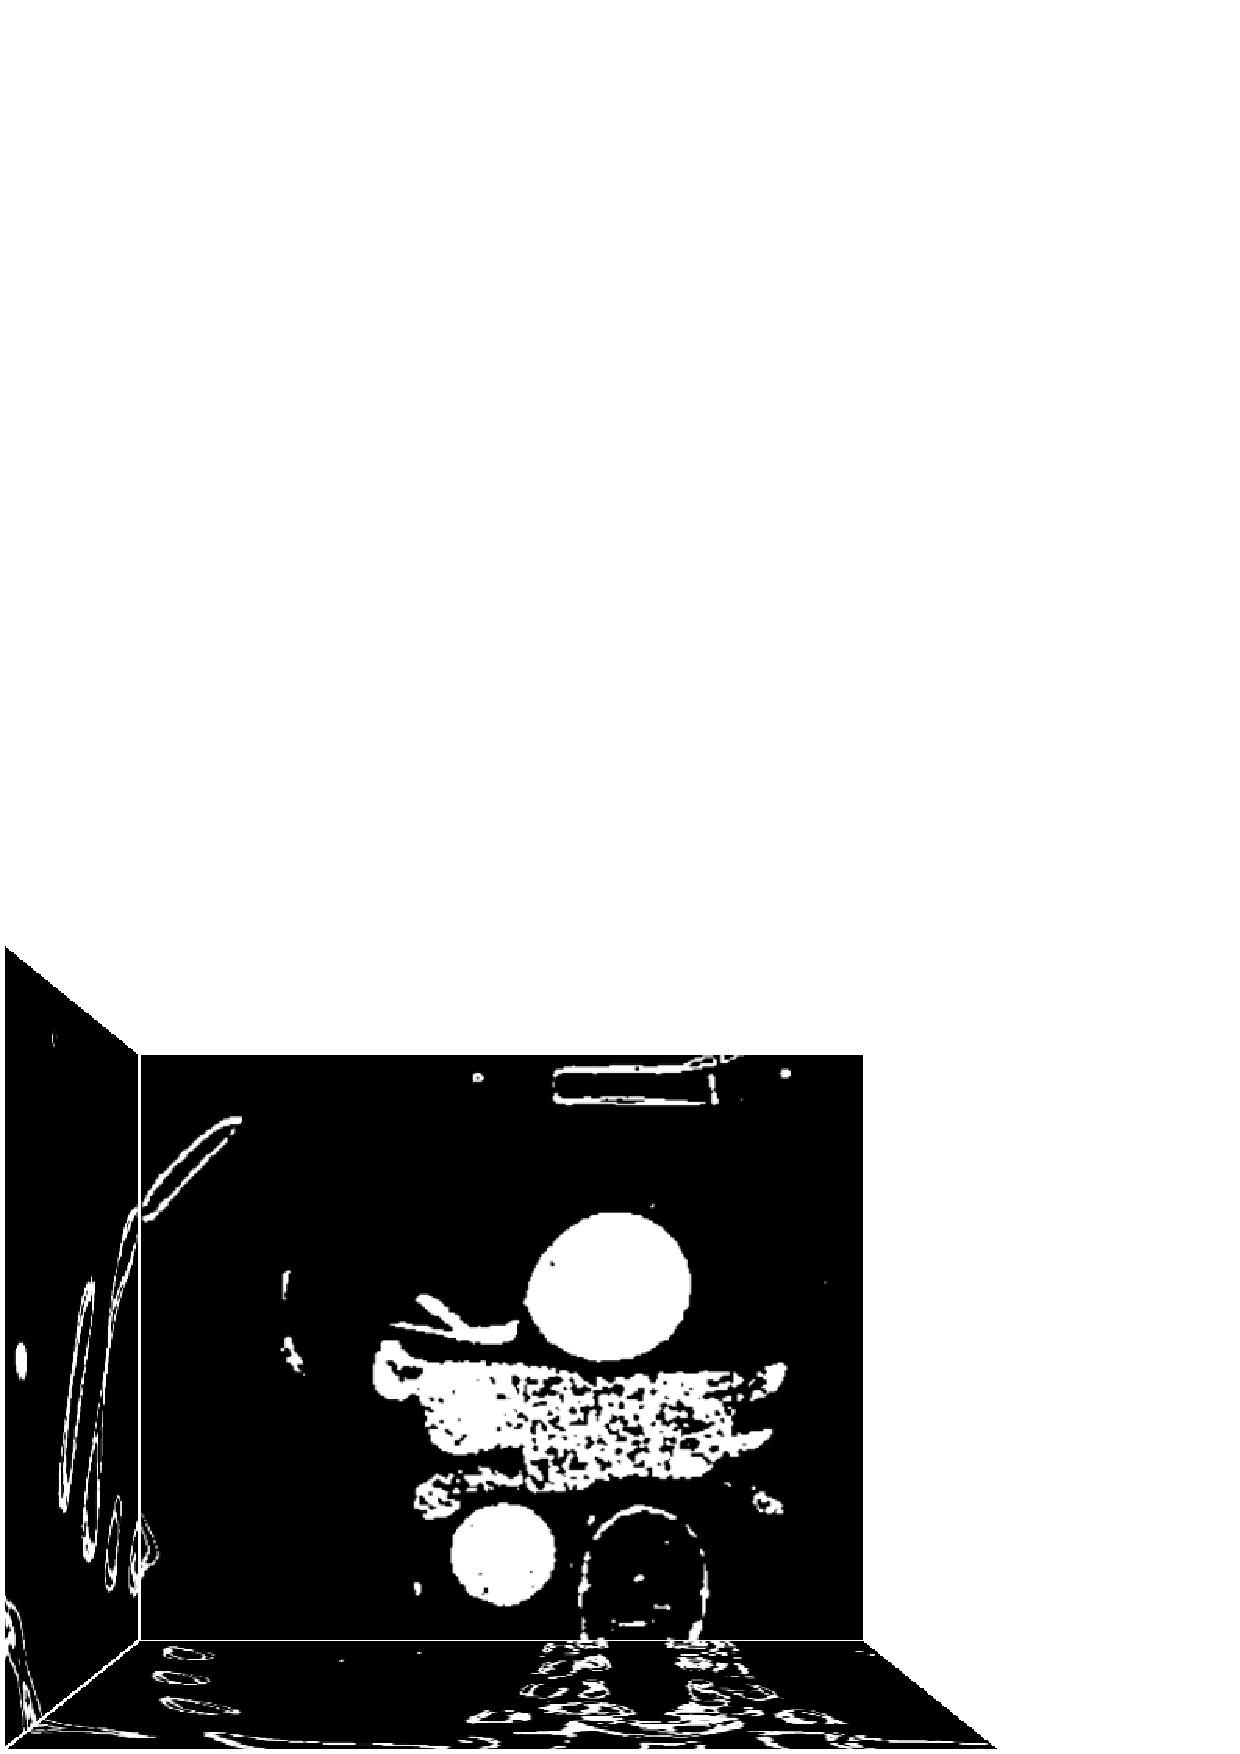
\includegraphics[width=2.8in]{Figures/chap04/binary1.png}%
\label{fig:Binary1}}
\hfil
\subfloat{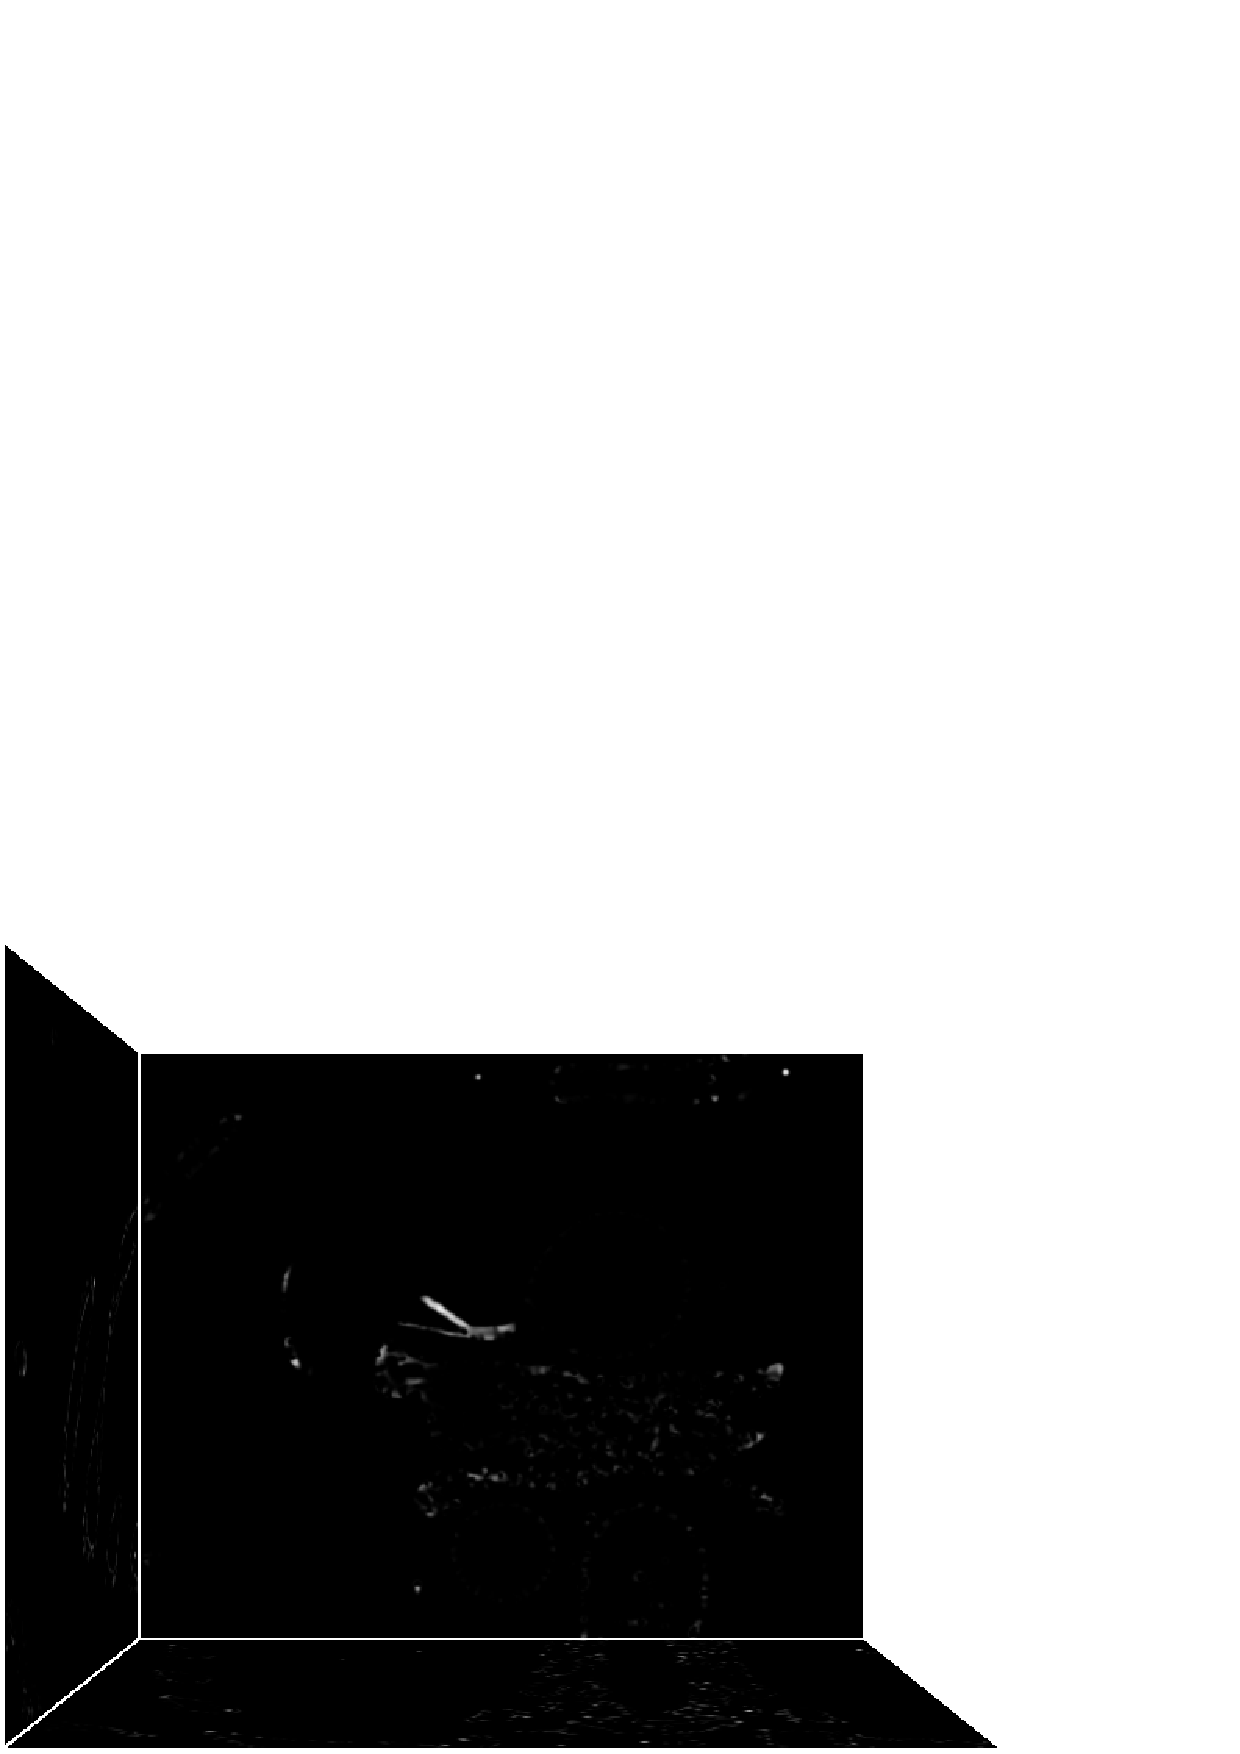
\includegraphics[width=2.8in]{Figures/chap04/hessian.png}%
\label{fig:Vesselness}}
\caption{Preprocessing results of the original CTA images based on the ``vesselness" measure: (a) binary thresholding ($\text{lower threshold} = 300$, $\text{upper threshold} = 600$) (b) tubular enhancement ($\sigma = 0.9$, $\gamma_{12} = 0.1$, $\gamma_{23} = 2.0$).}%
\label{fig:Preprocessing}
\end{figure}

\subsection{Feature Images Computation}

To generate the feature images for the CURVES system, two steps were performed:
(1) calculating the gradient magnitude at each pixel; and
(2) converting the gradient images into the speed images.
%\begin{enumerate}
%\item calculating the gradient magnitude at each pixel;
%\item converting the gradient images into the speed images.
%\end{enumerate}
The gradient magnitude module computed the magnitude of the gradient pixel-wisely for the image by performing the convolution with the first order derivatives of a Gaussian kernel.
The wall of the tiny vessels were extracted before the nonlinear intensity mapping was employed to generate the edge potential maps.
The extreme values of the pixel intensities in the gradient magnitude images directly effected the selection of the parameters in (\ref{eqn:Sigmoid}).
To reverse the lightness of the objects (in low intensities in the gradient magnitude images) and its edges (in high intensities in the gradient magnitude images), $n$ was chosen to be the center of the intensity window containing the vessels, and $m$ a negative value with $|m|$ as the width of the window. %
The minus sign of $m$ means the reverse operation on the pixels.
The neighborhood of the boundaries of the objects were in almost zero intensity, which made the evolution driven by (\ref{eqn:Application}) faster in the ``plateau" (with uniformly high intensities), whilst much slower (in a speed of about zero) in the ``ridges" (with rapid decreasing intensities). %

\subsection{Wave Fronts Propagation}

The initial level sets were evolved by the colliding fronts module.
Two seeds were located interior of the regions corresponding to the coronary arteries and the interfaces surrounding each seeds evolved towards each other.
The dot production of the gradients of arrival times of the two wavefronts were computed.
\begin{figure}[t]
\centering
\subfloat{
\includegraphics[width=2.8in]{Figures/chap04/sigmoid.png}%
\label{fig:Sigmoid}}
\hfil
\subfloat{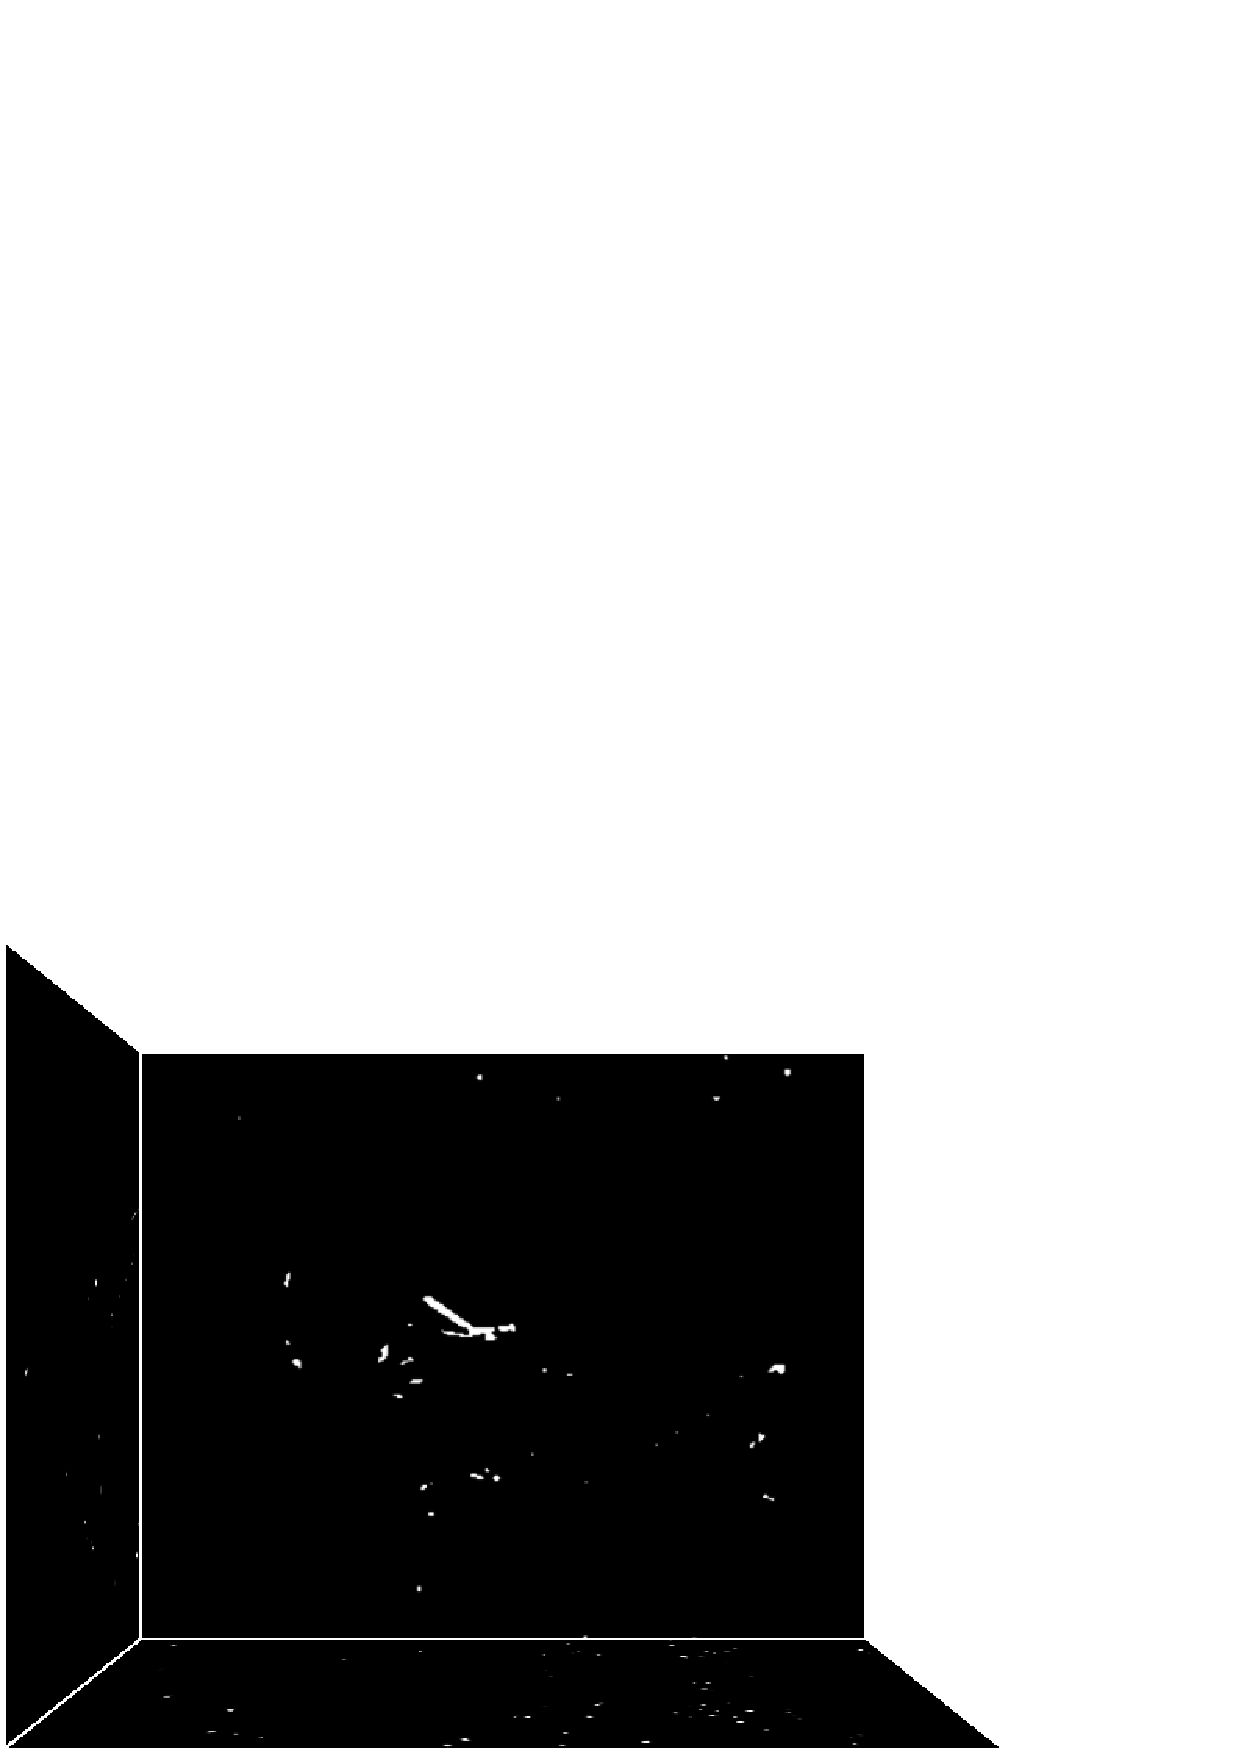
\includegraphics[width=2.8in]{Figures/chap04/binary2.png}%
\label{fig:Binary2}}
\caption{Comparison of the two different intensity conditioning approaches: (a) nonlinear intensity mapping ($m = 80$, $n = 120$); (b) binary thresholding ($\text{lower threshold} = 40$, $\text{upper threshold} = 200$).}%
\label{fig:IntensityConditioning}
\end{figure}
\begin{figure}[t]
\centering
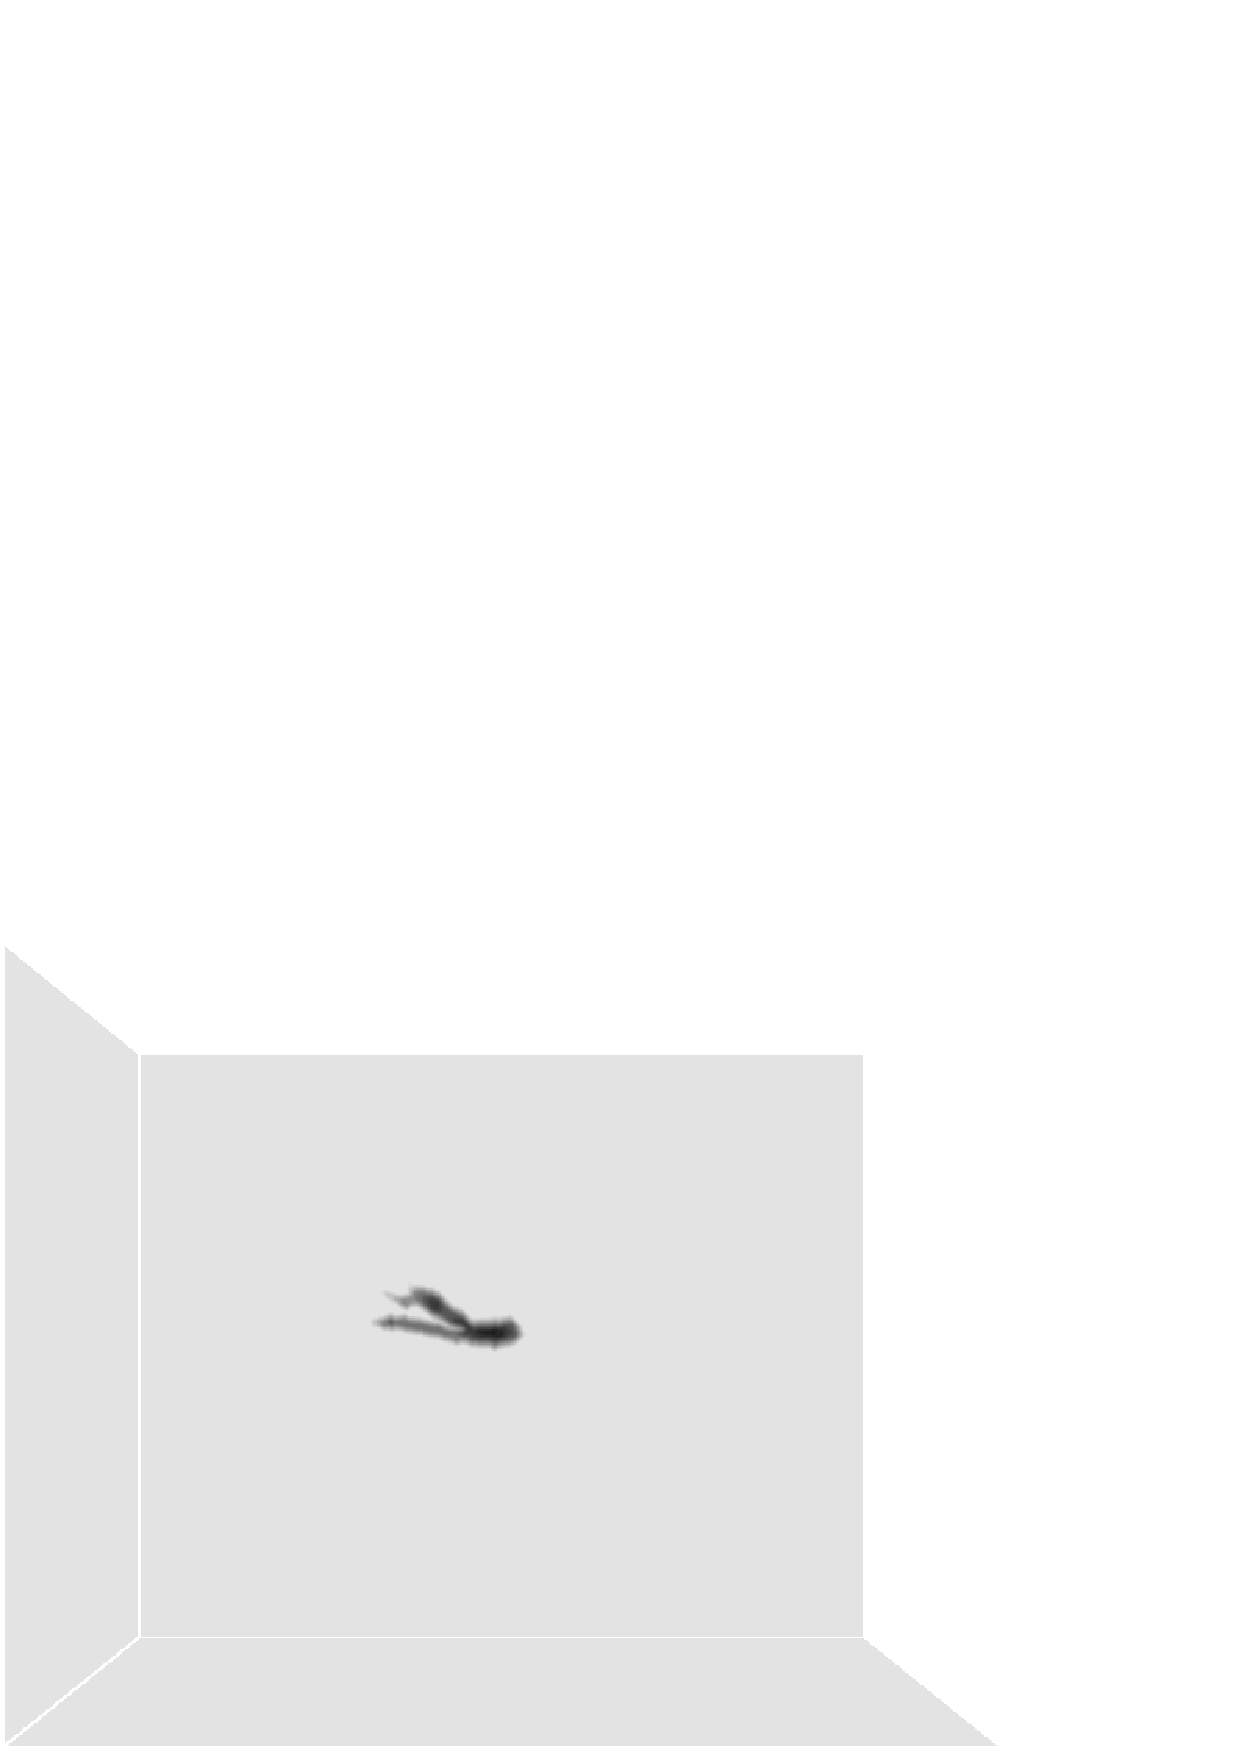
\includegraphics[width=2.8in]{Figures/chap04/curves.png}
\caption{CURVES evolution based on the initial contours generated by the colliding fronts method and the edge feature maps calculated by the nonlinear intensity mapping function.}%
\label{fig:CURVES}
\end{figure}
\begin{figure*}[t]
\centering
\subfloat{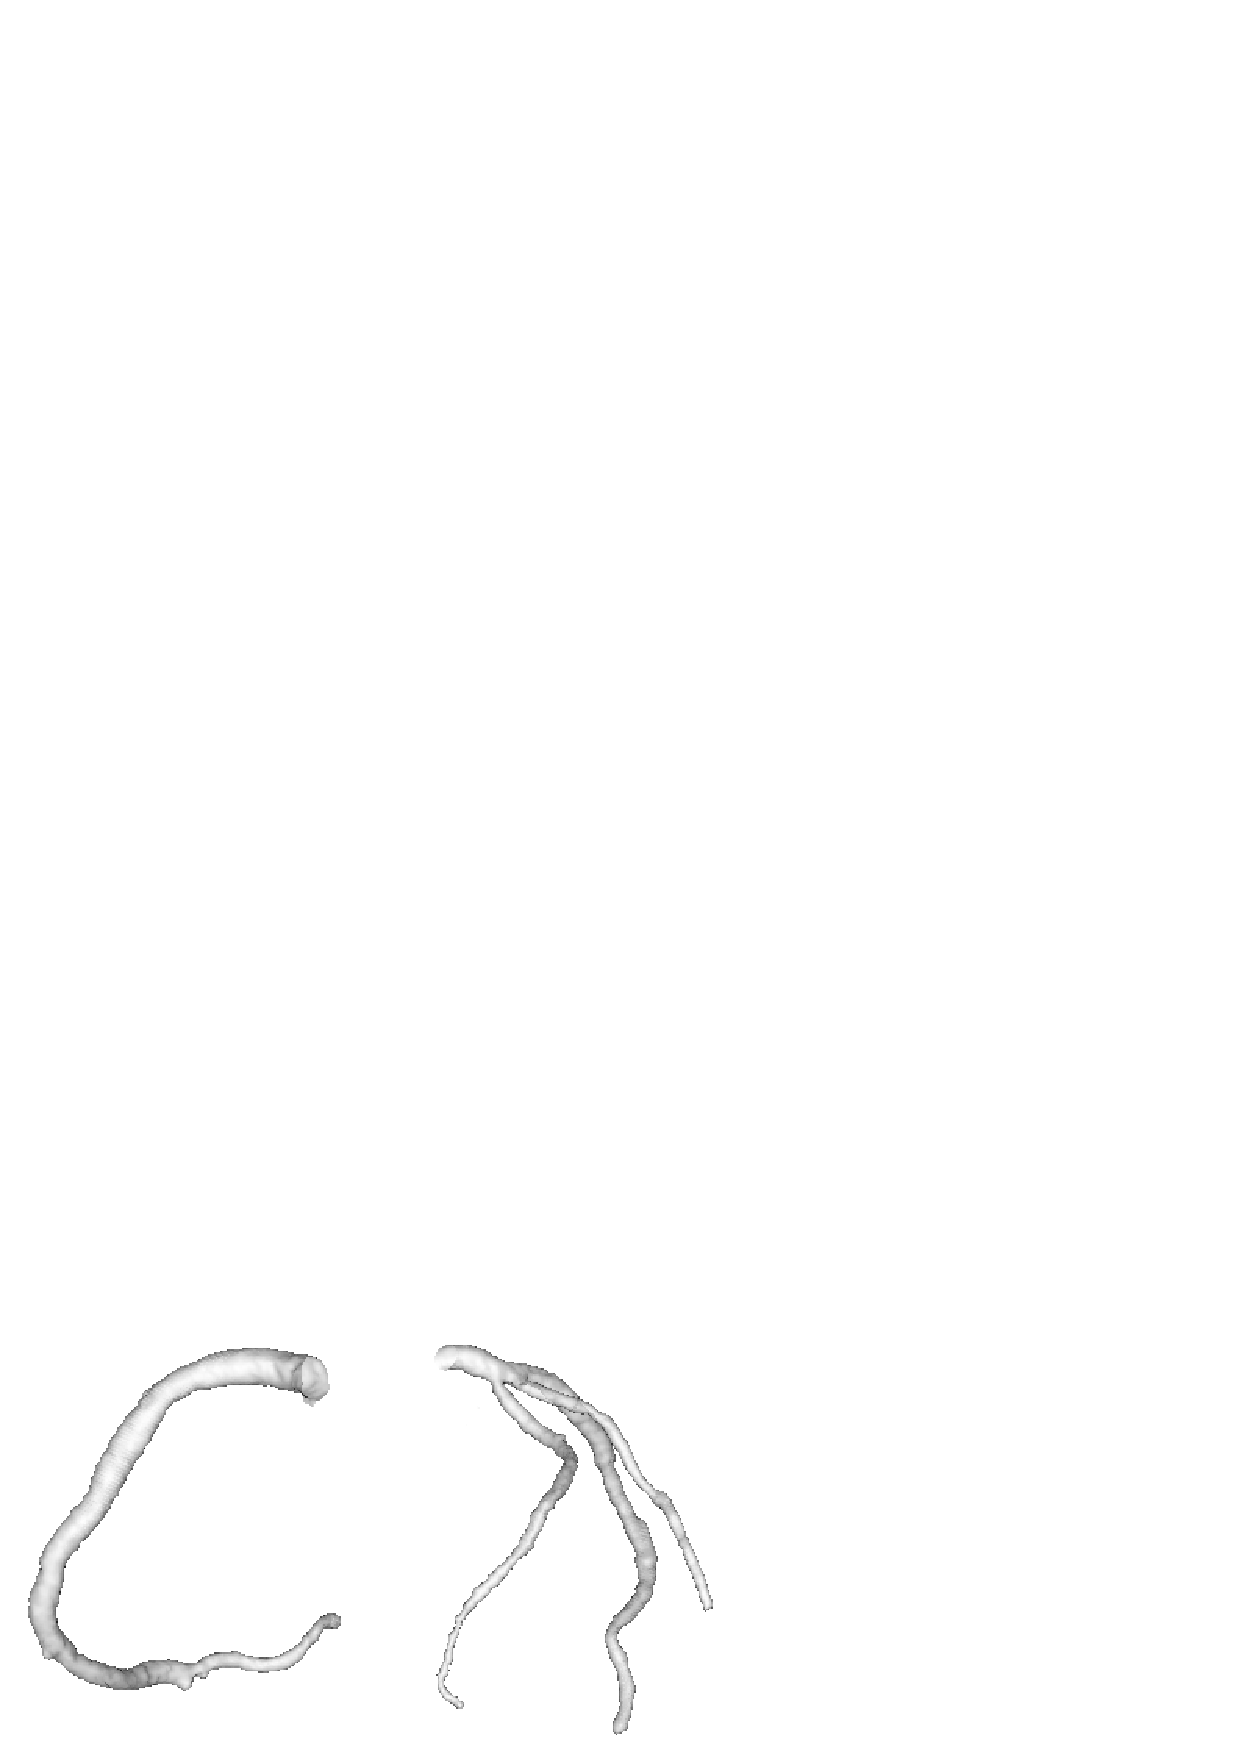
\includegraphics[width=2.8in]{Figures/chap04/model_conventional.png}%
\label{fig:VisualizationModelCURVES}}
\hfil
\subfloat{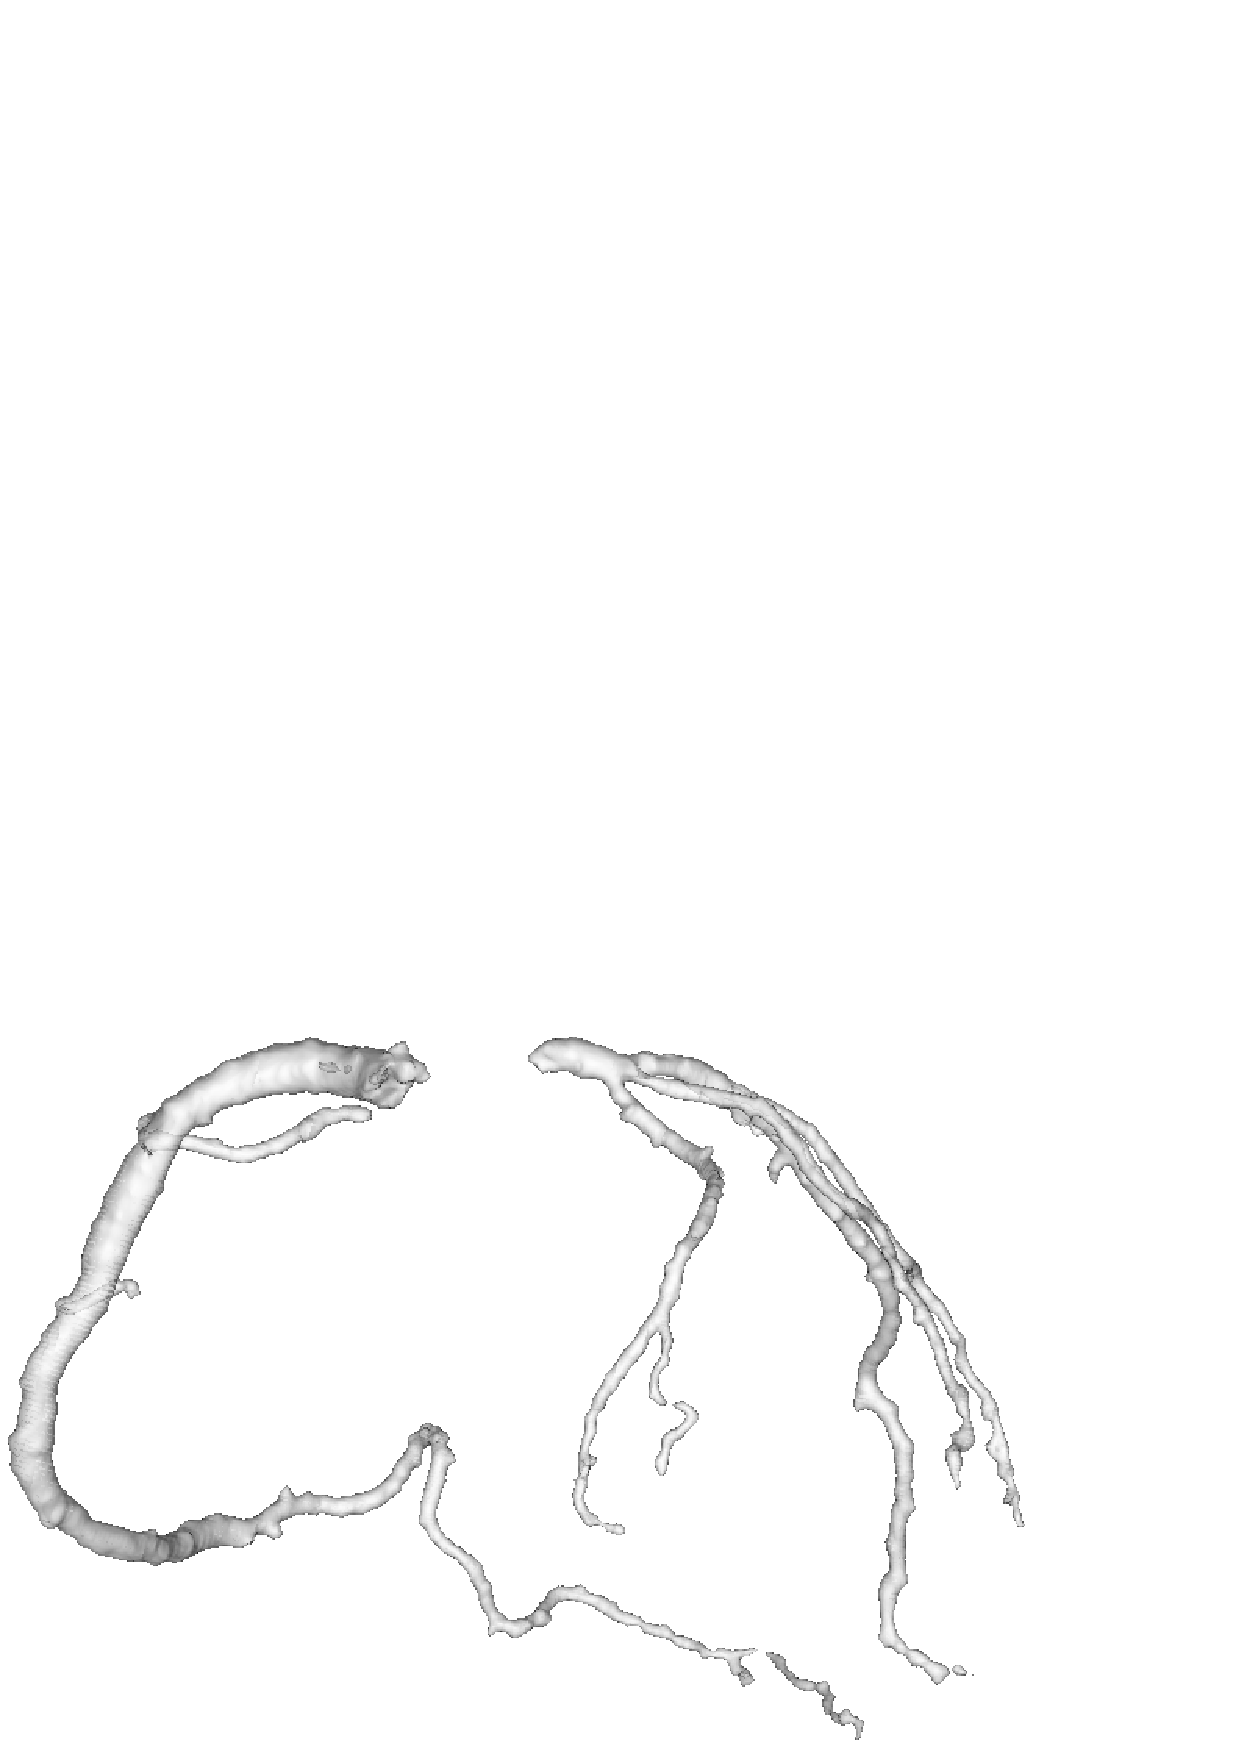
\includegraphics[width=2.4in]{Figures/chap04/model_enhanced.png}%
\label{fig:VisualizationModelTECURVES}}
\caption{Models of the coronary arteries: (a) conventional CURVES evolution; (b) tubular-enhanced CURVES evolution.}%
\label{fig:VisualizationModel}
\end{figure*}

The CURVES system started working when all the preceding calculation completed.
The module took the speed images as its evolution maps and the initial contours as its initial states and regulates the evolution according to (\ref{eqn:Application}).
The evolution terminated when the contours evolved against the wall of the coronary arteries in the specified steps of iterations.
And the resulting evolution extracted the coronary arteries as shown in Fig. \ref{fig:CURVES}.
Next a binary thresholding step was provoked to label the inner area of the coronary arteries with high intensity value whilst the outer area with zero intensity value.

\subsection{Visualization of Segmentation Results}

By manually picked the isovalue corresponding to the wall of the coronary arteries, the resulting volume were processed using the marching cubes method \cite{Lorensen1987MC}.
The visualization models of the coronary arteries respectively based on the CURVES regions without and with tubular enhancement demonstrated their capabilities of displaying the complicated geometrical details (see Fig. \ref{fig:VisualizationModelCURVES} and \ref{fig:VisualizationModelTECURVES}). %

\section{Conclusions and Future Work}
%The conclusion goes here.

The three dimensional visualization of the blood vessels plays an important role in the construction of the virtual scenario for the robotic surgical simulator.
Further, the visualization of the coronary arteries is the most critical and difficult work.
Because of the complex spatial topologies, details can be easily lost in the process of segmentation.
In this paper, a vasculature segmentation method based on tubular-enhanced CURVES has been developed.
Then the process of the experiment was presented and the results were demonstrated.
The experimental results showed that the proposed approach is capable of enhancing the tiny dark vessels and visualizing the geometric details of them.

The tubular feature of coronary arteries was enhanced and the speed images were generated.
Meanwhile, the initial contours for the CURVES method were computed by a modified version of fast marching method in another process.
The actual level sets evolution began after the above computation finished and the evolution took a specified number of iterations to detect the coronary arteries.
At the end of the segmentation, the resulting pixels were all conversed in their intensities.
Finally the data representing the surface of the arteries was extracted by the marching cubes method.

Our future plans are the further optimization of the blood vessel models for the simulation with virtual tools of the robotic surgical simulator.
The principle work will be the decimation of the quantity of the triangles consisting the blood vessels and the improvements of the visualization effects of the virtual scenario. 
%# -*- coding:utf-8 -*-
\chapter{血管模型中心线的提取}
\label{chap7}

\section{Introduction}
% no \PARstart
Cardiovascular diseases are among the most fatal illnesses worldwide \cite{WHO2013}.
The diseases occur when the stenosis or even blockages formed due to the build up of fatty substances on the inner wall of the blood vessels.
Percutaneous coronary intervention (PCI) is the gold standard in fighting the lethal diseases.
Due to its minimally-invasive nature, this procedure only causes small incision and much less trauma to the patients.
In addition, the hospitalization after the procedure is in turn dramatically shortened.
However, due to the very nature of minimally-invasiveness of PCI and the complex anatomic structure of the blood vessels, the learners need thorough and strict training before performing the procedure in action. %
What's worse, the practitioners in catheterization labs have to expose themselves under the ionizing radiation from the fluoroscope while examining the morphologies of the patients' vasculature. %

The surgical robotic systems for intravascular procedures have greatly changed this situation.
With the assistance of the robotic systems, cardiology practitioners need not to be worried about the radioactive exposure and the relative risks any more.
Like their ancestors (i.e., the traditional PCI procedure), the skills of manipulating the robotic system to do the surgery are also not easy for the junior residences and still require strict and sufficient training before applying the procedure on the real patients. %

The traditional ways of training PCI procedure are deeply rooted in the physical fashion, i.e., employing biological models (e.g. human cadavers and living animals) or non-biological models (e.g. phantoms). %
The former are disposable and ethic-disputed; let alone the tremendous expenditure on the preservation and feeding, and the distinction in anatomy between human and animal volunteer. %
The latter are stiff and lack of sufficient anatomic details, even though they can be used repeatedly.
Indeed, it is infeasible to conduct the training on the expensive robotic systems whilst ignoring the real needs in the catheterization labs.
To streamline the training and the practice of robotic PCI procedure, a well-designed computing simulation system is required.

The aim of our effort is to provide a training tool of convenience and effectiveness for the minimally-invasive intravascular robotic system \cite{Ji2011EMBC}.
In constructing this training vehicle, the anatomic structures in computing environment especially the vascular system are definitely one of the most substantial components.
The centerlines is an effective way of describing the shape of the model \cite{Ogniewicz1995}, which will provide accurate shape description for the path planning in interactive simulation.
In this paper, we developed an automatic approach based on the Voronoi diagram \cite{Antiga2003} to extract the centerlines of the vasculature.
The input of the proposed approach is the patient-specific image-based surface model of the vasculature, which is reconstructed by applying our previous work \cite{Yang2014ICRA}. %
Before computing the Voronoi diagram of the tubular surface model, several preprocessing should be performed.
First, the connectivity of the polygons that consisting the surface is validated thoroughly to include the largest connected polygons that is effective in representing the surface. %
Second, the bumpy and crusty surfaces are smoothed in order to reduce the effects on the computation of centerlines.
Third, the surfaces are subdivided to gain a more precise geometric feature.
Finally, the centerlines of the vessel model by solving the Eikonal equation in the fast marching flavor.
The capability of our approach in automatically extracting the centerlines of the vessel model is proved by the experimental results.

The rest of this paper is organized as follows.
Section II introduces the related work of the centerline extraction methods for three dimensional objects.
Section III outlines the work flow and describes the techniques used in this work.
Section IV describes the experiments, ending with a brief discussion.
The final section concludes the whole work.

\section{Related Work}

Many researches have been done since the earliest work on extracting the centerline was proposed by Blum \cite{Blum1967}.
According to reference \cite{Ogniewicz1995}, most of these methods fall into four categories: (1) topological thinning; (2) distance transformation; (3) ``prairie fire" approach; (4) Voronoi Diagram methods. %

Topological thinning methods \cite{Ma2002,Sadleir2002} implement the centerline extraction by iteratively remove most of the ``simple points" except the ones that are the end-points of the generated centerline models. %
By ``simple points", it means that the boundary points consisting the object such that their removals do not destroy the topology of the object.

Distance transformation methods \cite{Niblack1992} find the centerline by searching the local maximum among the minimal distances between the points interior of the shape and the boundary. %
However, they do not ensure the resulting centerlines are connected with each other.

``Prairie fire" methods \cite{Blum1967,Leymarie1992} compute the centerline by determining the intersection of the propagating interfaces with their sources located on the boundary of the shape. %

Voronoi diagram method \cite{Sherbrooke1996,Antiga2003} treats the centerline to be generated as a subset of the Voronoi diagram.
These methods are sensitive to the noises and the regularization of the boundary of the shape.

There are numbers of other methods that are not belong to any category listed above.
Ferchichi and Wang in \cite{Ferchichi2006} reported a clustering-based algorithm for centerline extraction both for 2D and 3D objects.
The algorithm was designed based on the idea of computing the maximal disks/balls determining the centerlines, which is achieved by executing the K-means algorithm iteratively on the object-points and their distance transforms. %
Egger \textit{et al.} \cite{Egger2007} reported a centerline extraction algorithm for the blood vessels using Dijkstra's shortest path algorithm, which was designed for the catheter simulation. %

\section{Methodologies}

This section discusses the design of the processing pipeline and details the principles of the consisting modules.
Before the actual centerline extraction begins, several processing aims to removing noises and smoothing the irregular surfaces need to be run to guarantee the quality of the input surface.
The image-based surface model of the blood vessels needs series of postprocessing steps depicted in Fig. \ref{fig:DataFlow} to meet the requirements of the centerline computing module. %
Among these processing steps, the first one is the validation of the connectivity of the consisting polygons.
During this process, the largest possible connected regions of the surface model are extracted.
Next, the surface smoothing step is needed to depress the ``crusts" and ``stairs" in the surface.
Then the normal vectors (i.e., normals) are computed to mark the ``inside" and the ``outside" of the surface model.
After that, the consisting polygons need to be subdivided under a specified criterion to facilitate the computation of the centerline extraction at the cost of longer computation time. %

%\subsection{Processing on Image-Based Surface Model}

\subsection{Connectivity Validation and Largest Region Extraction}

In this paper, the vasculature surface model is generated from the original medical volumetric data set by applying the approaches reported in our previous work \cite{Yang2014ICRA}. %
In order to find the largest region spanning the surface of the vasculature, the connectivity among the vertices in the image-based surface model needs to be thoroughly validated at the beginning of the processing. %
The inner working is to extract consisting polygons that share common vertices and meet some requirements.
In the present paper we implement the algorithm to extract the largest connected region from the input surface.
\begin{figure}[t]
\centering
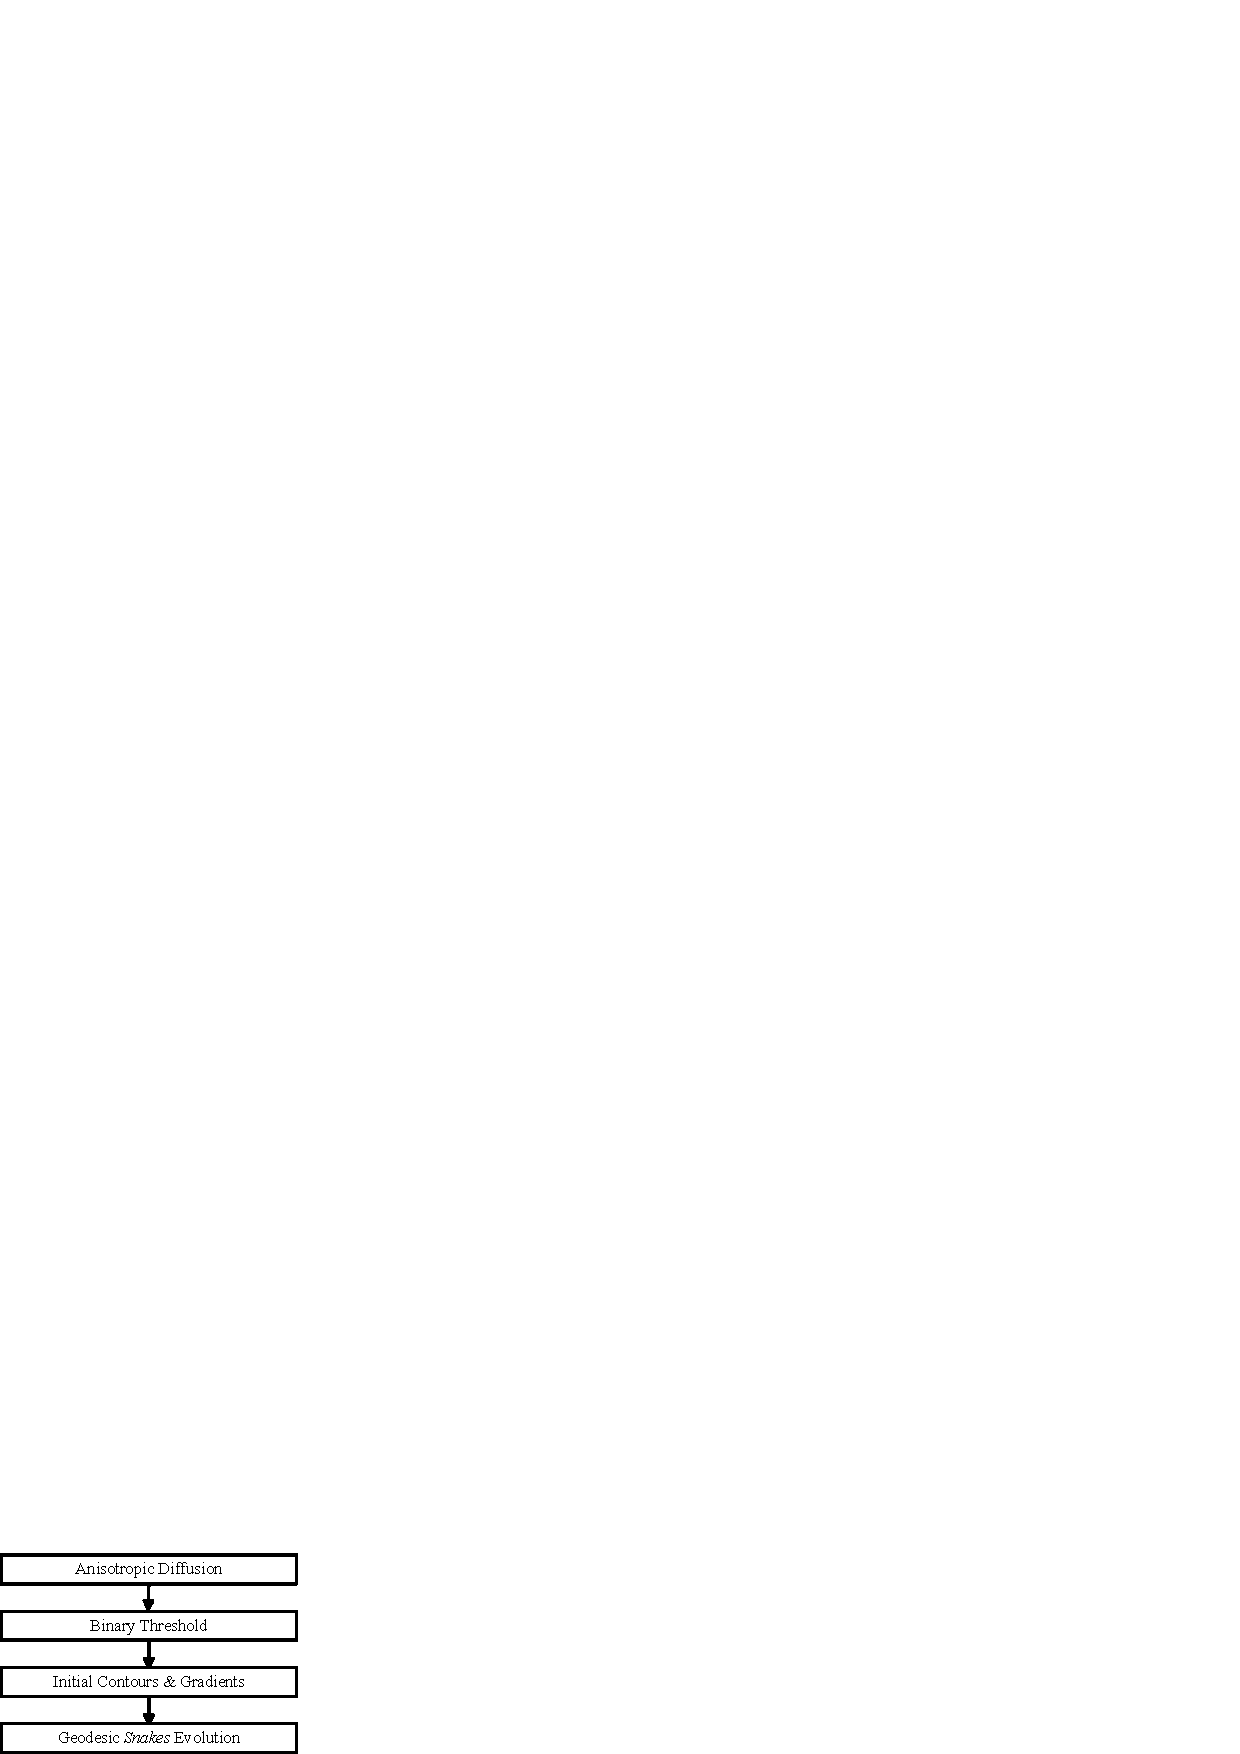
\includegraphics[width=3.2in]{Figures/chap05/DataFlow.png}
\caption{Overview of the work flow.}
\label{fig:DataFlow}
\end{figure}

\subsection{Surface Smoothing and Normals Computing}

There are plenty of methods used for the surfaces smoothing in visualization.
To overcome the ``facets" by-produced during this approximation, an optimal surface smoothing algorithm treating this problem as low-pass filtering by extending Fourier analysis is adopted \cite{Taubin1996}. %
The adopted method is built upon the formulation of the \emph{discrete graph signals}, which means the functions based on directed graph.
The directed graph $G$ represents the polyhedral surfaces in this problem, which is denoted as the set $\left\{ 1, \ldots, n \right\}$ of nodes with a set of neighborhoods $\left\{ i^{\ast}: i = 1, \ldots, n \right\}$ of node $i$. %
A discrete graph signal can be represented as a vector $x = \left[ x_1, \ldots, x_n \right]^T$, where each component of the vector corresponds one node of the graph.
A polyhedral surface $S = \{ V, F \}$ of $n$ vertices can be treated as a directed graph, where the vertices $V$ corresponds the set of nodes $n$ and the faces $F$ the polygons formed by connected nodes. %

The discrete surface signal, the discrete graph signal defined on the associated graph, can be visualized as a piece-wise linear function defined on the surface.
The computation of the Discrete Fourier Transform (DFT) of the discrete surface signal defined on the surface is achieved by decomposing the surface signals as a linear combination of the eigenvectors of the Laplacian: %
\begin{equation}
\label{eqn:Laplacian}
\Delta x_i = \sum_{j \in i^{\ast}} w_{ij} \left( x_j - x_i \right),
\end{equation}
where $w_{ij}$ is the positive weight for each difference of $x_j - x_i$ and for a given vertex $i$, the sum of its weights are always one.
The matrix form of (\ref{eqn:Laplacian}) is
\begin{equation}
\label{eqn:LaplacianMatrix}
\Delta x = - K x,
\end{equation}
where $K = I - W$, with $I$ an identity matrix and $W$ the matrix of weights $w_{ij}$.

Choosing $0 \leq k_1 \leq \ldots \leq k_n \leq 2 $ as the eigenvalues of $K$, $r_1, \ldots, r_n$ the corresponding right eigenvectors, and $d_1, \ldots, d_n$ the associated dual basis of these eigenvectors, the above $K$ can be obtained as $K = \sum_{i} k_i r_i d_i^T$. %
%\begin{equation}
%\label{eqn:K}
%K = \sum_{i} k_i r_i d_i^T.
%\end{equation}
Thus there is a unique decomposition the discrete graph signal $x$, which can be obtained as a linear combination of the right eigenvectors $x = \sum_{i} \hat{x}_i r_i$, %$r_1, \ldots, r_n$
%\begin{equation}
%\label{eqn:x}
%x = \sum_{i} \hat{x}_i r_i,
%\end{equation}
where $\hat{x}_i = d_i^T x$ is the DFT of $x$.

According to signal processing theory, the filtering calculation on the signal $x$ is to change its frequency distribution at the reference of a transfer function $f$:
\begin{equation}
\bar{x} = \sum_{i} f(k_i) \hat{x}_i r_i = \left( \sum_{i} f(k_i) r_i d_i^T \right) x.
\end{equation}
The \emph{low-pass filtering} mechanism can be implemented by adjusting the weights in the following polynomial approximation
\begin{equation}
\label{eqn:Approximation}
f_{N}(k) = w_0 \frac{\theta}{\pi} T_0 (1 - k / 2) + w_n \sum_{n} \frac{2 \sin (n \theta)}{n \pi} T_n(1 - k / 2),
\end{equation}
where $\theta$ is the unique solution of $k = 2 (1 - \cos \theta)$ on $[0, \pi / 2]$, and $T$ the Chebyshev polynomial.
Here in this paper, the weights in (\ref{eqn:Approximation}) is adjusted to form a Hamming window, among sorts of them, which is demonstrated as follows:
\begin{equation}
\label{eqn:HammingWindow}
w_n = 0.54 + 0.46 \cos (n \pi / (N + 1) ).
\end{equation}

The normal vectors to the surfaces are computed after the surfaces are smoothed.

\subsection{Surface Subdivision}

A modified butterfly scheme for surface subdivision is used in order to refine the smoothed surface model \cite{Zorin1996}.
This scheme is designed in the flavor of interpolating and has been proved to be useful in the circumstances of subdivision for the complex especially irregular surfaces.
The ultimate goal is to improve the visualization of the input surface model without affecting its original shape.
The scalar value associated with the new vertex of the 2-dimensional triangulation is generated by calculating weighted sum of neighboring vertices using the proposed interpolation scheme. %
These vertices located in the neighborhood form the subdivision stencil, which determines the features of the scheme.
By analyzing the stencil, the scheme can quickly identify the relationship between the new vertex and the topology of its neighborhood.
The two most important cases in the surface are the regular sites and the extraordinary sites.
Once the initial subdivision cycles completed, the largest number of the vertices possessing the valence other than six is not exceeding one.
The new scalar value for the midpoint on each edge of the triangulation is calculated by the subdivision scheme falls into the following cases:
(1) edge connects two regular vertices;
(2) edge connects an extraordinary vertex and a regular vertex;
(3) edge connects two extraordinary vertices; and
(4) boundary edges.
%\begin{itemize}
%\item edge connects two regular vertices;
%\item edge connects an extraordinary vertex and a regular vertex;
%\item edge connects two extraordinary vertices;
%\item boundary edges.
%\end{itemize}
Among the above cases, only the first one belongs to the regular case, whilst the rest belong to the extraordinary case.

\subsection{Centerlines Extraction}

Centerlines, or medial axis, can be generally defined as the loci of the centers of the maximal inscribed disks (in 2D space) or spheres (in 3D space) inside an object.
Conversely, the envelop of all maximal inscribed disks/spheres is the boundary/surface of the object that contains these disks/spheres \cite{Amenta2001}.
Our approach employed the method demonstrated in \cite{Antiga2003}, which treats the centerlines as the minimal action paths on the Voronoi diagrams inside the model surface.
The Voronoi diagrams are the discrete approximation of the medial axis of the shape in two or three dimensional space.
The minimization of the line integral of the action path, which links two vertices in the Voronoi diagram, generates the center points that locally maximize their minimal distances to the boundary of the surface.
To do this, the method firstly computes the following Eikonal equation from a given starting point located on the Voronoi diagram
\begin{equation}
\label{eqn:Voronoi}
\left| \nabla T \right| = \frac{1}{R(u)},
\end{equation}
where $T$ marks the time of arrival, $R$ the radius of the maximal inscribed sphere at the time $T$, and $u$ the parametric space of the Voronoi diagram.
Then the centerline is obtained by calculating the following equation upon the previously demonstrated computation terminated:
\begin{equation}
\label{eqn:Centerlines}
\frac{dc}{ds} = - \nabla T,
\end{equation}
where $c$ denotes the centerlines, and $s$ the parametric space of $c$.
As a matter of fact, computation illustrated by (\ref{eqn:Centerlines}) is equivalent to finding the resulting centerline by applying the steepest descent method at each point on the Voronoi diagram.

\section{Experiments and Discussions}

\subsection{Data and Experimental Setup}

The vasculature surface models were generated by applying the approaches proposed in \cite{Yang2014ICRA} from the original CTA images acquired from some real patient.

In our experiments, the programs written in C++ ran on a desktop with Intel's 2.83GHz Core 2 Quad CPU and 4GB RAM.
%For the simplicity of description, part of the abdominal aorta is chopped off to serve as the sample data in our experiments described here (see Fig. \ref{fig:VOI}). %
Part of the abdominal aorta was chopped off to serve as the sample data in our experiments described here (see Fig. \ref{fig:VOI}). %
The approach can be applied straightly to the surface model of the whole abdominal aorta (see Fig. \ref{fig:OverlayGlobal}). %and Fig. \ref{fig:VisualizationModel}).
\begin{figure}[t]
\centering
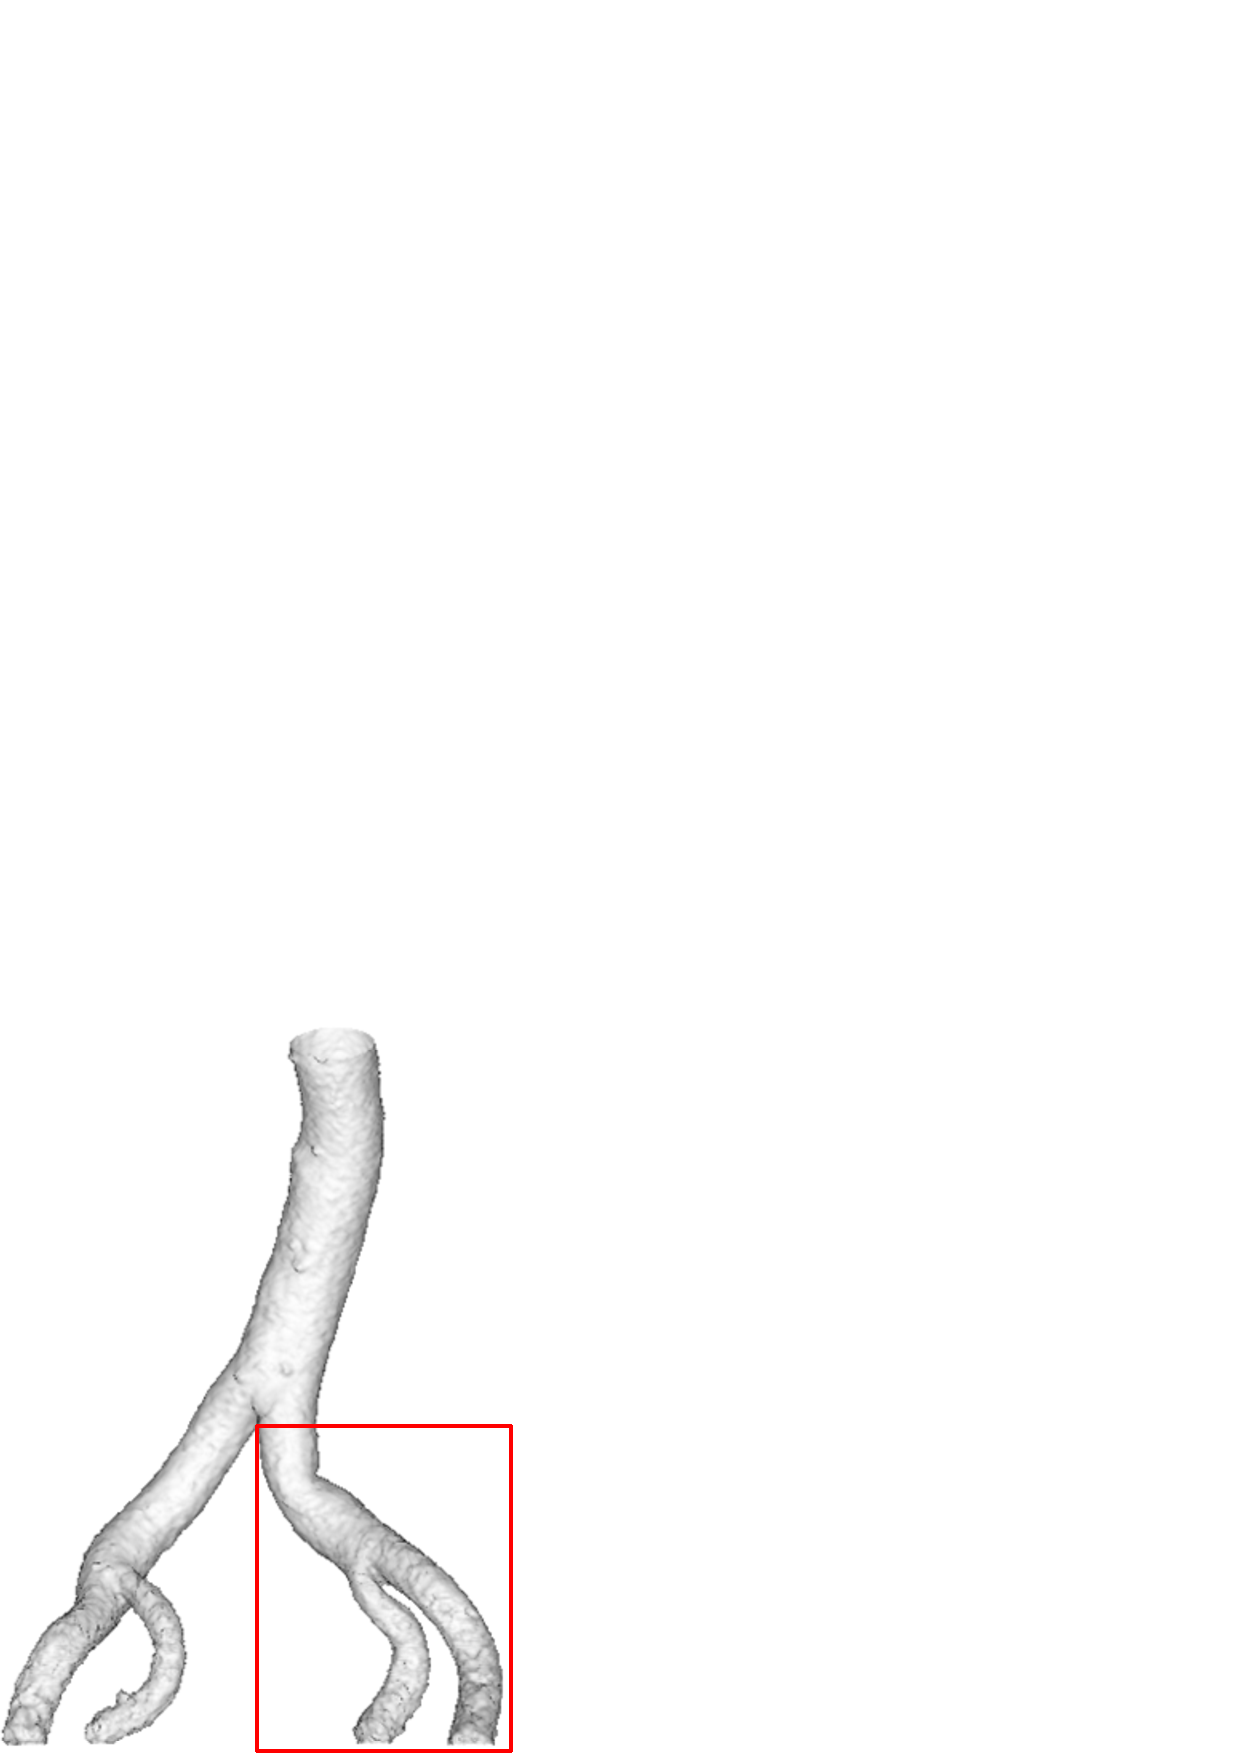
\includegraphics[height=2.4in]{Figures/chap05/VOI.png}
\caption{The original model surface (consists of $205,590$ polygons) and the VOI-extracted local part (in red square).}
\label{fig:VOI}
\end{figure}

%\subsection{Preprocessing for Centerline Extraction}

\subsection{Validating Connectivity of Image-Based Surface Model}

Before actually extracting the centerlines, the image-based surface model of the vasculature needs to be properly conditioned such that the computation can be operated successfully. %
The initial pass is the validation of the connectivity among the adjacent polygonal surfaces that consists of the whole visualization model.
The aim of this step is to find and connect the largest connected region in the given surface model (see Fig. \ref{fig:ConnectivityLocal}).
Table \ref{tbl:Connectivity} shows that the quantities of the consisting polygonal surfaces were not changed in local cases, whilst were decreased in global cases.
The former implies that the given (local) model was the largest connected region in the surface model before the validation.
The latter indicates that the largest connected region of the given model surface was fully extracted through the validation.
\begin{figure}[t]
\centering
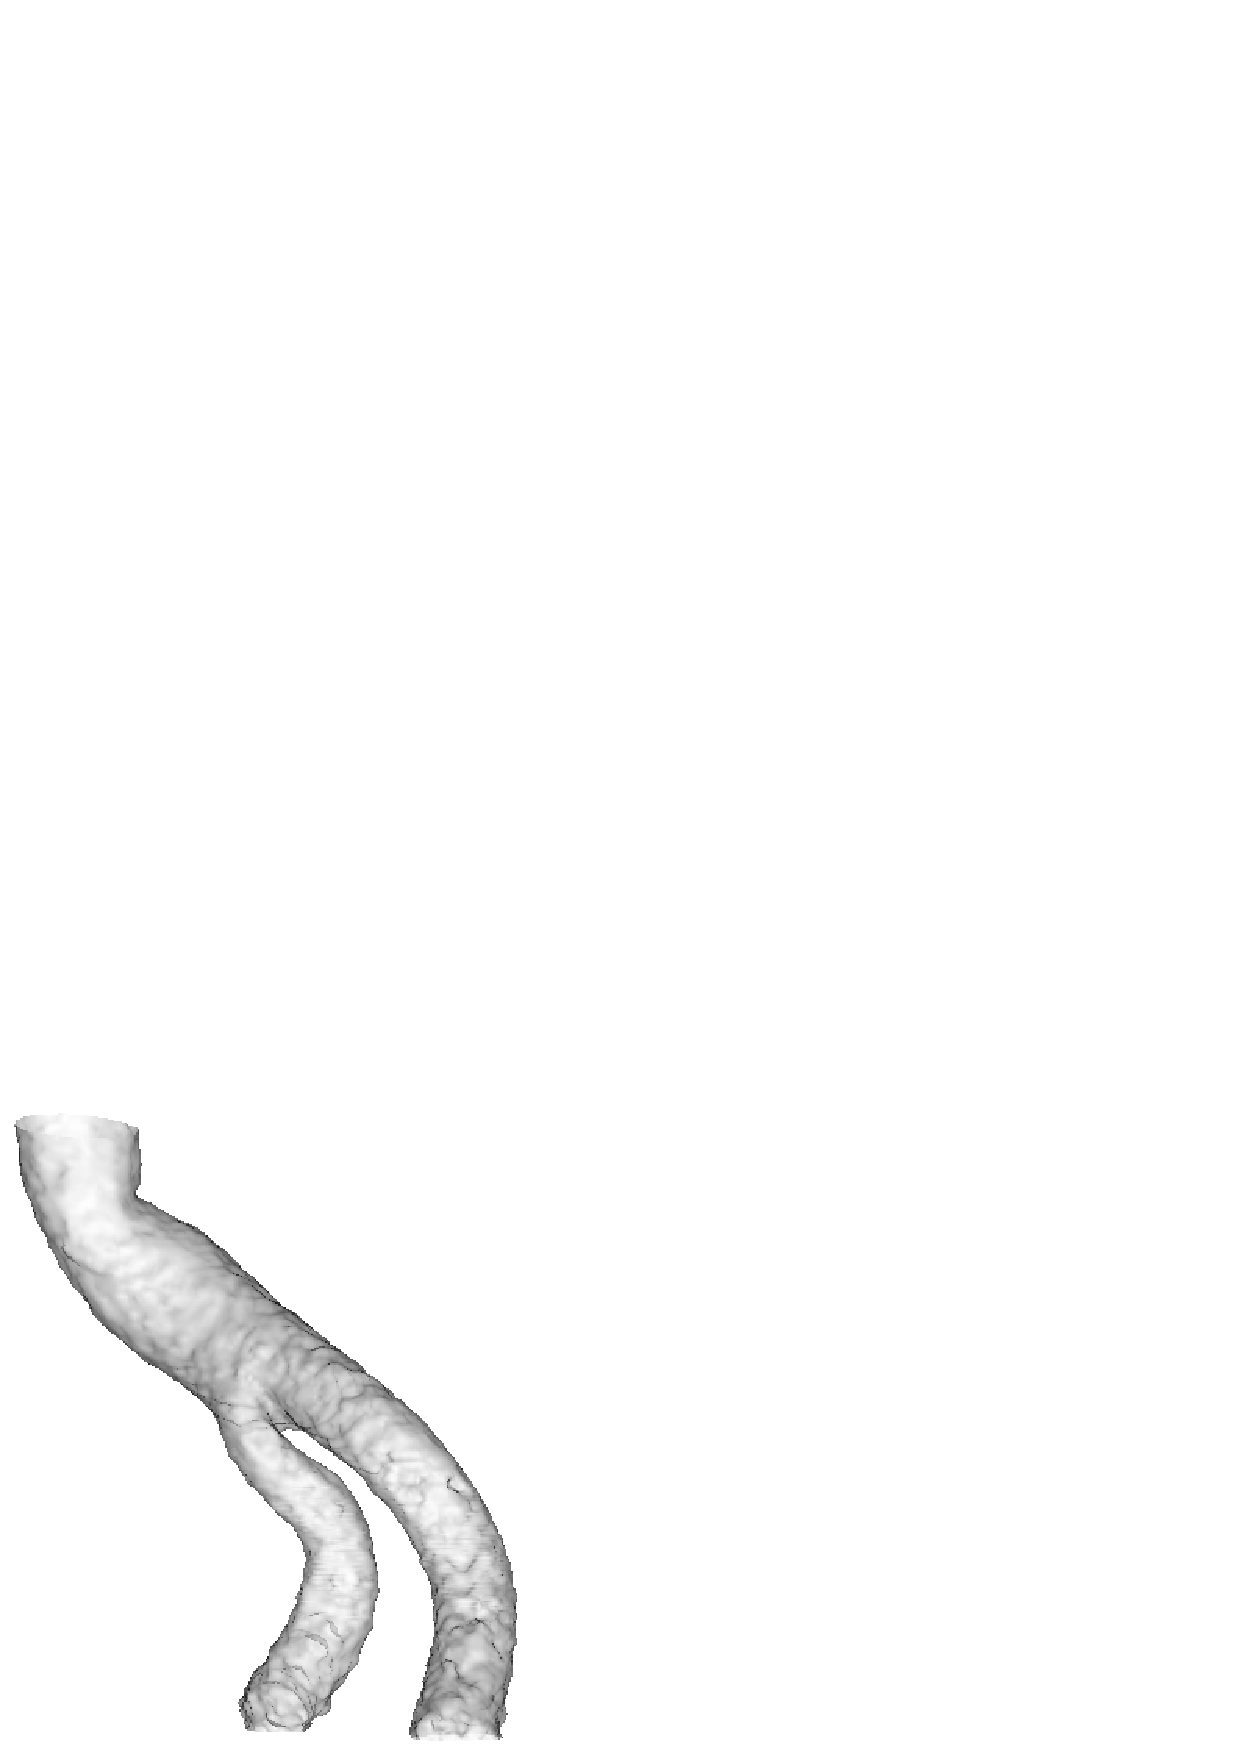
\includegraphics[width=1.5in]{Figures/chap05/connectivity_local.png}
\caption{Results of connectivity validation of model surface in local details (quantity of consisting polygons: $70,625$).}
\label{fig:ConnectivityLocal}
\end{figure}

\begin{table}[t]
\renewcommand{\arraystretch}{1.3}
\caption{Quantities of polygons before and after connectivity validation}
\label{tbl:Connectivity}
\centering
\begin{tabular}
{@{}llr@{}}
%{@{}llrr@{}}
\toprule
%\hline
%~      & ~                       & \multicolumn{2}{c}{Quantities} \\
%\cmidrule(4){3-4}
%~      & ~                       & Vertices & Polygons            \\
~      &                         & Quantities of polygons \\
%\midrule
\hline\hline
%Local  & Before validation       & N/A      & 70,625  \\
%~      & After validation        & N/A      & 70,625  \\
Local  & Before validation       & $70,625$  \\
~      & After validation        & $70,625$  \\
\hline\hline
%Global & Before validation       & N/A      & 205,590 \\
%~      & After validation        & N/A      & 205,452 \\
Global & Before validation       & $205,590$ \\
~      & After validation        & $205,452$ \\
\bottomrule
%\hline
\end{tabular}
\end{table}
\begin{figure}[t]
\centering
\subfloat{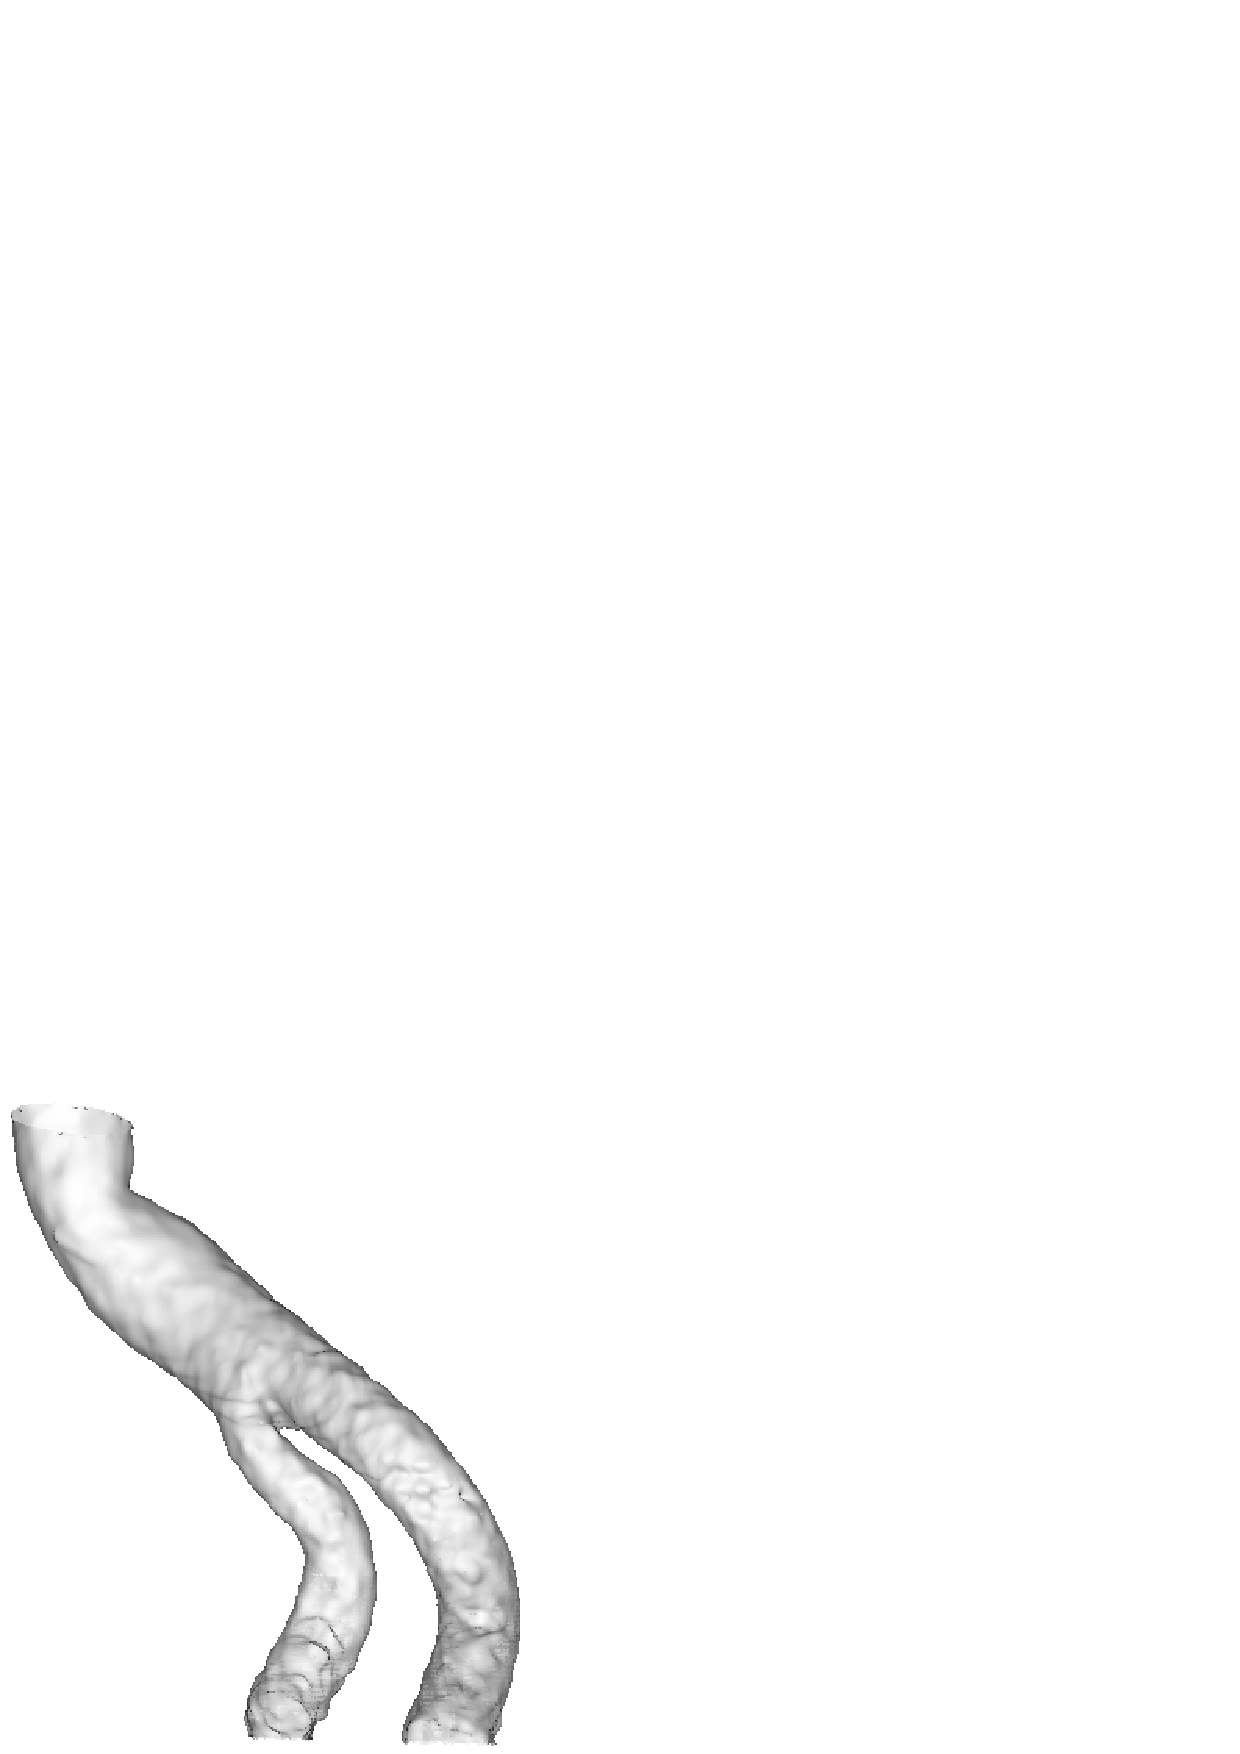
\includegraphics[width=1.5in]{Figures/chap05/smooth_30_1_local.png}%
\label{fig:Smooth30-1Local}}
\hfil
\subfloat{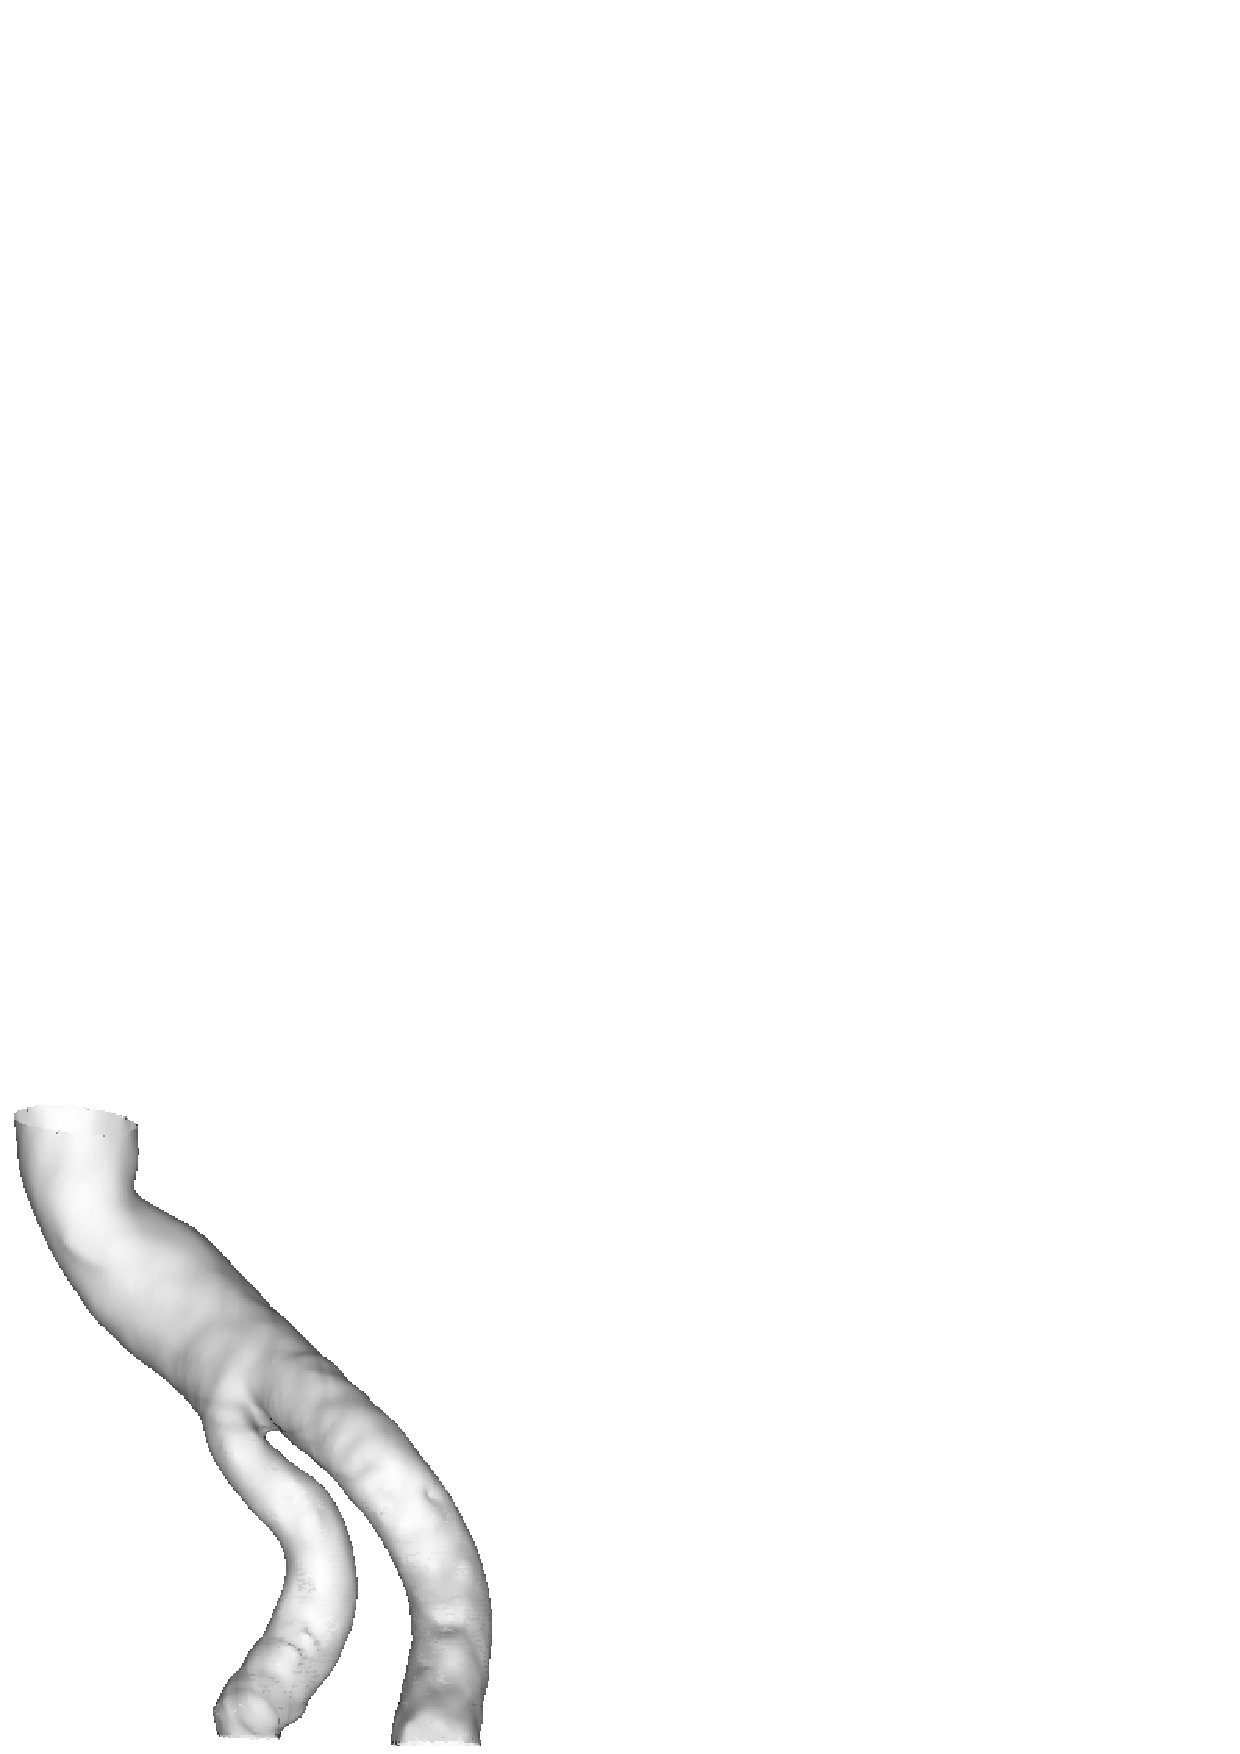
\includegraphics[width=1.45in]{Figures/chap05/smooth_30_01_local.png}%
\label{fig:Smooth30-01Local}}
\hfil
\subfloat{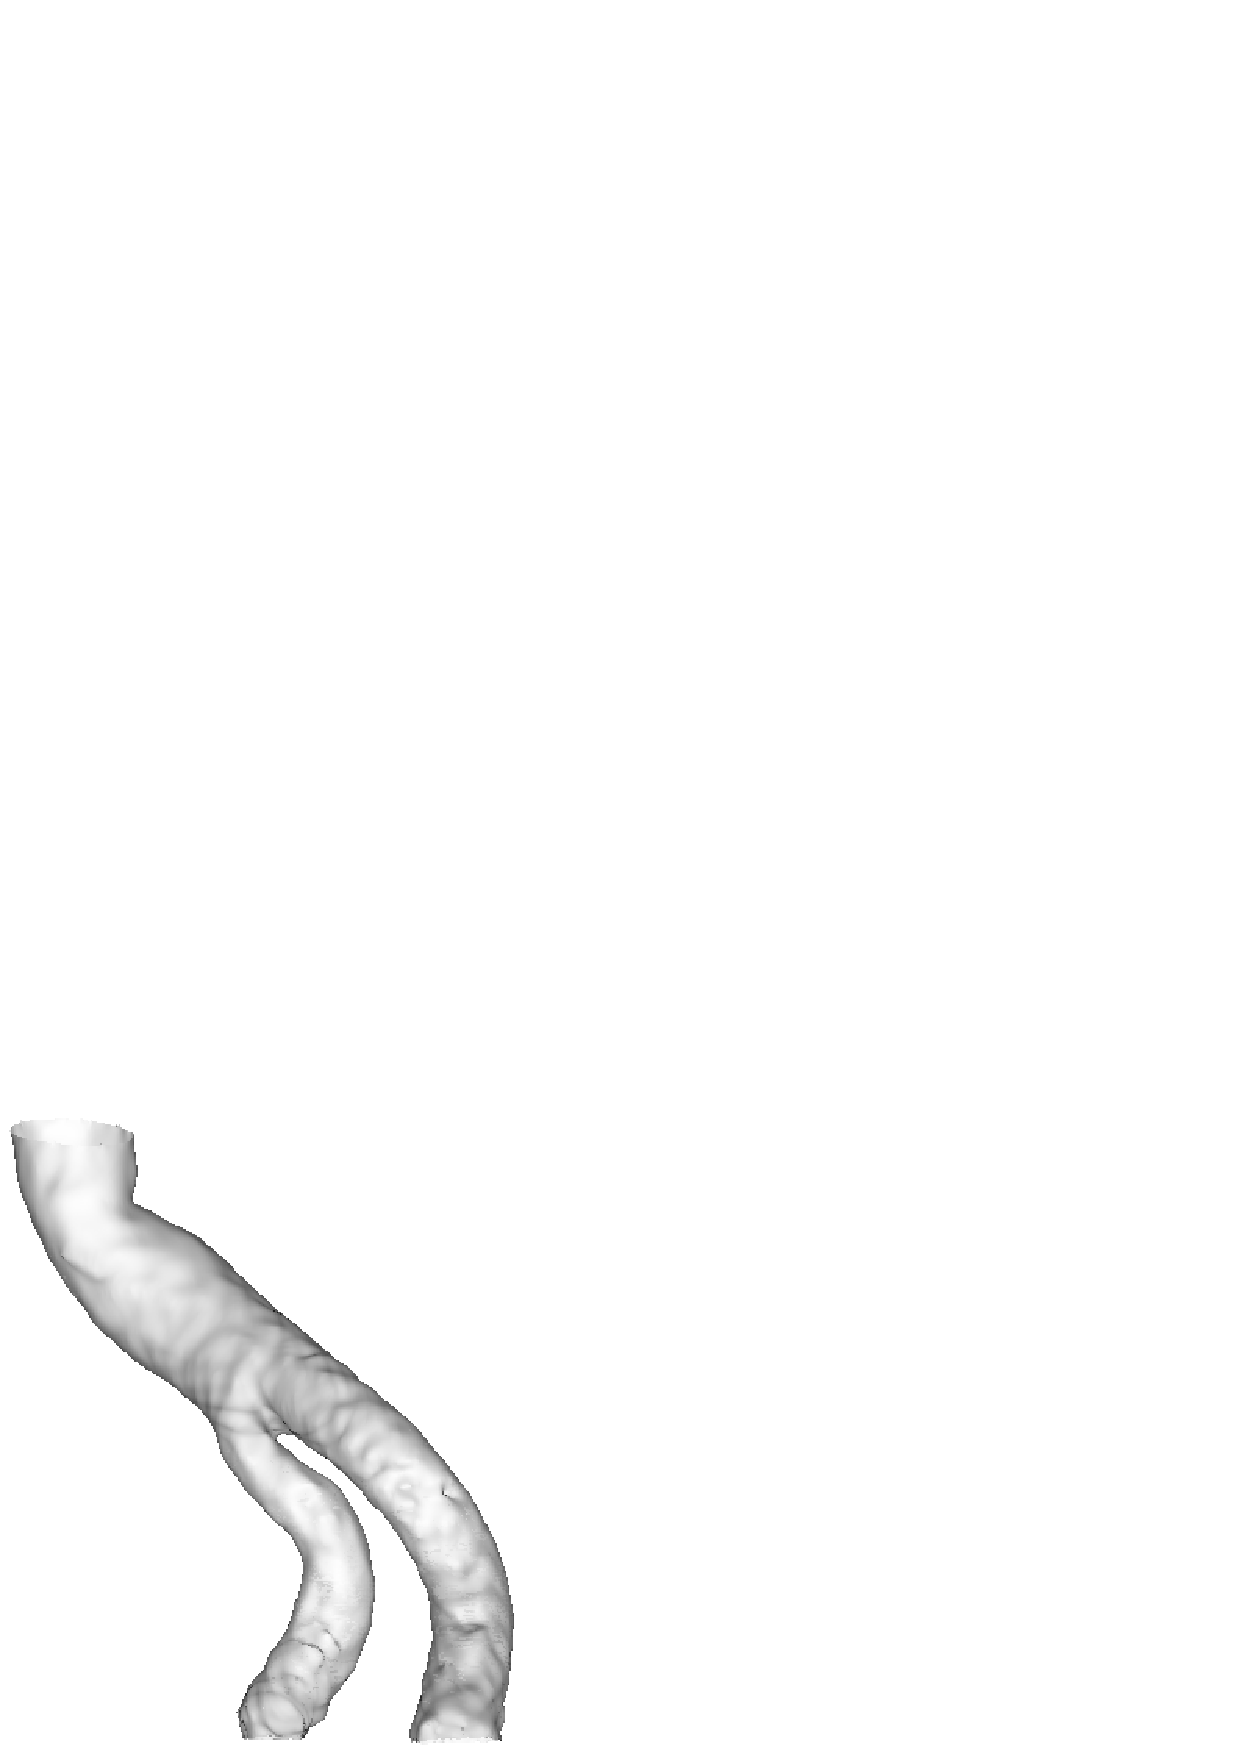
\includegraphics[width=1.5in]{Figures/chap05/smooth_100_1_local.png}%
\label{fig:Smooth100-1Local}}
\hfil
\subfloat{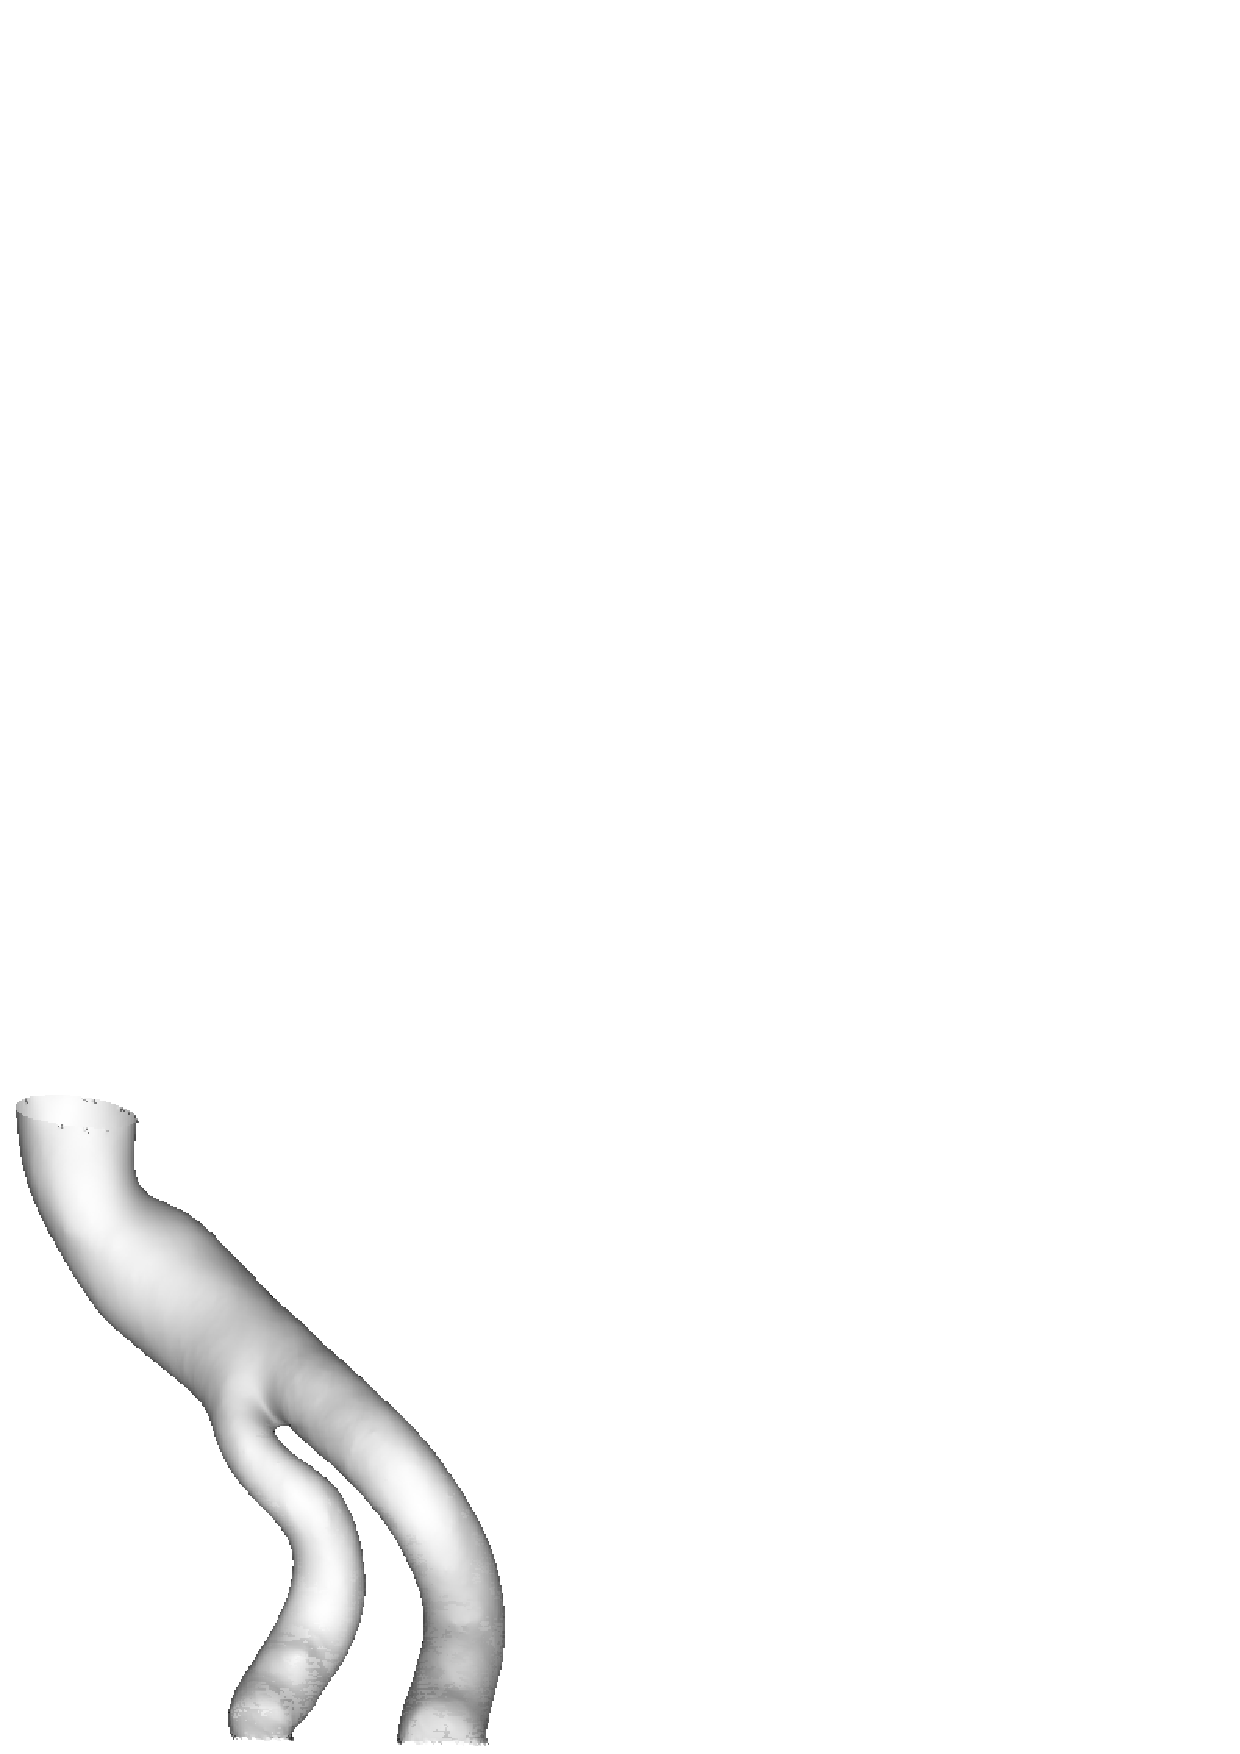
\includegraphics[width=1.45in]{Figures/chap05/smooth_100_01_local.png}%
\label{fig:Smooth100-01Local}}
\caption{Smoothing effects by applying different parameters: (a) $\text{pass band} = 0.1$, $\text{iterations} = 30$; (b) $\text{pass band} = 0.01$, $\text{iterations} = 30$; (c) $\text{pass band} = 0.1$, $\text{iterations} = 100$; (d) $\text{pass band} = 0.01$, $\text{iterations} = 100$.}%
\label{fig:SmoothLocal}
\end{figure}

%\begin{table}
%\renewcommand{\arraystretch}{1.3}
%\caption{Comparison of quantities of polygonal surfaces - Part I}
%\label{tbl:Eigenvalues}
%\centering
%\begin{tabular}{l||r}
%\hline
%\bfseries Connectivity validation & \bfseries Quantities \\
%\hline\hline
%Before                            & 757,538 \\
%After                             & 757,400 \\
%\hline
%\end{tabular}
%\end{table}

\subsection{Smoothing Connected Surface Model}

The centerline extracting method adopted in this work is sensitive to the noises on the input surface.
Due to the poor quality in some level of details of the original images, segmentation may introduce unnecessary uneven surfaces.
These artifacts in the surfaces can cause difficulties in the delivering of the virtual guidewires towards the hesion along the lumen of the model vessels.
To depress the noisy surface of the model, a surface smoothing module implemented based on low-pass filtering is applied.
There are two parameters associated with the smoothing module.
One of them specifies the number of iterations, which is equivalent to the degree of the polynomial approximating the windowed sinc function defined by (\ref{eqn:Approximation}).
The other determines the pass band of this low-pass filtering module.
Different sets of parameters were fed to the smoothing module in order to find the best results for the following processing (see Fig. \ref{fig:SmoothLocal}).
Observing these results, the parameters ($\text{pass band} = 0.01$, $\text{iterations} = 100$) used to generating the resulting surface in Fig. \ref{fig:Smooth100-01Local} demonstrated better effects than the rest.
%\begin{figure}[t]
%\centering
%\subfloat[]{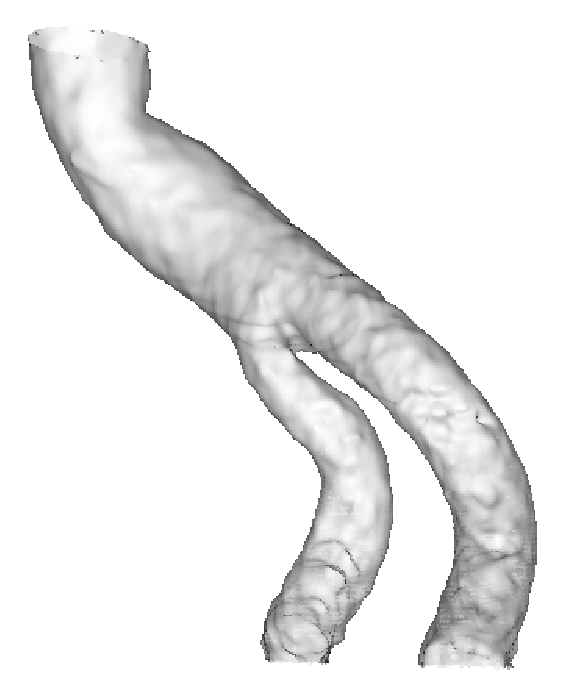
\includegraphics[width=1.5in]{../Figures/smooth_30_1_local.eps}%
%\label{fig:Smooth30-1Local}}
%\hfil
%\subfloat[]{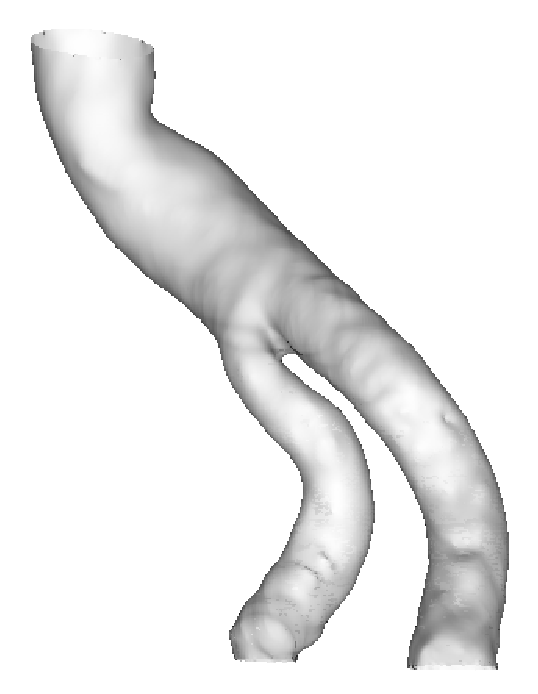
\includegraphics[width=1.45in]{../Figures/smooth_30_01_local.eps}%
%\label{fig:Smooth30-01Local}}
%\hfil
%\subfloat[]{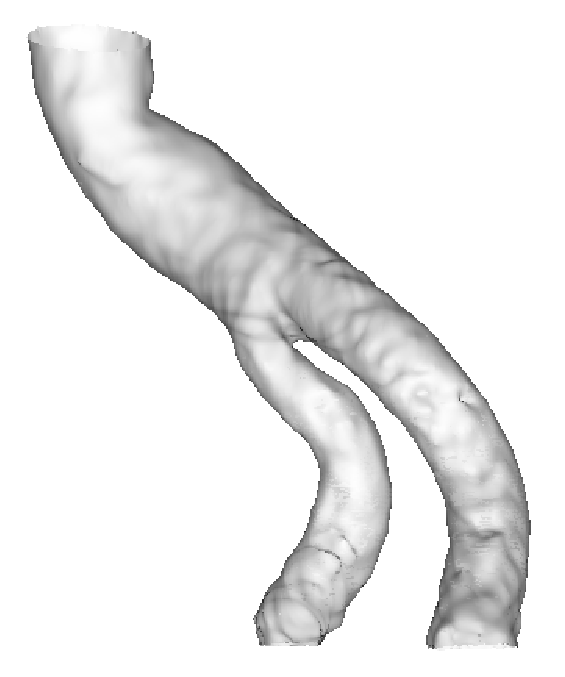
\includegraphics[width=1.5in]{../Figures/smooth_100_1_local.eps}%
%\label{fig:Smooth100-1Local}}
%\hfil
%\subfloat[]{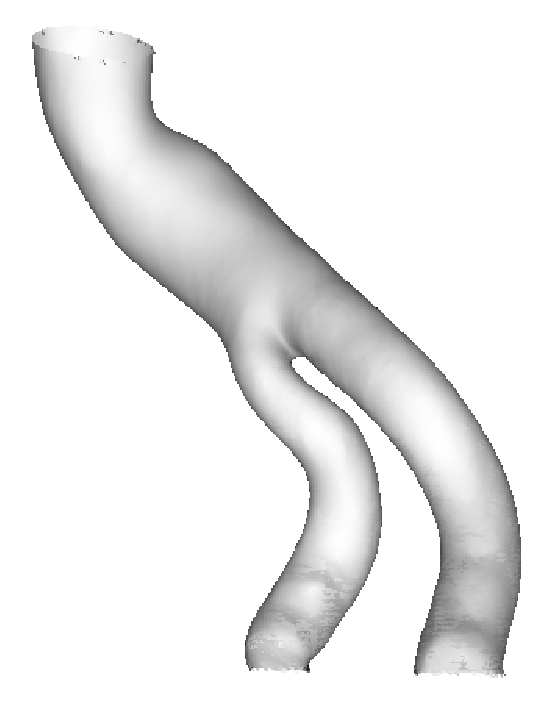
\includegraphics[width=1.45in]{../Figures/smooth_100_01_local.eps}%
%\label{fig:Smooth100-01Local}}
%\caption{Smoothing effects by applying different parameters: (a) $\text{pass band} = 0.1$, $\text{iterations} = 30$; (b) $\text{pass band} = 0.01$, $\text{iterations} = 30$; (c) $\text{pass band} = 0.1$, $\text{iterations} = 100$; (d) $\text{pass band} = 0.01$, $\text{iterations} = 100$.}%
%\label{fig:SmoothLocal}
%\end{figure}

\subsection{Subdivision Using Improved Butterfly Scheme}

To further attenuate the effects of noisy surfaces on extraction of centerlines and increase the precision of the centerlines extraction, the number of the polygons consisting the model surface has to be increased.
In order to achieve this, the smoothed surface need to be subdivided without introducing more perturbation.
Figure \ref{fig:SubdivisionLocal} illustrates that the subdivision computation based on the improved butterfly scheme.
At the same time, the quantities of the consisting polygonal surfaces increased substantially after the subdivision complete (see Table \ref{tbl:Subdivision}).
Comparing the quantities of the polygons before and after the subdivision in both cases, the quantities of the resulting polygons are about four times greater than the quantities of the input polygons due to the subdivision scheme employed in this work.
\begin{figure}[t]
\centering
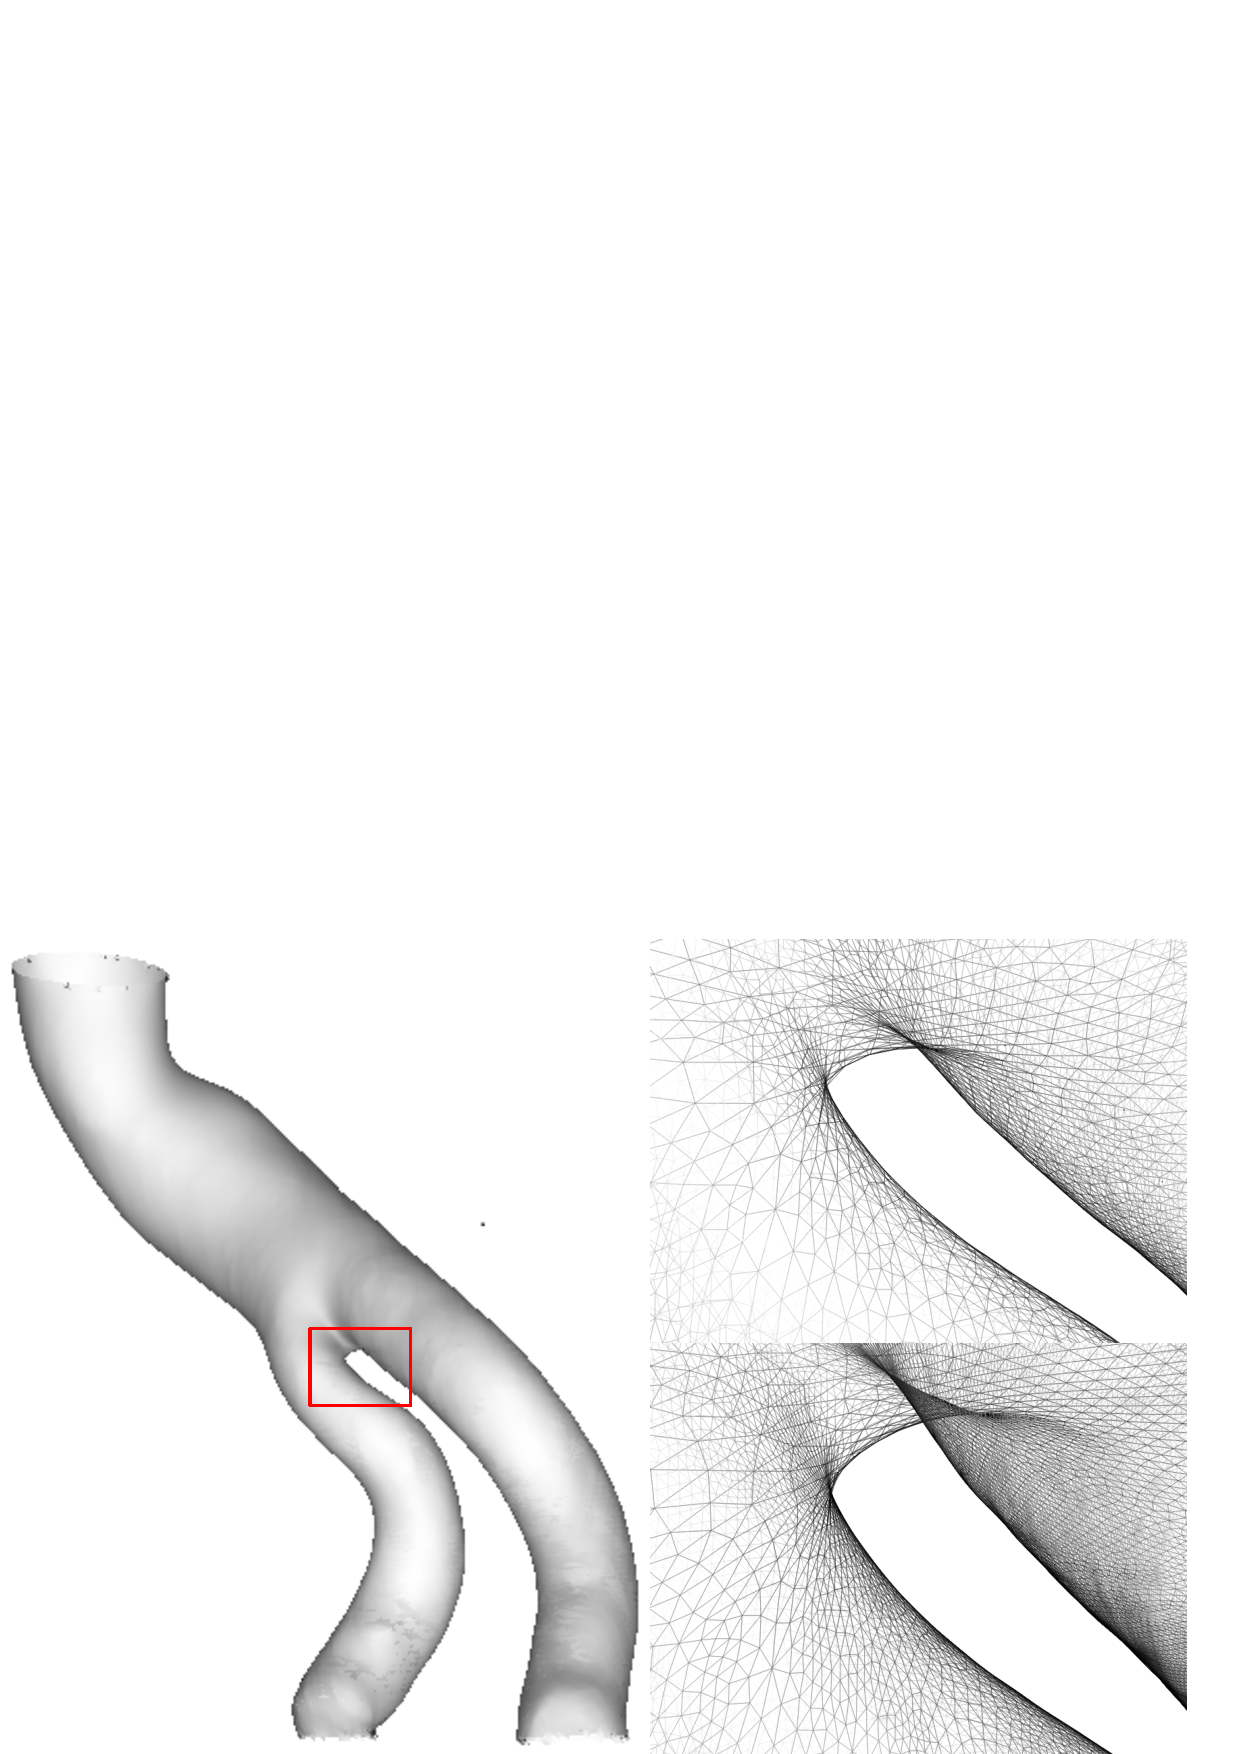
\includegraphics[width=3.0in]{Figures/chap05/subdivision.png}
\caption{Subdivision of smoothed surface by using improved butterfly scheme. \emph{Left}: subdivision in local details. \emph{Top right}: polyhedral surface before subdivision. \emph{Bottom right}: polyhedral surface after subdivision.}%
\label{fig:SubdivisionLocal}
\end{figure}

\begin{table}[t]
\renewcommand{\arraystretch}{1.3}
\caption{Quantities of polygons before and after subdivision using an improved butterfly scheme}
\label{tbl:Subdivision}
\centering
\begin{tabular}
%{@{}llr@{}}
{@{}llrr@{}}
\toprule
%\hline
%~      & ~                       & \multicolumn{2}{c}{Quantities} \\
%\cmidrule(4){3-4}
%~      & ~                       & Vertices & Polygons            \\
~      &                         & Quantities of polygons & Percentages ($\%$)\\
%\midrule
\hline\hline
%Local  & Before subdivision      & N/A      &  70,625  \\
%~      & After subdivision       & N/A      & 281,060  \\
Local  & Before subdivision      &  $70,625$  &\\
~      & After subdivision       & $281,060$  & 398 \\
\hline\hline
%Global & Before validation       & N/A      & 205,452  \\
%~      & After validation        & N/A      & 821,808  \\
Global & Before validation       & $205,452$  &\\
~      & After validation        & $821,808$  & 400 \\
\bottomrule
%\hline
\end{tabular}
\end{table}

%\begin{table}
%\renewcommand{\arraystretch}{1.3}
%\caption{Comparison of quantities of polygonal surfaces - Part II}
%\label{tbl:Eigenvalues}
%\centering
%\begin{tabular}{l||r}
%\hline
%\bfseries Subdivision  & \bfseries Quantities \\
%\hline\hline
%Before                 &  757,400 \\
%After                  & 3,029,600 \\
%\hline
%\end{tabular}
%\end{table}

\begin{figure}[t]
\centering
\subfloat{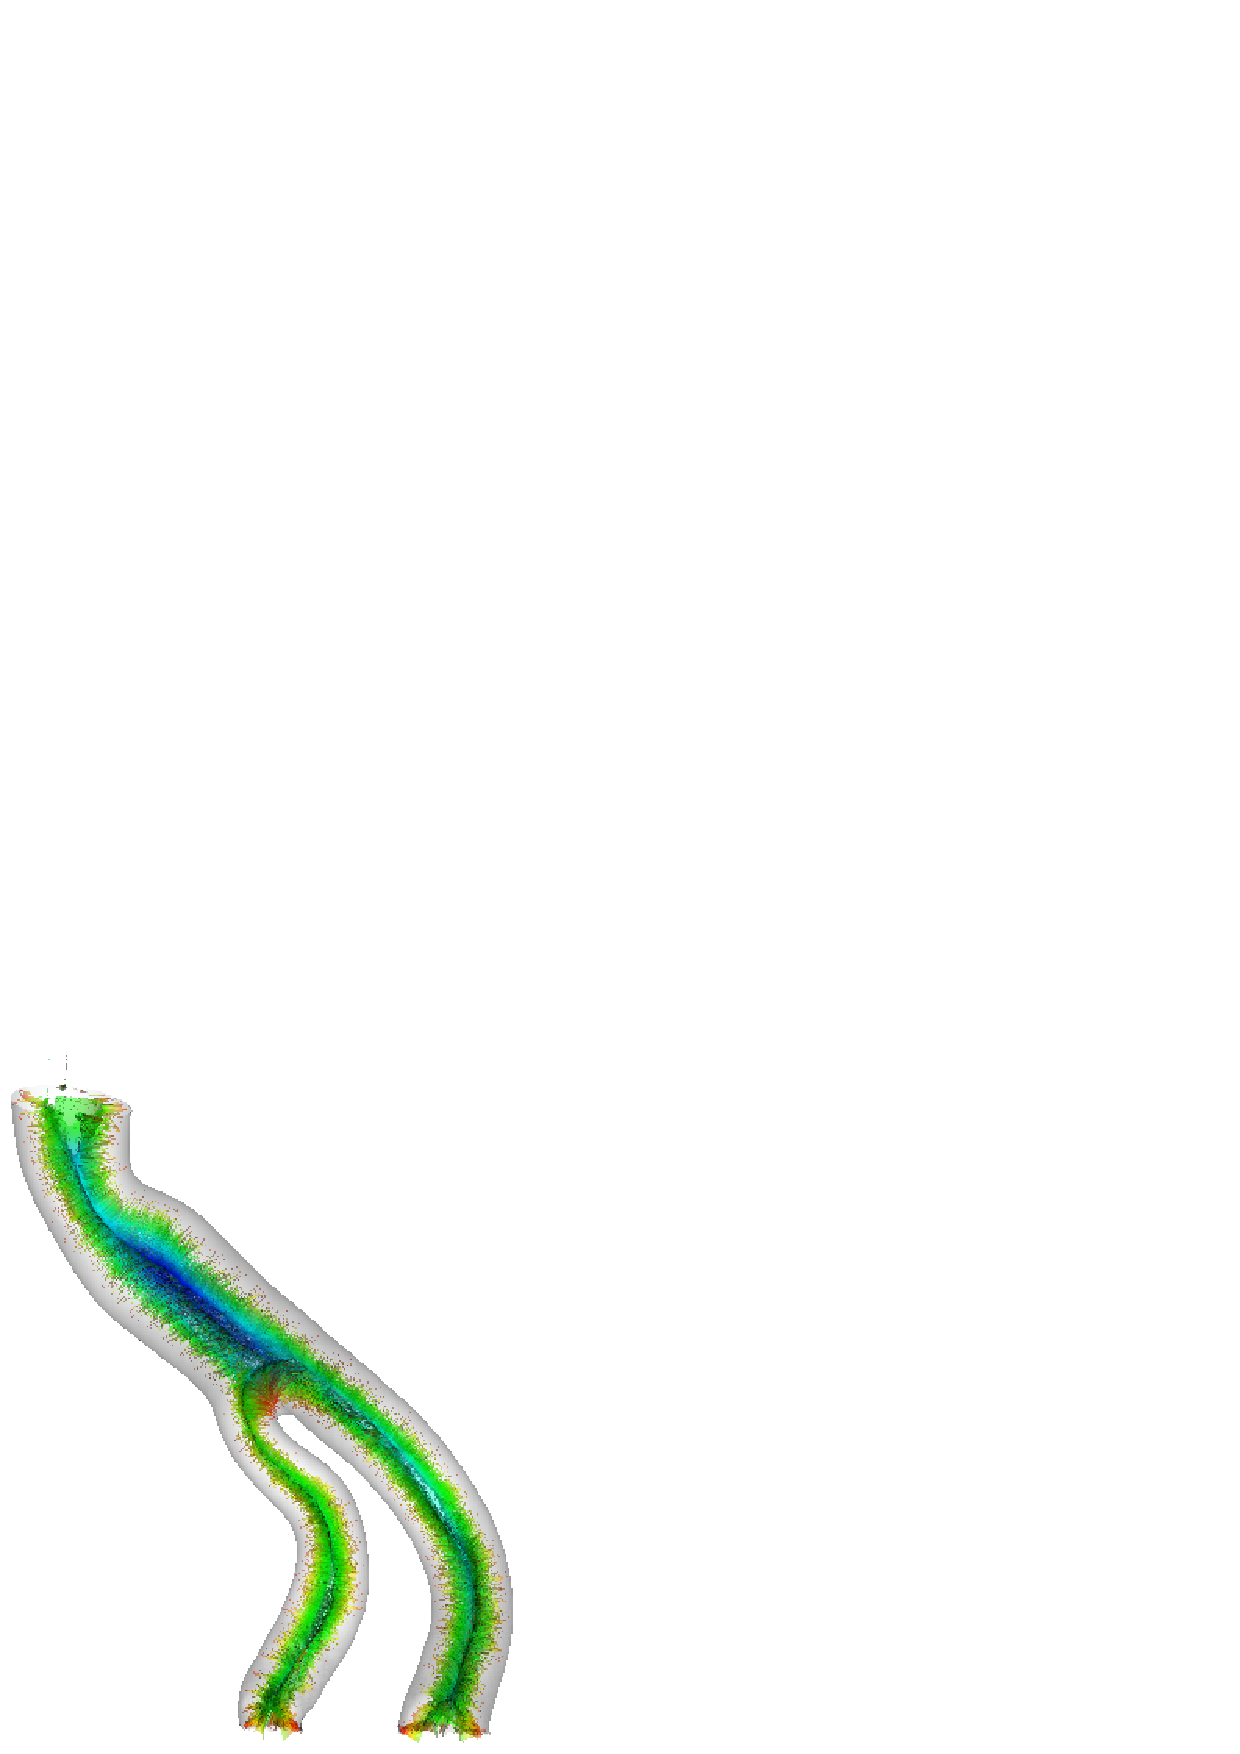
\includegraphics[width=1.5in]{Figures/chap05/overlay_100_01_voronoi_local.png}%
\label{fig:VoronoiLocal}}
\hfil
\subfloat{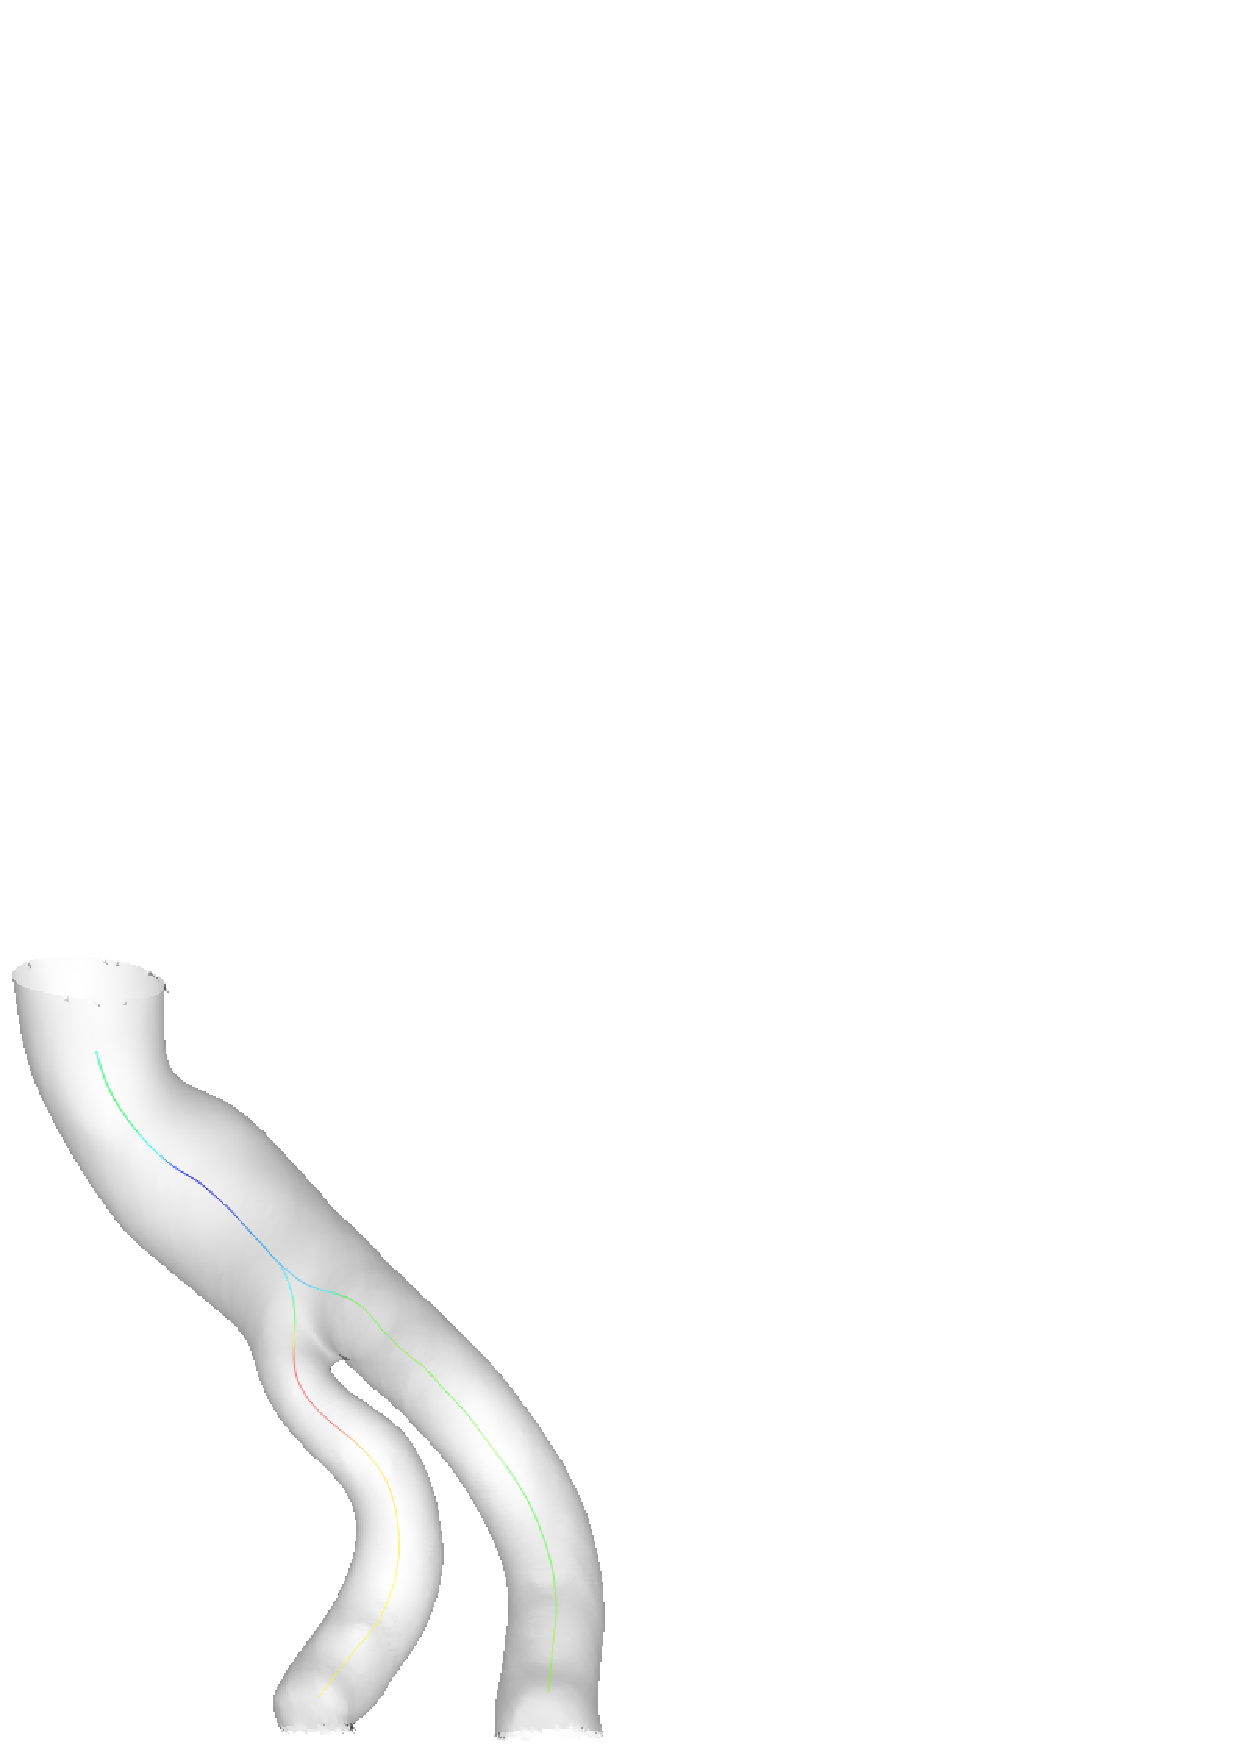
\includegraphics[width=1.5in]{Figures/chap05/overlay_100_01_centerlines_local.png}%
\label{fig:OverlayLocal}}
\caption{Centerlines extraction of the aorta in local details: (a) embedded Voronoi diagram; (b) centerlines inside the vessel.}%
\label{fig:CenterlinesLocal}
\end{figure}

\begin{figure}[t]
\centering
\subfloat{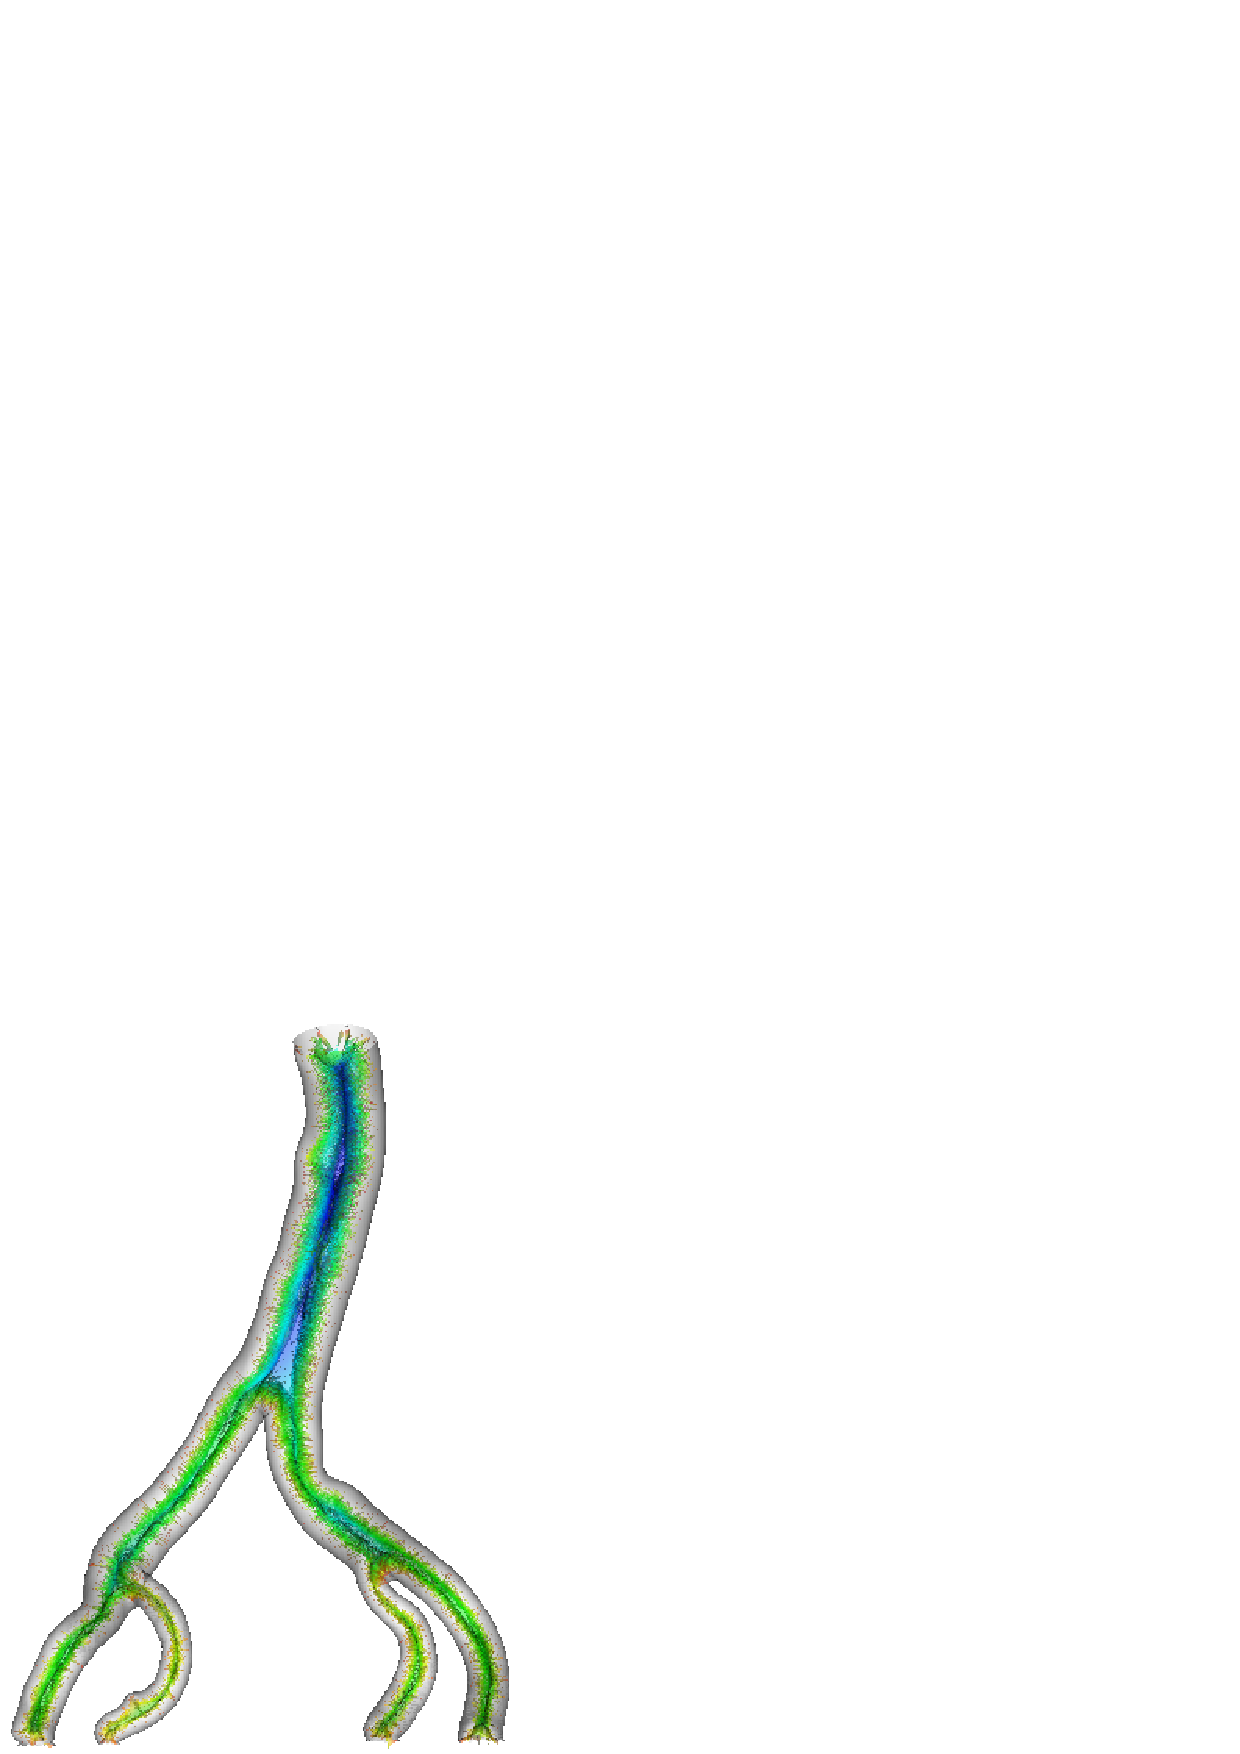
\includegraphics[height=2.0in]{Figures/chap05/overlay_100_01_voronoi.png}
%\caption{Voronoi diagrams of the abdominal aorta.}
\label{fig:VoronoiGlobal}}
\hfil
\subfloat{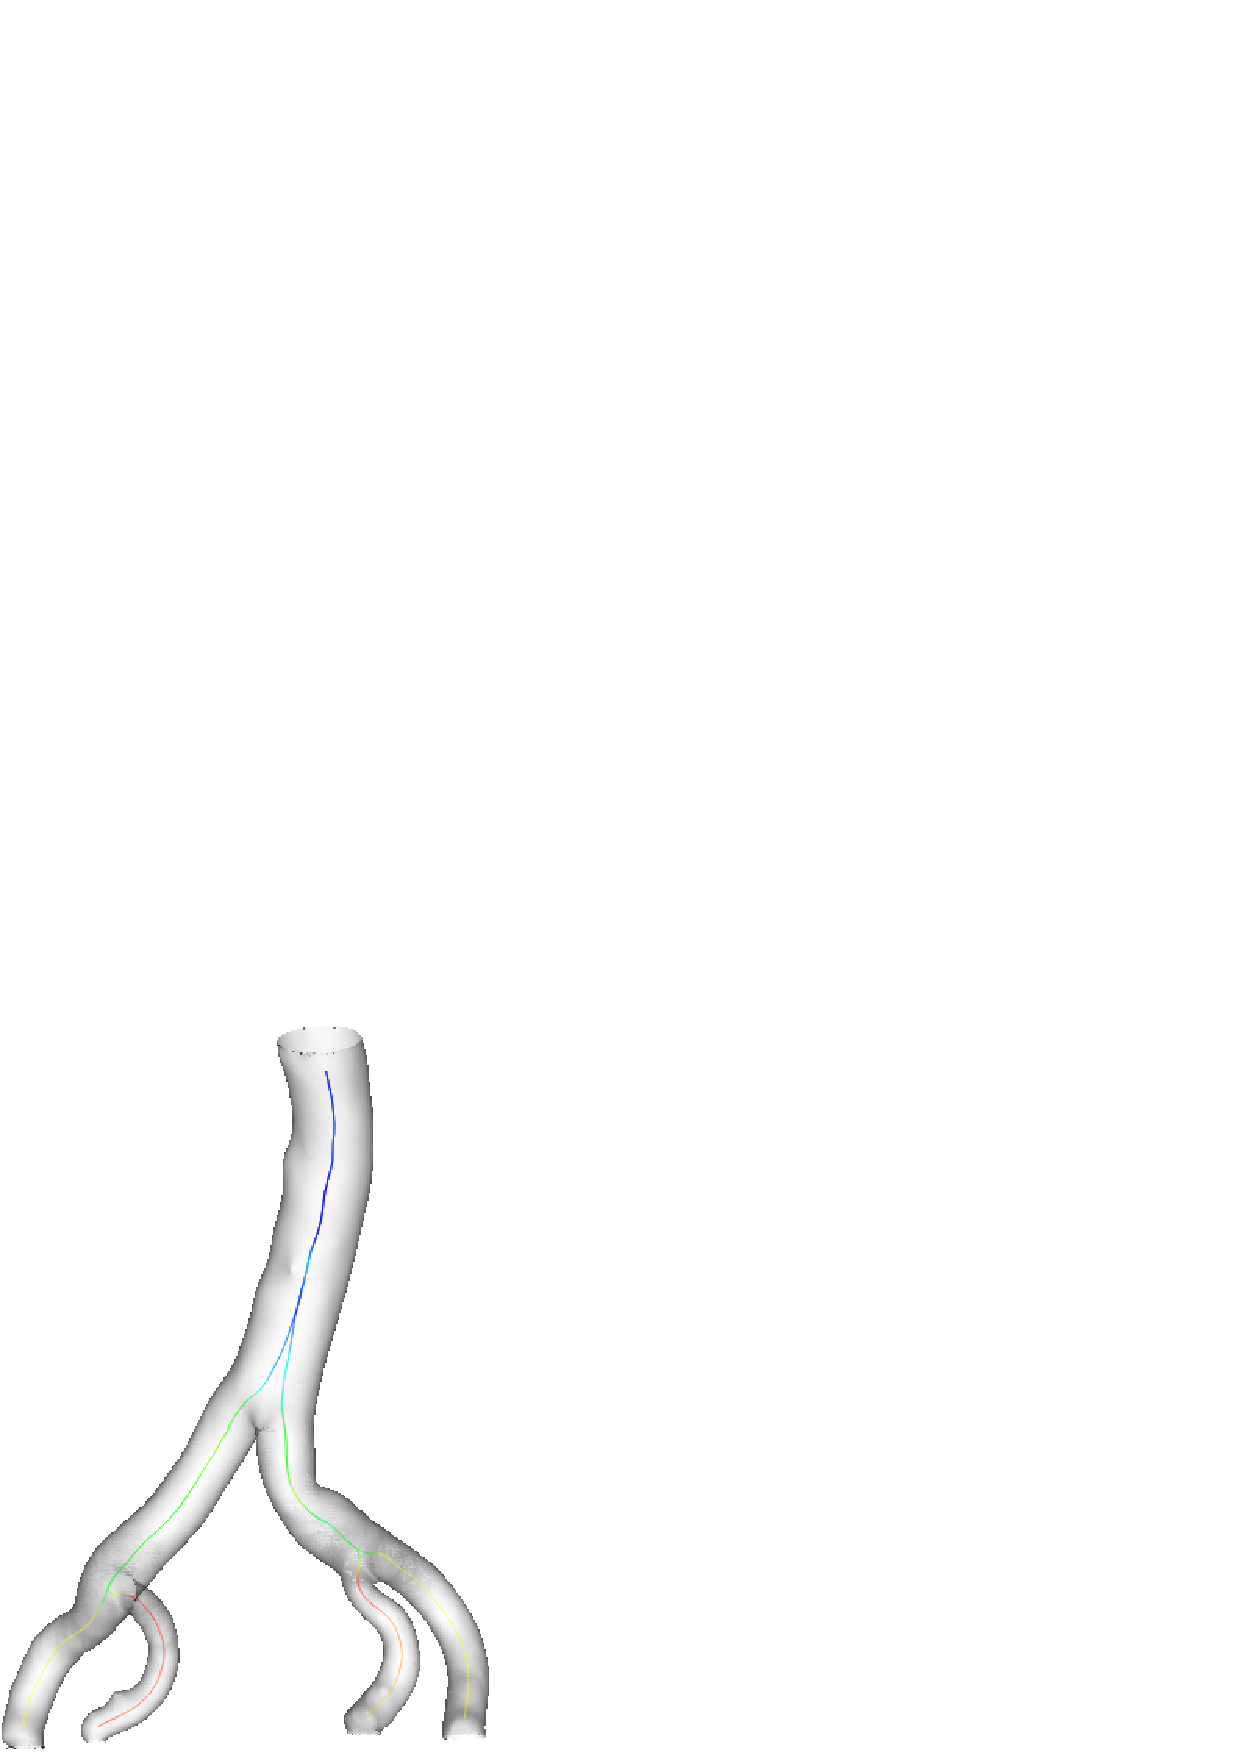
\includegraphics[height=2.0in]{Figures/chap05/overlay_100_01_centerlines.png}
%\caption{Centerlines of the abdominal aorta.}
\label{fig:OverlayGlobal}}
\caption{Centerlines extraction of the aorta in VOI. (a) Voronoi diagrams; (b) Centerlines. }
\label{fig:CenterlineGlobal}
\end{figure}

\subsection{Centerlines Extraction Based on Surface Model}

The centerlines extraction computation was performed on the subdivided surface model.
Firstly, the embedded Voronoi diagram of the preprocessed surface model is generated (see Fig. \ref{fig:VoronoiLocal}).
Secondly, the centerlines of the tubular surface model is computed (see Fig. \ref{fig:OverlayLocal}).
The colors marked on the Voronoi diagram and the centerlines denote the diameters of the local resection circle, decreasing from blue to red.
The same processing was straightly applied to the model surface of the whole abdominal aorta (see Fig. \ref{fig:VoronoiGlobal} and Fig. \ref{fig:OverlayGlobal}).
One can see from the details of the results that the starting and ending points are not exactly located at the ``entrances" or ``exits".
The reason of this is the Voronoi diagram on which the points consisting the centerlines exist never intersect with the model surface, i.e., the ending points of the centerlines are approaching the terminals of the surface model as near as possible, but never stick to them.
\begin{figure}[t]
\centering
\subfloat{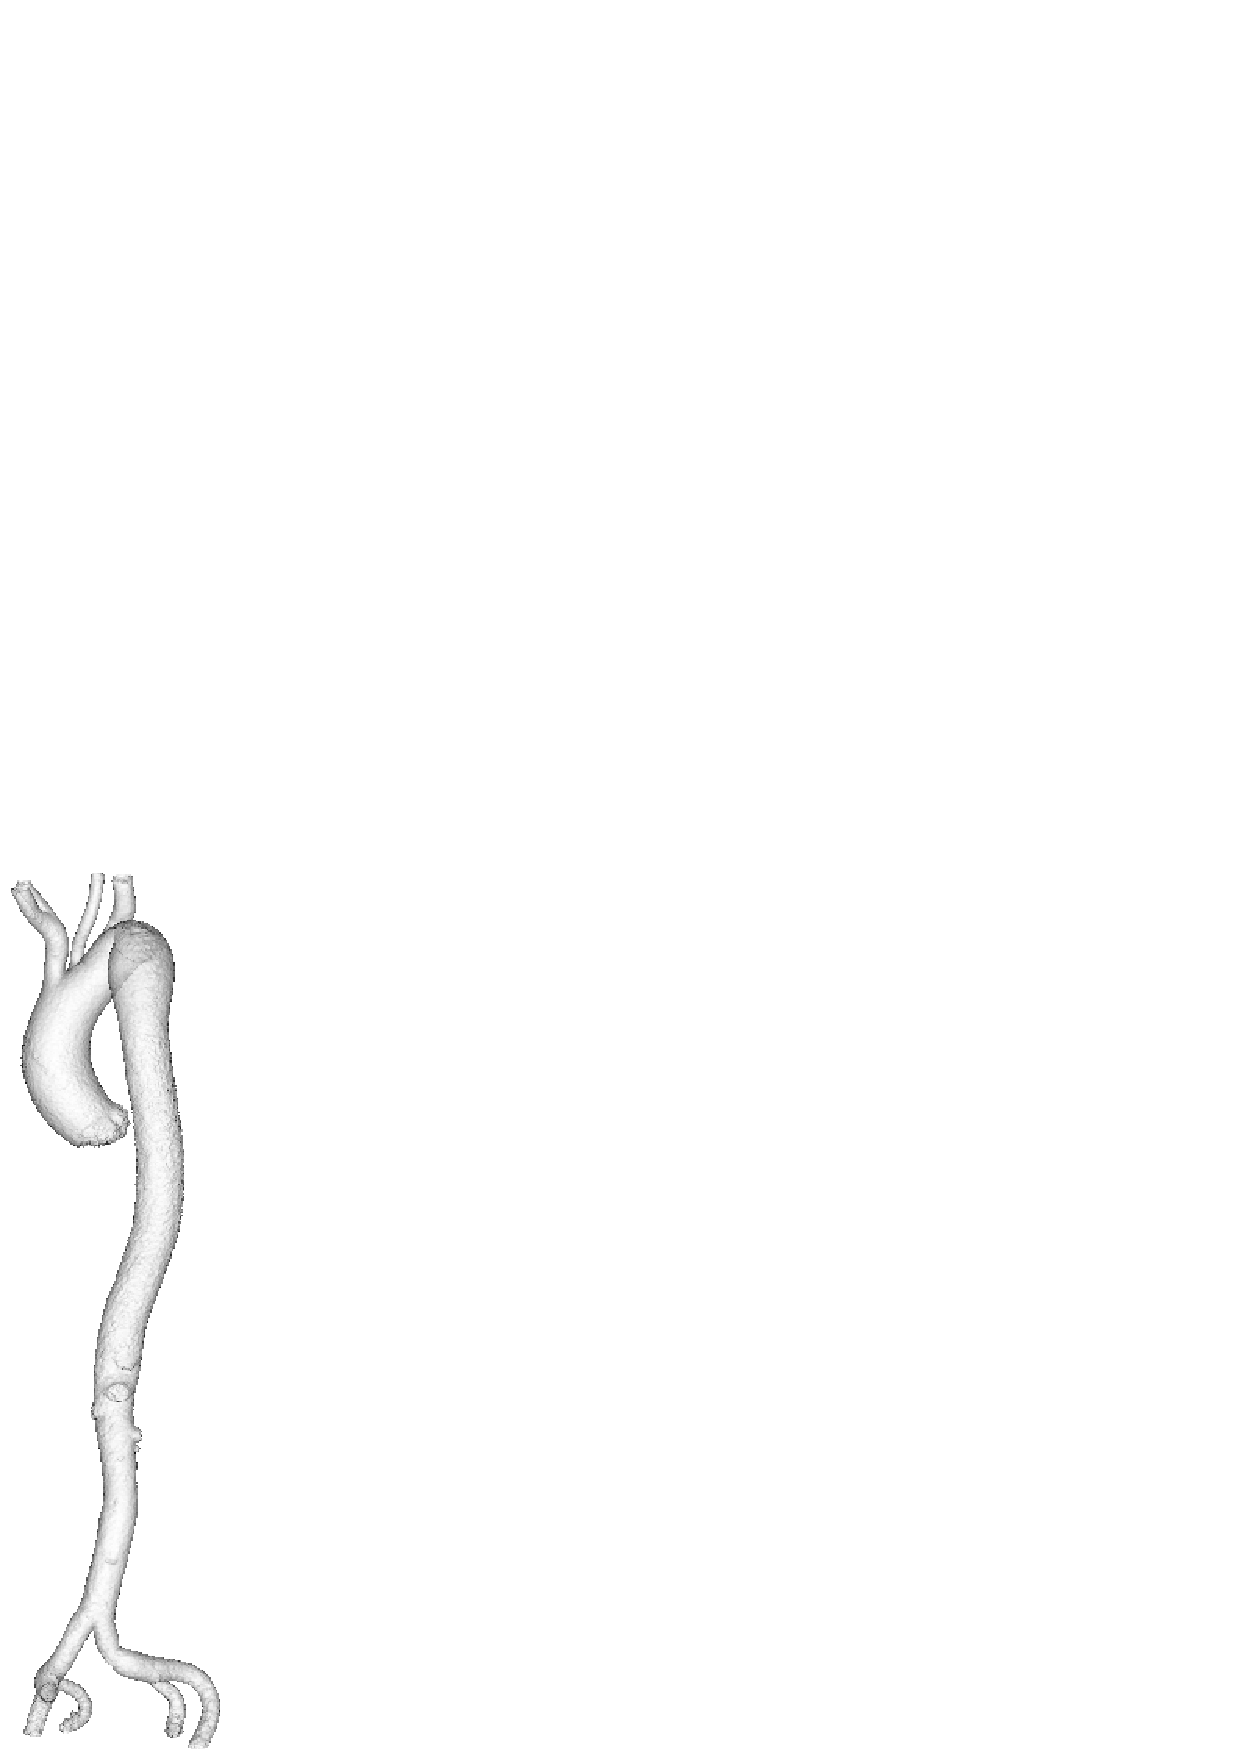
\includegraphics[width=0.7in]{Figures/chap05/surface.png}%
\label{fig:SurfaceModel}}
\hfil
\subfloat{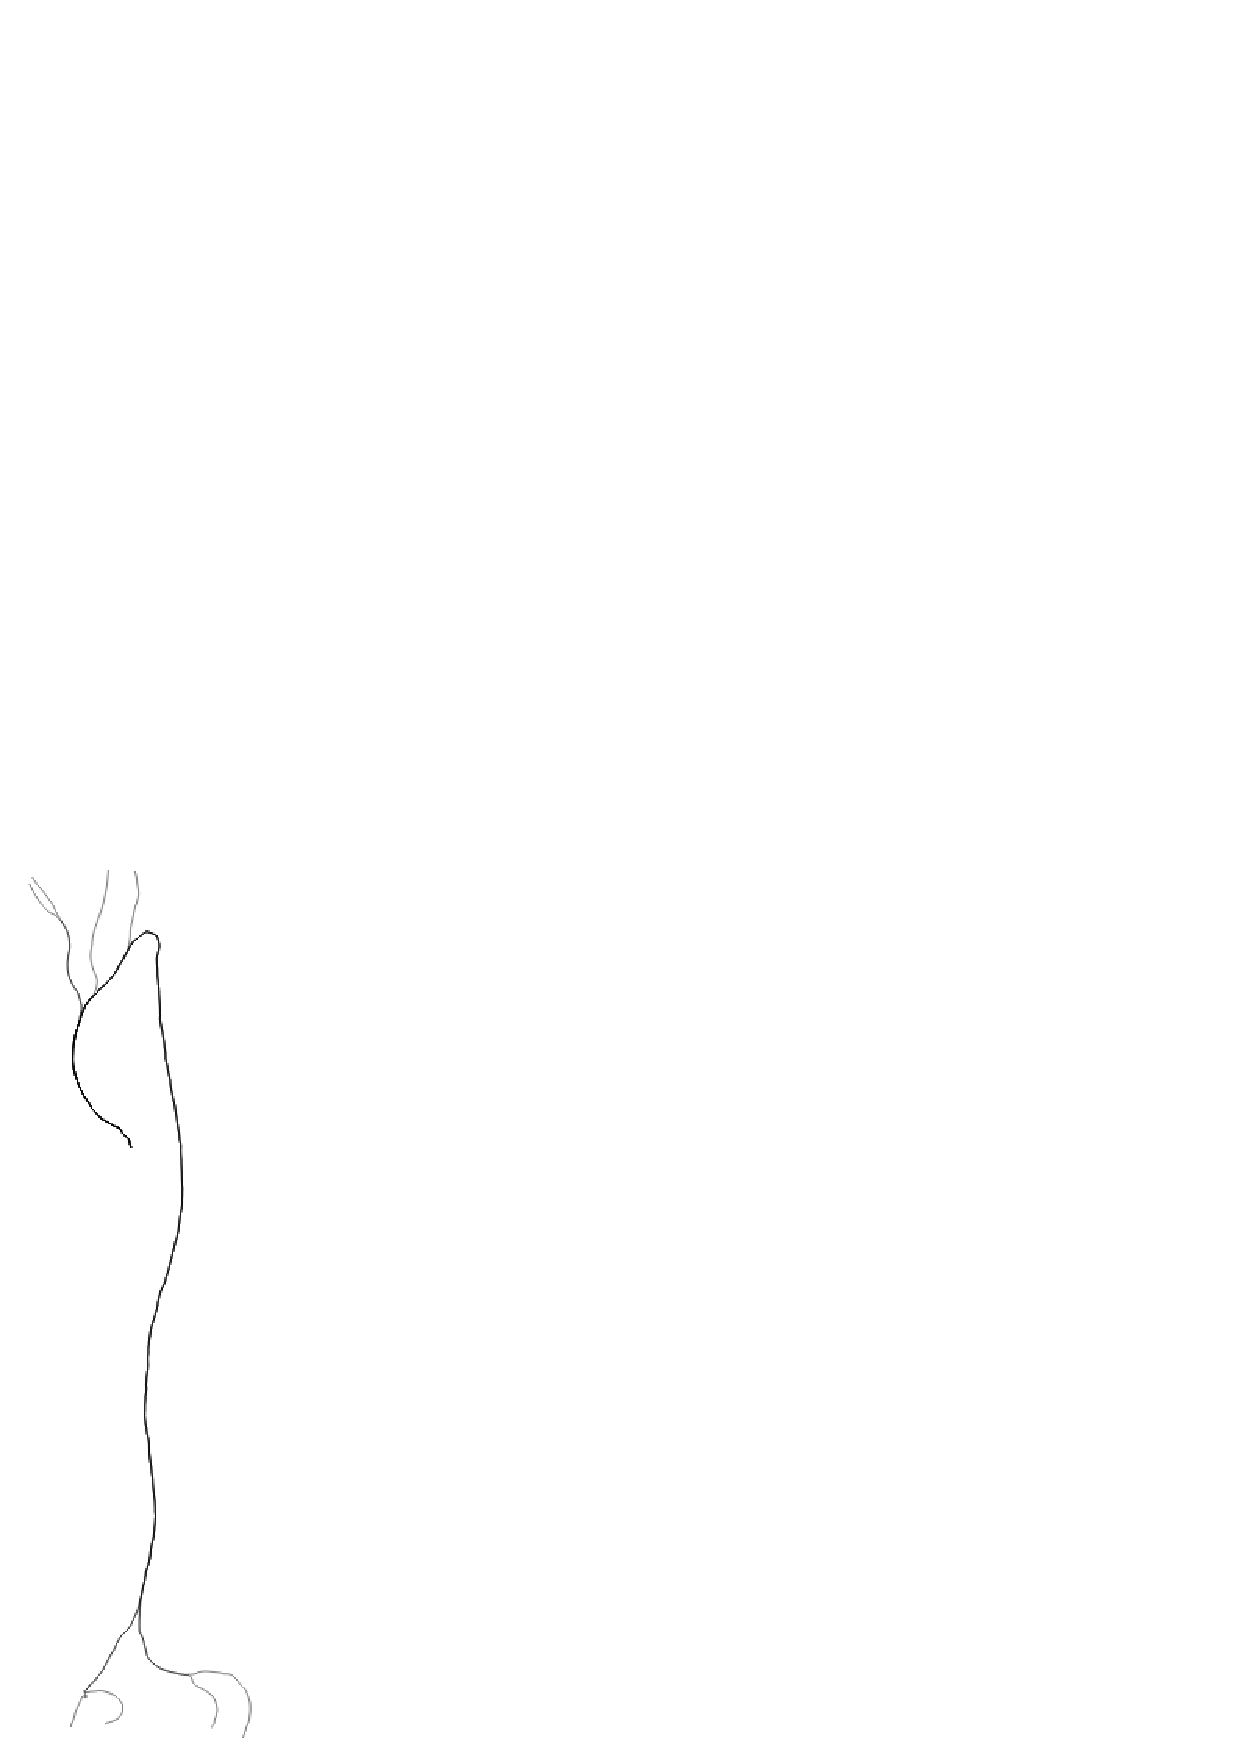
\includegraphics[width=0.9in]{Figures/chap05/centerlines.png}%
\label{fig:CenterlinesModel}}
\caption{Visualization models of the aorta: (a) image-based surface model (quantity of consisting polygons: $757,538$); (b) centerlines of the surface model.}%
\label{fig:VisualizationModel}
\end{figure}

\subsection{Discussions}

The computer programs used in this paper were written in C++ based on the Visualization Toolkit, an open source library aims at providing general facilities in the scientific visualization field \cite{Schroeder2000VTK}. %
To depress the unintended affections of the unstructured polygonal surfaces and the noises introduced by the image segmentation, series of steps were introduced in our experiments to extract the centerlines of the surface model of the vasculature. %
During this process, the quantities of the consisting polygons were obviously decreased for the extraction of the largest connected region in the surface model.
Due to the centerlines extraction computation is sensitive and expensive, we subdivided the smoothed surface model based on an improved butterfly scheme.
After this process, the quantities of the consisting polygonal surfaces were increased because of the refinement of the polygons.
With this step, the potential perturbation was further reduced, leading to much less errors which may occur during the computation of the centerlines extraction.
It is noteworthy that the extraction of centerlines for the model surface is an expensive computation both in time and space.
The calculation of the whole aorta (see Fig. \ref{fig:VisualizationModel}) cost nearly eight hours on our desktop machine with dedicated modification on the code to fit the bulky data into the relatively limited memory. %
%The calculation of the whole aorta cost nearly eight hours on our desktop machine with dedicated modification on the code to fit the bulky data into the relatively limited memory. %

\section{Conclusions and Future Work}
%The conclusion goes here.

Centerlines are useful in describing the shape of three dimensional objects.
In implementing the intravascular surgical simulation system, centerlines model of the vasculature will serve as the shape description for the simulation of path planning and navigation of the virtual guidewires/catheters.
In this paper, an automatic approach is designed and validated to extract the centerlines of the image-based patient-specific vasculature model.
The shape analysis presented here lays the foundation for our further research in visualizing the vessels that are closely related to the simulation of PCI procedure.

The connectivity of the polygons in the surface model is firstly checked to find out and remove the redundant polygons that are irrelevant to the actual surface.
Then the resulting surfaces are smoothed at the locations that seems to be uneven in order to prevent these perturbations against the centerlines computation.
After that, the surfaces are subdivided by applying an improved butterfly scheme with the aim of acquiring a more precise surface model.
Finally, the Eikonal equation of the time of arrivals of the embedded Voronoi diagram is computed to obtain the centerlines of the model surface.
Experiments are designed and carried out with the results in demonstrating the effectiveness of the developed approach.

In the future, our research directions are further optimization of the surface model on the one hand, and the visualization of other organs (e.g., heart) and the simulation of the typical phenomena (such as contrast injection, heart beat, etc.) during the procedure on the other. %

%# -*- coding:utf-8 -*-
\chapter{躯干部解剖环境的构建}
\label{chap6}

本章叙述内容:
\begin{enumerate}
  \item 引言
  \item X光影效果
  \item 造影剂注入效果
  \item 心脏搏动效果
  \item 实际验证
  \item 本章小结
\end{enumerate}

\section{引言}

\section{X光影效果}
\label{sec6.2}

\section{造影剂注入效果}

\section{心脏搏动效果}

\section{实际验证}

\section{本章小结}
%# -*- coding:utf-8 -*- 
\chapter{结束语}
\label{chap7}

自从Marr在其1982年的著名论著\cite{Marr:1982}中提出计算机视觉的理
论框架以来,世界上掀起了研究计算机视觉的高潮,研究者们针对视觉的有关
问题进行了大量的工作,并取得了很大进展。但是,传统的计算机视觉研究
常常认为视觉感知过程的主要任务是物体的三维重建,例如Marr提出的一般
化圆柱模型(generalized
cylinders)\cite{Marr:1982}。从而,二十世纪八九十年代大量关于图像
序列的研究工作主要集中在恢复场景的三维几何结构(如structure from
motion),计算摄像机的运动(ego-motion)和象素的运动信息(例如 光流计算optical
flow)等,很少涉及到图像的高层语义信息。近几年来,对图像序列中的运动
理解越来越受到国际学术界的重视,甚至有人预测\cite{Mubarak:2002}动态图像
序列分析和理解将成为21世纪计算机视觉的研究重点。

本文针对路面交通场景动态图像序列的语义理解进行了深入研究,涉及到许多
动态图像语义理解的基本问题,包括摄像机标定、运动检测和分割、目标定位和识别、时空推理、
场景恢复与表示、行为分析和建模、语义理解等等。

%# -*- coding:utf-8 -*-
\chapter{手术流程的状态机模型研究}
\label{chap8}

一般地,一个跟踪预测滤波器的滤波结果好坏取决于两方面的因素:运动模型和滤波器的结构。

本章中提出了一种新的车辆运动模型。
在这个运动模型中考虑了车辆行驶过程中的运动学特性,从而比以前的运动模型更符
合车辆的真实运动。现有的车辆跟踪系统中大多使用了扩展卡尔曼滤波器或者其各种变
体,但是在车辆运动比较复杂时效果不是很好。本章使用了一种改进的扩展卡尔曼滤波器,
加入了一个新的优化目标。实验结果表明,在跟踪车辆运动时,本文中的方法有一定的优点。 
%%# -*- coding:utf-8 -*-
\chapter{虚拟手术的过程模型}
\label{chap9}

\input{Body/chap09/sec9_0_UTF8}
%# -*- coding:utf-8 -*-
\section{引言}
\label{sec9_1}
\input{Body/chap09/sec9_2_UTF8}
%# -*- coding:utf-8 -*-
\section{介入式冠脉导管术的流程}
\label{sec9_3}
%# -*- coding:utf-8 -*-
\section{介入导管术流程的状态机化}
\label{sec9_4}
%# -*- coding:utf-8 -*-
\section{实际验证}
\label{sec9_5} 
%# -*- coding:utf-8 -*-
\section{本章小结} 
\label{sec9_6} 

%# -*- coding:utf-8 -*-
\chapter{总结与展望}
\label{chap10}

如果上述基本要求能够在较短时间内顺利实现,则把工作的重心转移的实现系统的高级要求上来。
系统的高级特性包括:血管模型应具备与真实血管相近的弹性和形变特性;所重建的心脏区域
(指冠状动脉和心房与心室)可以虚拟心脏的搏动过程;实现虚拟造影剂,该特性在触觉操作机
构的激发下呈现,应当具有与真实手术过程中,医生通过导管向冠状动脉中注入造影剂时的视觉
效果应当一致;实现虚拟支架-气囊,使其能够像真实情况一样--在气囊内部被气体填充的过程
中,支架的结构发生变化、内径逐渐增大;操作过程记录;训练难度分级与训练评价等。




% 附录
\begin{appendix}
    \renewcommand{\chaptername}{附录 \Alph{chapter}}
    %# -*- coding:utf-8 -*-
\chapter{数学公式的推导}
\label{chap1a}

\section{图像处理}

\subsection{区域生长法}

\subsection{水平集与快速步进法}

\section{计算机图形学}

\section{其它}

    \include{Appendix/chap02a_UTF8}
\end{appendix}
\backmatter %结束章节自动编号

%参考文献
\cleardoublepage
\phantomsection
\bibliographystyle{thubib}
%\bibliographystyle{unsrt}
\addcontentsline{toc}{chapter}{参考文献}
%\addtolength{\itemsep}{-2.5 em} % 缩小参考文献间的垂直间距
\bibliography{Reference/myreference_UTF8}

%\frontmatter
%攻读博士学位期间的研究成果
%# -*- coding:utf-8 -*- 
%=========================================================================%
%   LaTeX File for phd thesis of Institute of Automation, CAS
%-------------------------------------------------------------------------%
%   Revised by J. G. Lou (jglou@nlpr.ia.ac.cn)
%-------------------------------------------------------------------------%
%%%%%%%%%%%%%%%%%%%%%%%%%%%%%%%%%%%%%%%%%%%%%%%%%%%%%%%%%%%%%%%%%%%%%%%%%

\chapter*{攻读博士期间发表的论文\markboth{攻读博士学位期间发表的论文}{攻读博士学位期间发表的论文}}
\addcontentsline{toc}{chapter}{攻读博士学位期间发表的论文}
\begin{enumerate}
   \item[1.] \textbf{Fan Yang}, Zeng-Guang Hou, Shao-Hua Mi, Gui-Bin Bian and Xiao-Liang Xie, ``3D Modeling of Coronary Arteries Based on Tubular-Enhanced CURVES Segmented Regions for Robotic Surgical Simulation", Robotics and Biomimetics (ROBIO), 2013 IEEE International Conference on, December 2013, pp. 2013-2018, Shenzhen, China (\textbf{oral presentation}).%
   \item[2.] Shao-Hua Mi, Zeng-Guang Hou, \textbf{Fan Yang}, Xiao-Liang Xie and Gui-Bin Bian, ``A Multi-body Mass-spring Model for Virtual Reality Training Simulators Based on a Robotic Guide Wire Operating System", Robotics and Biomimetics (ROBIO), 2013 IEEE International Conference on, December 2013, pp. 2031-2036, Shenzhen, China.%
%   \item[3.] \textbf{Jianguang Lou}, Qifeng Liu, Tieniu Tan and Weiming Hu, "Semantic interpretation of object activities in a surveillance system", IEEE International Conference on Pattern Recognition, Canada, 2002 (\textbf{oral presentation}).
%   \item[4.] \textbf{Jianguang Lou}, Hao Yang, Weiming Hu, Tieniu Tan, "Visual Vehicle Tracking Using An Improved EKF", the 5th Asia Conference on Computer Vision, Australia, 2002 (\textbf{oral presentation}).
%   \item[5.] \textbf{Jianguang Lou}, Hao Yang, Weiming Hu, Tieniu Tan, "An Illumination Invariant Change Detection Algorithm", the 5th Asia Conference on Computer Vision, Australia, 2002 (\textbf{oral presentation}).
%   \item[6.] Hao Yang, \textbf{Jianguang Lou}, Hongzan Sun, Weiming Hu and Tieniu Tan, "Efficient and robust vehicle localization", Proceeding of IEEE International Conference on Image Processing, Vol.2, pp. 355-358, Greece, 2001.
%   \item[7.] Qifeng Liu, \textbf{Jianguang Lou}, Weiming Hu, Tieniu Tan, "Comparison of model-based pose evaluation algorithm in traffic scenes", the 2nd International Conference on Image and Graphics, Hefei, 2002.
%   \item[8.] 柳崎峰,\textbf{楼建光},"智能视觉监控技术",科学新闻,第23期,pp. 35-36, 2002年12月.
\end{enumerate}



% 致谢
%# -*- coding:utf-8 -*- 
%=========================================================================%
%   LaTeX File for phd thesis of Institute of Automation, CAS
%-------------------------------------------------------------------------%
%   Revised by J. G. Lou (jglou@nlpr.ia.ac.cn)
%-------------------------------------------------------------------------%
%%%%%%%%%%%%%%%%%%%%%%%%%%%%%%%%%%%%%%%%%%%%%%%%%%%%%%%%%%%%%%%%%%%%%%%%%

\chapter*{致\ 谢\markboth{致\ 谢}{致\ 谢}}
\addcontentsline{toc}{chapter}{致谢}



至此学位论文完成之际,请允许我感谢我的导师侯增广研究员。老师渊博的学识,对学术
发展的敏锐眼光,对科研事业的执着追求和对工作的热忱,以及对我们青年学生的关心和
爱护,都深深地鼓舞和影响了我。所有这些,都令学生受益终生!

感谢复杂系统管理与控制国家重点实验室机器人研究组的各位老师为我们营造的这样一个
良好的学习环境。感谢同组已毕业的同事吉程博士和徐飞硕士,与他们的讨论激发了我的
创意和兴趣;感谢同组同届的同事米韶华和陈翼雄,与他们共同度过这攻读博士学位的
“苦难岁月”让我们成了拥有某种类似战友的感情;感谢同组的其他同事,感谢他们的帮
助和支持。

感谢上海市胸科医院的方唯一教授和曲新凯博士,感谢他们为我们;

感谢开源软件社区的每一位黑客,

感谢中国科学院自动化研究所研究生部的各位工作人员在为我提供的咨询和帮助。

最深的感谢送给我的父母,感谢他们孜孜不倦的教诲,如果没有那时无限的宽容与鼓励,
恐怕也就没有我后来的任何一次进步。感谢我的妹妹,家庭的开心果,感谢与她共同长大
成人的日子,感谢她带给我们的每一次开怀大笑。最后,我要感谢我的女友、我的妻子,
感谢她给我无尽的爱和支持,为了完成这项工作,我们错过了许多享受二人时光的周末。





导师渊博的学识,对学术研究的敏锐眼光,以及对事业的执著追
求和对工作的热情,都深深地鼓舞和影响了我,令我受益终生!

感谢模式识别国家重点实验室的各位老师和同学,是他们共同创造了一个良好的学习氛围,
能和这些志同道合的朋友们愉快共事,对我而言是一段非常
宝贵而且难忘的人生经历,更何况得到了他们大量热情无私的帮助。

我要感谢我的父母,他们为了让我完成学业,拖着病老的身体终日劳作在农田上。最后,我还要感
谢我的女朋友,她一直在背后支持着我,鼓励我前进。他们的爱给了我克服困难的勇气和积极进取的
热情。

\hspace*{10.8cm}2003年4月


\clearpage
\end{CJK*}
\end{document}
%%%%%%%%%%%%%%%%%% End of the file  %%%%%%%%%%%%%%%%%%%%%%%%
